\documentclass{article}
\usepackage[utf8]{inputenc}
\usepackage{amsmath}
\usepackage{amsthm}
\usepackage{amsfonts}
\usepackage[colorlinks]{hyperref}
\usepackage{natbib}
\usepackage{graphicx}
\usepackage{algorithm} 
\usepackage{algpseudocode} 
\usepackage{booktabs}
\usepackage{caption}
\usepackage{tikz}

\newtheorem{theorem}{Theorem}[section]
\newtheorem{corollary}{Corollary}[section]
\newtheorem{proposition}{Proposition}[section]
\newtheorem{lemma}{Lemma}[section]
\newtheorem{claim}{Claim}[section]
\newtheorem{conjecture}{Conjecture}[section]
\newtheorem{example}{Example}[section]

\theoremstyle{definition}
\newtheorem{definition}{Definition}[section]
 
\theoremstyle{remark}
\newtheorem{remark}{Remark}


\newcommand{\Phu}[1]{{\bf \color{red} [[Phu: #1]]}}
\setlength\parindent{0pt}
\setlength\parskip{5pt}
\usepackage[margin=1.0in]{geometry}

\newcommand{\dby}{\ \mathrm{d}}
\newcommand{\argmax}[1]{\underset{#1}{\arg\max \ }}
\newcommand{\argmin}[1]{\underset{#1}{\arg\min \ }}
\newcommand{\const}{\text{const.}}
\newcommand{\bracka}[1]{\left( #1 \right)}
\newcommand{\brackb}[1]{\left[ #1 \right]}
\newcommand{\brackc}[1]{\left\{ #1 \right\}}
\newcommand{\brackd}[1]{\left\langle #1 \right\rangle}
\newcommand{\abs}[1]{\left| #1 \right|}
\newcommand{\contractop}{\mathcal{B}}
\newcommand*\circled[1]{\tikz[baseline=(char.base)]{
            \node[shape=circle,draw,inner sep=2pt] (char) {#1};}}
\newcommand{\red}[1]{{\color{red} #1}}
\newcommand{\loss}{\mathcal{L}}
\newcommand{\correctquote}[1]{``#1''}
\newcommand{\norm}[1]{\left\lVert#1\right\rVert}
\newcommand{\ind}{\perp \!\!\! \perp }

% From https://tex.stackexchange.com/questions/194426/split-itemize-into-multiple-columns
\usepackage{etoolbox,refcount}
\usepackage{multicol}

\newcounter{countitems}
\newcounter{nextitemizecount}
\newcommand{\setupcountitems}{%
  \stepcounter{nextitemizecount}%
  \setcounter{countitems}{0}%
  \preto\item{\stepcounter{countitems}}%
}
\makeatletter
\newcommand{\computecountitems}{%
  \edef\@currentlabel{\number\c@countitems}%
  \label{countitems@\number\numexpr\value{nextitemizecount}-1\relax}%
}
\newcommand{\nextitemizecount}{%
  \getrefnumber{countitems@\number\c@nextitemizecount}%
}
\newcommand{\previtemizecount}{%
  \getrefnumber{countitems@\number\numexpr\value{nextitemizecount}-1\relax}%
}
\makeatother    
\newenvironment{AutoMultiColItemize}{%
\ifnumcomp{\nextitemizecount}{>}{3}{\begin{multicols}{2}}{}%
\setupcountitems\begin{itemize}}%
{\end{itemize}%
\unskip\computecountitems\ifnumcomp{\previtemizecount}{>}{3}{\end{multicols}}{}}


\title{Approximate Inference}
\author{Phu Sakulwongtana}
\date{}

\begin{document}

\maketitle

\section{Graphical Model}

\subsection{Introduction}

\begin{definition}{\textbf{(Types of Graph)}}
    There are several kind of graphs that we can use to model the probability distribution: factor graph, undirected graph, and directed graph. Node corresponds to the random variables and the edge in graph indicates statisical dependence between varible.
\end{definition}

\begin{definition}{\textbf{(Dependencies)}}
    For the random variable $X,Y,V$, where we have:
    \begin{itemize}
        \item \emph{Conditional Independence}: $X\ind Y | V$ iff $P(X | Y, V) = P(X|V)$ provided that $P(Y, V)>0$. We can see that furthermore that:
        \begin{equation*}
            P(X, Y | V) = P(X | Y, V) P(Y| V) = P(X|V)P(Y|V)
        \end{equation*}
        Please note that, this can generalize the symbol to the sets of random variables as:
        \begin{equation*}
            \mathcal{X}\ind\mathcal{Y} | \mathcal{V} = \brackc{X\ind Y | \mathcal{V} : \forall X \in \mathcal{X}, \forall Y \in \mathcal{Y}}
        \end{equation*}
        \item \emph{Marginal Independence}: $X\ind Y$ is equivalent to $X\ind Y | \emptyset$ and $P(X, Y) = P(X)P(Y)$
    \end{itemize} 
\end{definition}

\begin{definition}{\textbf{(Factor Graph)}}
    Factor Graph is a directed graphical representation of the factorized model structure, where each square indicates the factor over the linked variables:
    \begin{equation*}
        P(\mathcal{X}) = \frac{1}{Z}\prod_j f_j(\mathcal{X}_{C_j})
    \end{equation*} 
    where we have the following components:
    \begin{itemize}
        \item $\mathcal{X} = \brackc{X_1,\dots,X_k}$
        \item $\mathcal{X}_S = \brackc{X_i : i \in S}$
        \item $j$ is index that indicates the factor $C_j$ that contains all indicies of variable adjecent to factor $j$
        \item $f_j$ is factor function
        \item $Z$ is normalization constant
    \end{itemize}
    The conditional independent is defined by $X\ind Y | \mathcal{V}$ if every path between $X$ and $Y$ contains some $V\in\mathcal{V}$ (this can be shown that).
\end{definition}

\begin{remark}{\textbf{(Conditional Distribution)}}
    Now, if every path between $X$ and $Y$ contains some $V \in \mathcal{V}$, then there exists a factorization. We have the following joint distribution
    \begin{equation*}
        P(X, Y, \mathcal{V},\dots) = \frac{1}{Z}g_X(X,\mathcal{V}_X,\mathcal{Q}_X) g_Y(Y, \mathcal{V}_Y, \mathcal{Q}_Y)g_R(\mathcal{Q}_R,\mathcal{V}_R)
    \end{equation*}
    where $\mathcal{V}_X,\mathcal{V}_Y,\mathcal{V}_R\subseteq\mathcal{V}$ and the set containing $\mathcal{Q}_X, \mathcal{Q}_Y, \mathcal{Q}_R$ are disjoint. The conditonal is:
    \begin{equation*}
    \begin{aligned}
        P(X|Y, \mathcal{V},\dots) &= \frac{P(X, Y, \mathcal{V},\dots)}{P(Y, \mathcal{V},\dots)} = \frac{\frac{1}{Z}g_X(X,\mathcal{V}_X,\mathcal{Q}_X) g_Y(Y, \mathcal{V}_Y, \mathcal{Q}_Y)g_R(\mathcal{Q}_R,\mathcal{V}_R)}{\sum_{X'}\frac{1}{Z}g_X(X,\mathcal{V}_X,\mathcal{Q}_X) g_Y(Y, \mathcal{V}_Y, \mathcal{Q}_Y)g_R(\mathcal{Q}_R,\mathcal{V}_R)} \\
        &= \frac{g_X(X,\mathcal{V}_X,\mathcal{Q}_X)}{\sum_{X'}g_X(X',\mathcal{V}_X,\mathcal{Q}_X)}
    \end{aligned}
    \end{equation*}
    One the RHS doesn't depend on $Y$ as it follows that $X\ind Y | \mathcal{V}$. 
\end{remark}

\begin{definition}{\textbf{(Markov Blanket)}}
    $\mathcal{V}$ is markov blanket for $X$ iff $X\ind Y | \mathcal{V}$ for all $Y\not\in\brackc{X\cup\mathcal{V}}$
\end{definition}

\begin{remark}
    Each variable $X$ is conditionally independent of all non-neighbourhood given its neighbourhood as we have:
    \begin{equation*}
        X \ind Y | \operatorname{ne}(X) \qquad \forall Y \not\in \brackc{X \cup \operatorname{ne}(X)}
    \end{equation*}
    All neighbourhood $\operatorname{ne}(X)$ is markov blanket of $X$. Please note that it is minimal of such set (markov blanket), which is called \emph{markov boundary}. 
\end{remark}

\begin{definition}{\textbf{(Cliques)}}
    Cliques is fully connected subgraph, whiel the maximal clique is a clique that isn't contains in the other cliques. 
\end{definition}

\begin{definition}{\textbf{(Undirected Graphical Model)}}
    The undirected graphical model is a direct representation of conditional independent and nodes are connected iff they are conditonally dependent given all others. The joint probability factors over maximal clique $C_j$ of the graph is given by:
    \begin{equation*}
        P(\mathcal{X}) = \frac{1}{Z}\prod_jf_j(\mathcal{X}_{C_j})
    \end{equation*}
    We have the following dependencies properties:
    \begin{itemize}
        \item $X \ind Y | \mathcal{V}$ if every path between $X$ and $Y$ contains some node $V \in\mathcal{V}$
        \item Each variable $X$ is conditionally independent of all non-neighbour node given its neighbourhood nodes:
        \begin{equation*}
            X\ind Y | \text{ne}(X) \qquad Y \in \brackc{X \cup \operatorname{ne}(X)}
        \end{equation*}
        And so, the neighbours is a markov blanket. 
    \end{itemize}
\end{definition}

\begin{remark}{\textbf{(Factor Graph vs Undirected Model)}}
    Consider $3$ difference types of graph, we can see that each nodes has same neighbour: 
    \begin{figure}[H]
        \centering
        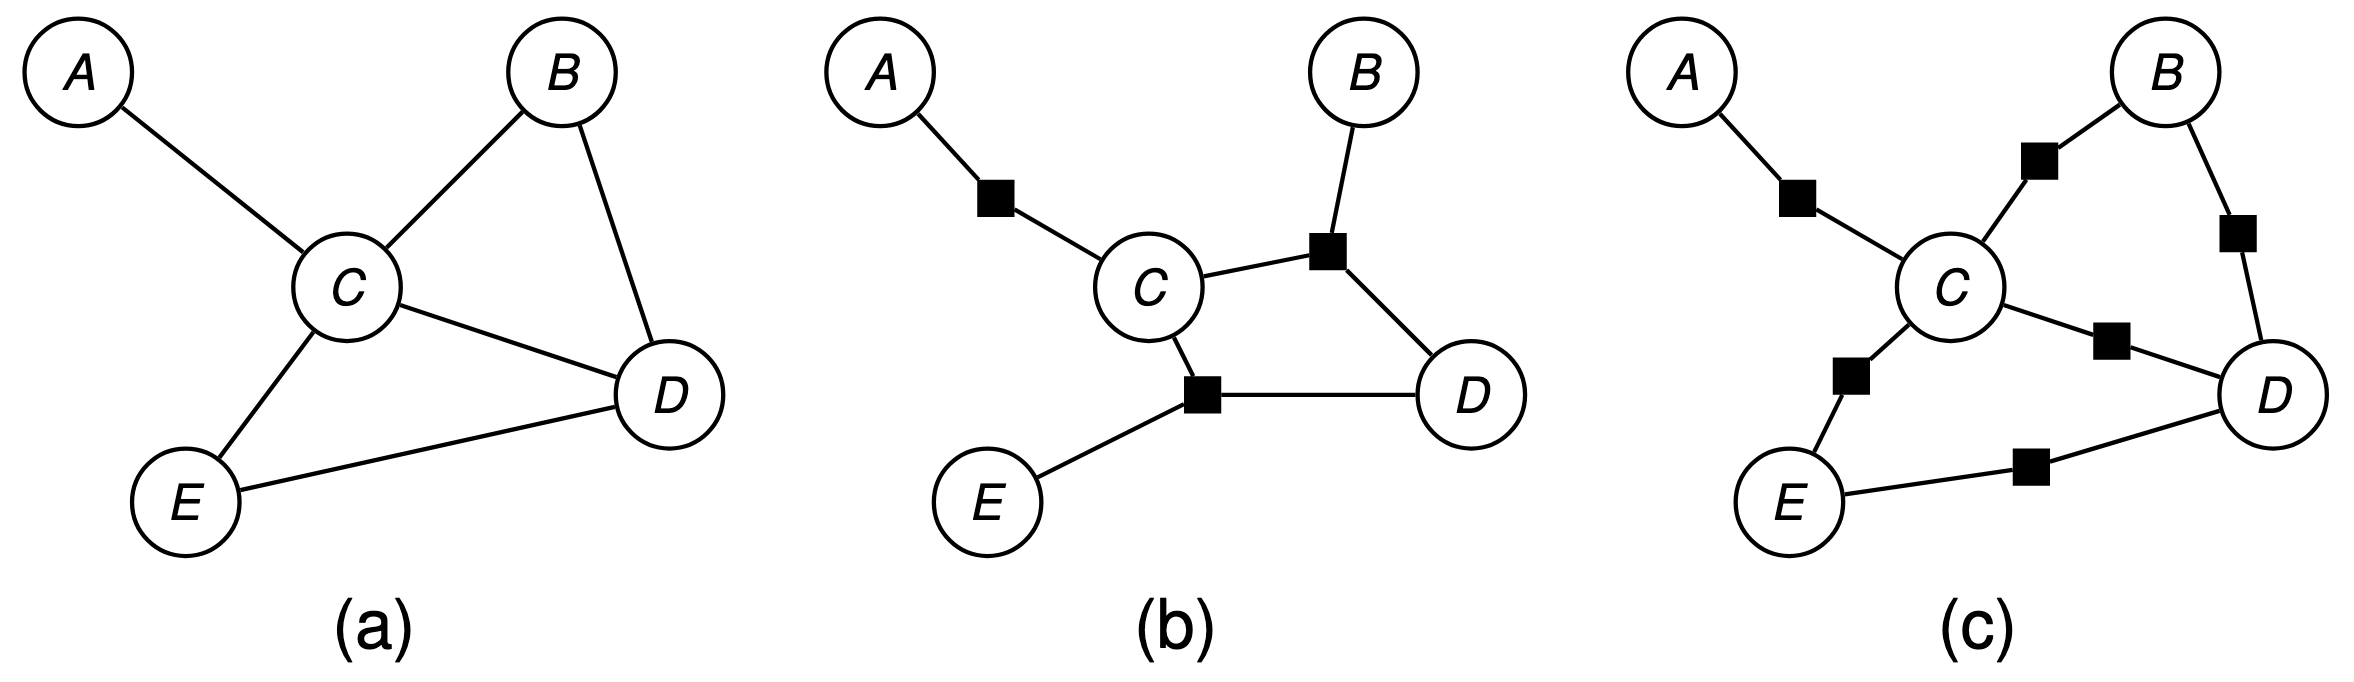
\includegraphics[width=8cm]{img/img1.png}
    \end{figure}  
    Each graph represents exactly the same conditional independent relationship. However, the maximal factorization differs, suppose we have for each variable $K$ possible values:
    \begin{itemize}
        \item $(a)$ can't distiguish between these (we will adopt the $(b)$ to be safe)
        \item $(b)$ has $2$ three-way factor. This is represented in $\mathcal{O}(K^3)$-size table. 
        \item $(c)$ has only pairwise factors. This is represented in $\mathcal{O}(K^2)$-size table. 
    \end{itemize}
    This means that the factor graphs have richer expressive power than undirected graphical models. But the factors can't be determined by testing for conditional independent.
\end{remark}

\begin{remark}{\textbf{(Limitation of Undirected Graphical Model)}}
    Undirected and Factor graph fails to capture the dependencies as the pair of variables that may be connected because they are some other variable that depends on them, for example:
    \begin{figure}[H]
        \centering
        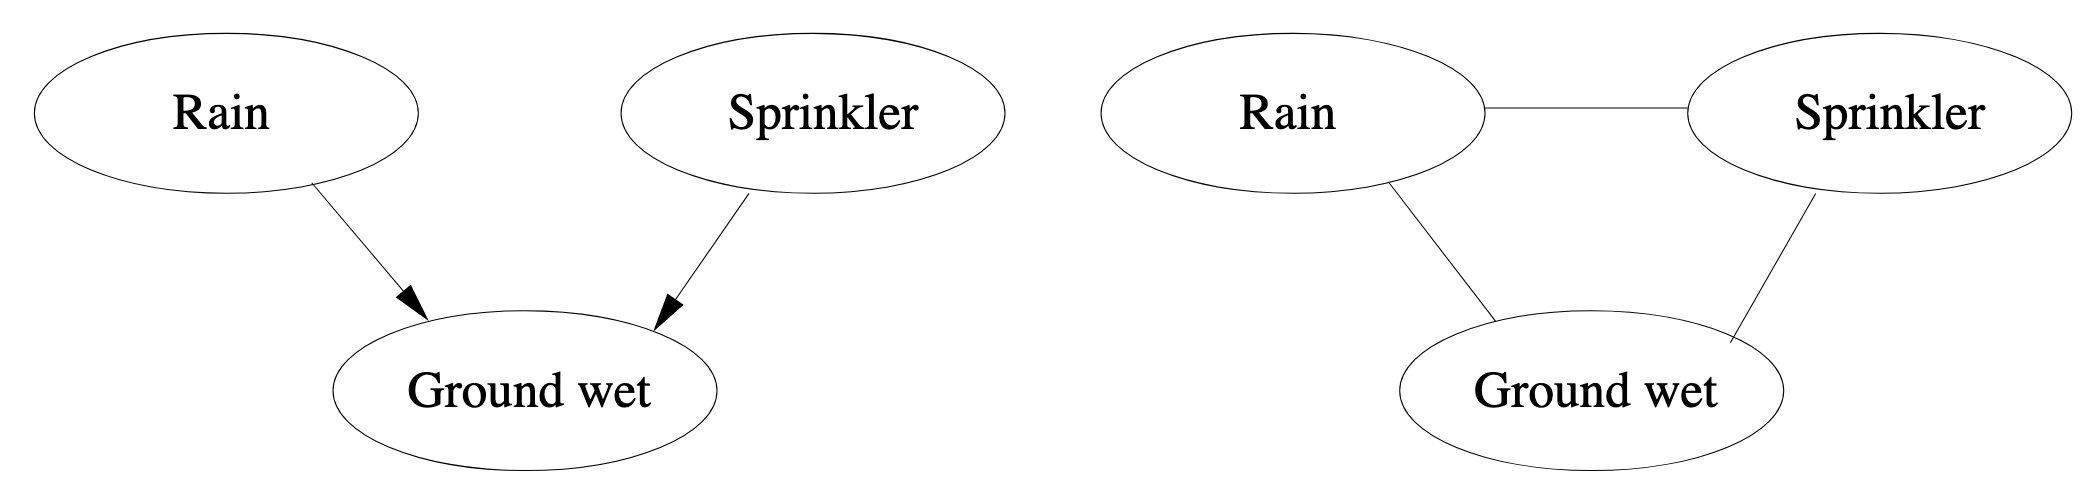
\includegraphics[width=8cm]{img/img2.png}
    \end{figure}  
    If the ground is damped, it may suggest that it was rain, but if we see a sprinkler, then this explain away the damp, thus reduce the our belief of the rain into the prior. For example:
    \begin{equation*}
        R \ind S | \emptyset \quad \text{ but } \quad R\ind S | G
    \end{equation*}
    This is where there is difference between marginal and conditional independent. 
\end{remark}

\begin{definition}{\textbf{(DAG Graphical Model)}}
    A directed acyclic graphical model (DAG) represents a factorization of the joint probability distribution in terms of condtional:
    \begin{equation*}
        P(X_1,\dots,X_n) = \prod^n_{i=1}P(X_i | X_{\text{pa}(i)})
    \end{equation*} 
    where $\text{pa}(\cdot)$ is the parent of node $i$. DAG models are called Baysian network.
\end{definition}

\begin{proposition}
    The conditional Independence between the graph is more complicated than the undirected graph i.e $X\ind Y | \mathcal{V}$. If we consider every undirected path between $X$ and $Y$, the path is blocked by $\mathcal{V}$ if there is a node $V$ on the path such that:
    \begin{itemize}
        \item $V$ has convergnece arrows $\rightarrow V \leftarrow$ on the path and neighbour $V$ nor its descendent are in $\mathcal{V}$
        \item $V$ doesn't have convergnece arrow $\leftarrow V\rightarrow$ or $\rightarrow V \rightarrow$ and $V \in \mathcal{V}$ 
    \end{itemize}
    If all paths are blocked, then $\mathcal{V}$ is $D$-separated between $X$ and $Y$, and so $X\ind Y | \mathcal{V}$. Furthermore, the markov boundary to be:
    \begin{equation*}
        \brackc{\operatorname{pa}(X)\cup\operatorname{ch}(X)\cup\operatorname{pa}(\operatorname{ch}(X))}
    \end{equation*}
\end{proposition}
\begin{proof}
    We can see that the conditional independence of the directed graphical model (for example $A\ind B | \mathcal{D}$) can be modeled as the passing of \correctquote{ball}, in which $2$ variables ($A$, $B$) aren't independence if there is a way that a ball can be passed between them. We will mark the nodes in $\mathcal{V}$ as shaded. There are $10$ simple rules:
    \begin{figure}[H]
        \centering
        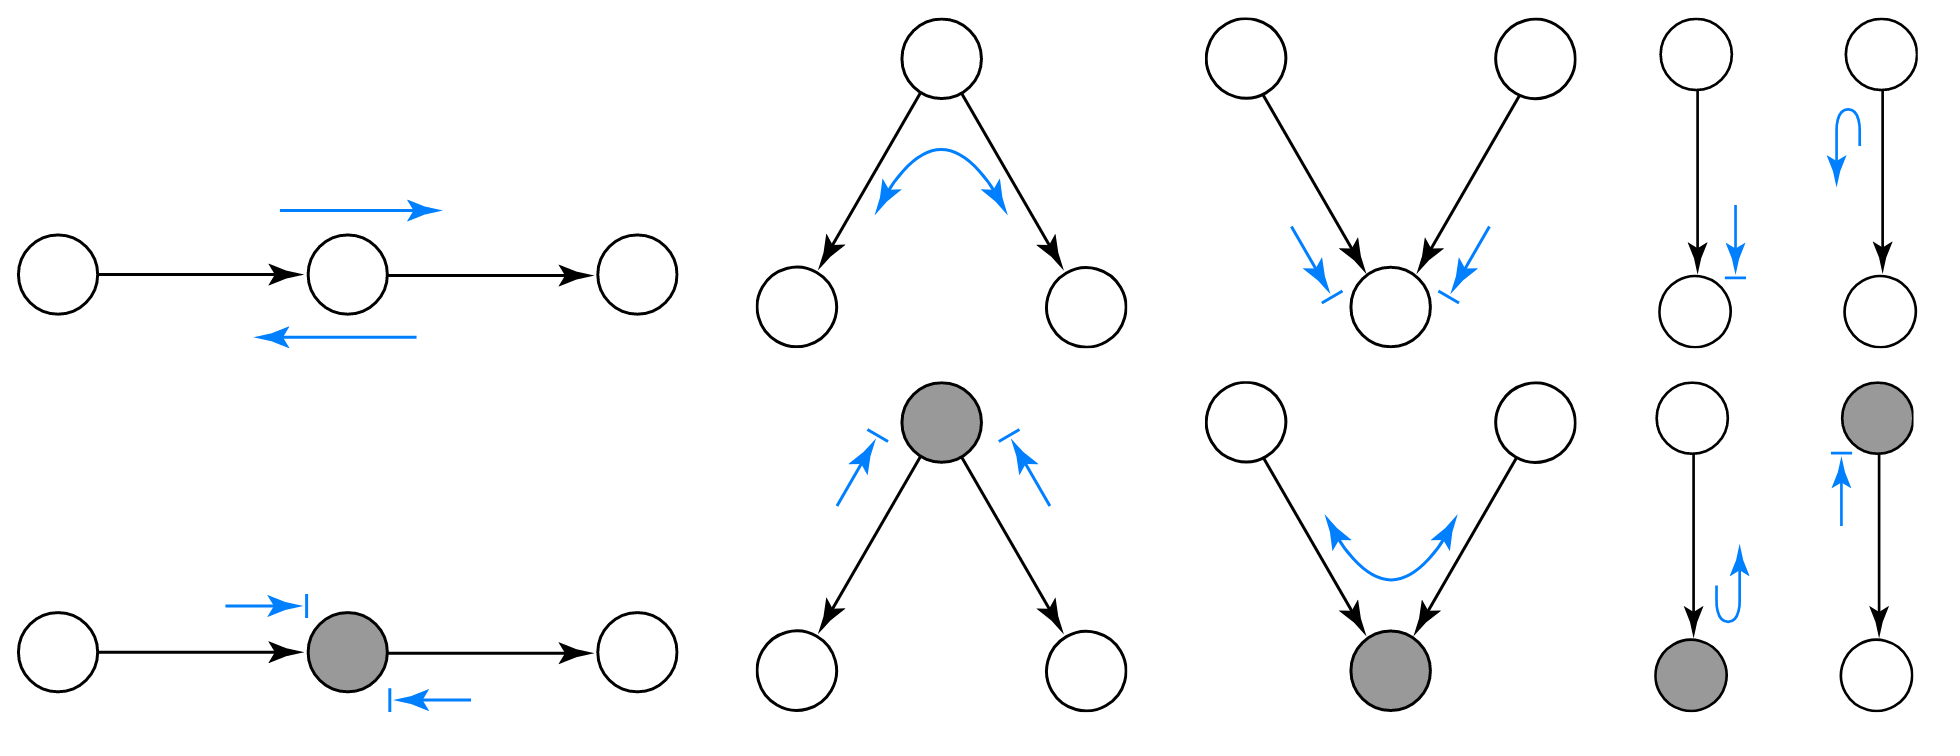
\includegraphics[width=10cm]{img/img3.png}
    \end{figure}  
    Most of the rules are straightforward to see why it is enforced. 
    \begin{itemize}
        \item The first column: Both variables are separated by a middle node, then both of the are independent of each other, thus unable to pass the \correctquote{ball} to each other, meaning that they are independence given the middle node. (This represents the divergence arrow rule)
        \item Similar explaination can be done in the second column of the image. (This also represents the divergence arrow rule)
        \item For the third column (explaining away), we can see that both of the nodes are independence given nothing, however, they becomes dependence once the middle node is shown. This is a reflection of the convergnece arrow rule. 
        \item Finally, the last 2 columns are boundary rule, which is also straightforward to see why it is enforced.
    \end{itemize}
    Thus, we have the reason why the rules above are used. 
\end{proof}

\begin{remark}{\textbf{(Differences Between DAG and Factor Graph)}}
    There are some types of graphs that DAG can represent its probability distribution, which is:
    \begin{figure}[H]
        \centering
        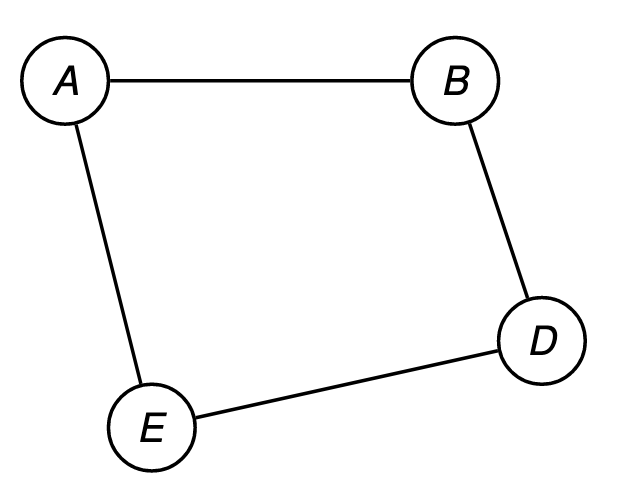
\includegraphics[width=3cm]{img/img4.png}
    \end{figure}  
    This is the only graph that that DAG can't represent. This is because there will always be 2 non-adjecent parent sharing the same child, which implies that:
    \begin{itemize}
        \item The variables are dependence in DAG 
        \item But independence in undirected graph.
    \end{itemize}
    On the other hand, no undirected or factor graph can represent the following DAG and only these:
    \begin{figure}[H]
        \centering
        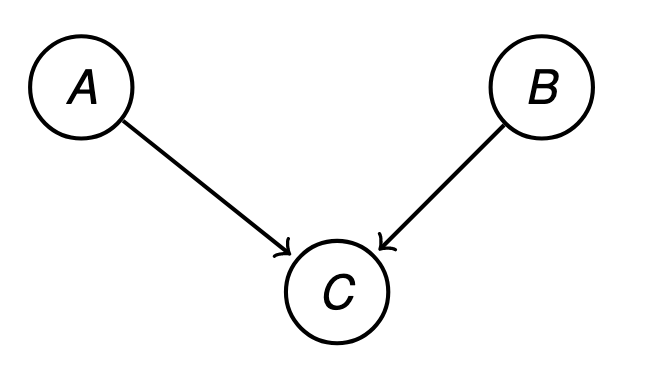
\includegraphics[width=3cm]{img/img5.png}
    \end{figure}  
    This follows from the previous analysis on the explaining away and marginal independence.
\end{remark}

\begin{definition}{\textbf{(Family of Distribution)}}
    Each graph $\mathcal{G}$ implies a set of conditional independence statement: $\mathcal{C}(G) = \brackc{X_i\ind Y_i | \mathcal{Y}}$. Each set $\mathcal{C}$ defines a family of distribution that satisfies all statement in $\mathcal{C}$:
    \begin{equation*}
        P_{\mathcal{C}(G)} = \brackc{P(\mathcal{X}) : P(X_i, Y_i | \mathcal{V}) = P(X_i | \mathcal{V}_i)P(Y_i|\mathcal{Y}_i) \text{ for all } X_i\ind Y_i | \mathcal{V}_i \text{ in } \mathcal{C}  }
    \end{equation*}
    Similarly, we have family distribution in the functional form i.e:
    \begin{equation*}
        P_{G} = \brackc{P(\mathcal{X}) : \frac{1}{Z}\prod_j f_j(\mathcal{X}_{C_j}) \text{ for some non-negative function } f_j }
    \end{equation*}
\end{definition}

\begin{remark}{\textbf{(Family of Distributions)}}
    We can consider the following facts:
    \begin{itemize}
        \item For directed graph: $P_G = P_{\mathcal{C}(G)}$
        \item For undirected graph: $P_G = P_{\mathcal{C}(G)}$ if all distribution are positive i.e $P(\mathcal{X})>0$ for all variable of $\mathcal{X}$
        \item Factor graphs are more expressive as for every undirected graph $G_1$, there is a factor graph $G_2$ such that: $P_{G_1} = P_{G_2}$ but not in other direction.
    \end{itemize}
    Adding edge implies removing conditional independency statement and thus enlarging family of distribution.
\end{remark}

\begin{remark}
    For the next few propositions, we will consider difference kinds of graphical models, which can be shown to interchange with each others:
    \begin{figure}[H]
        \centering
        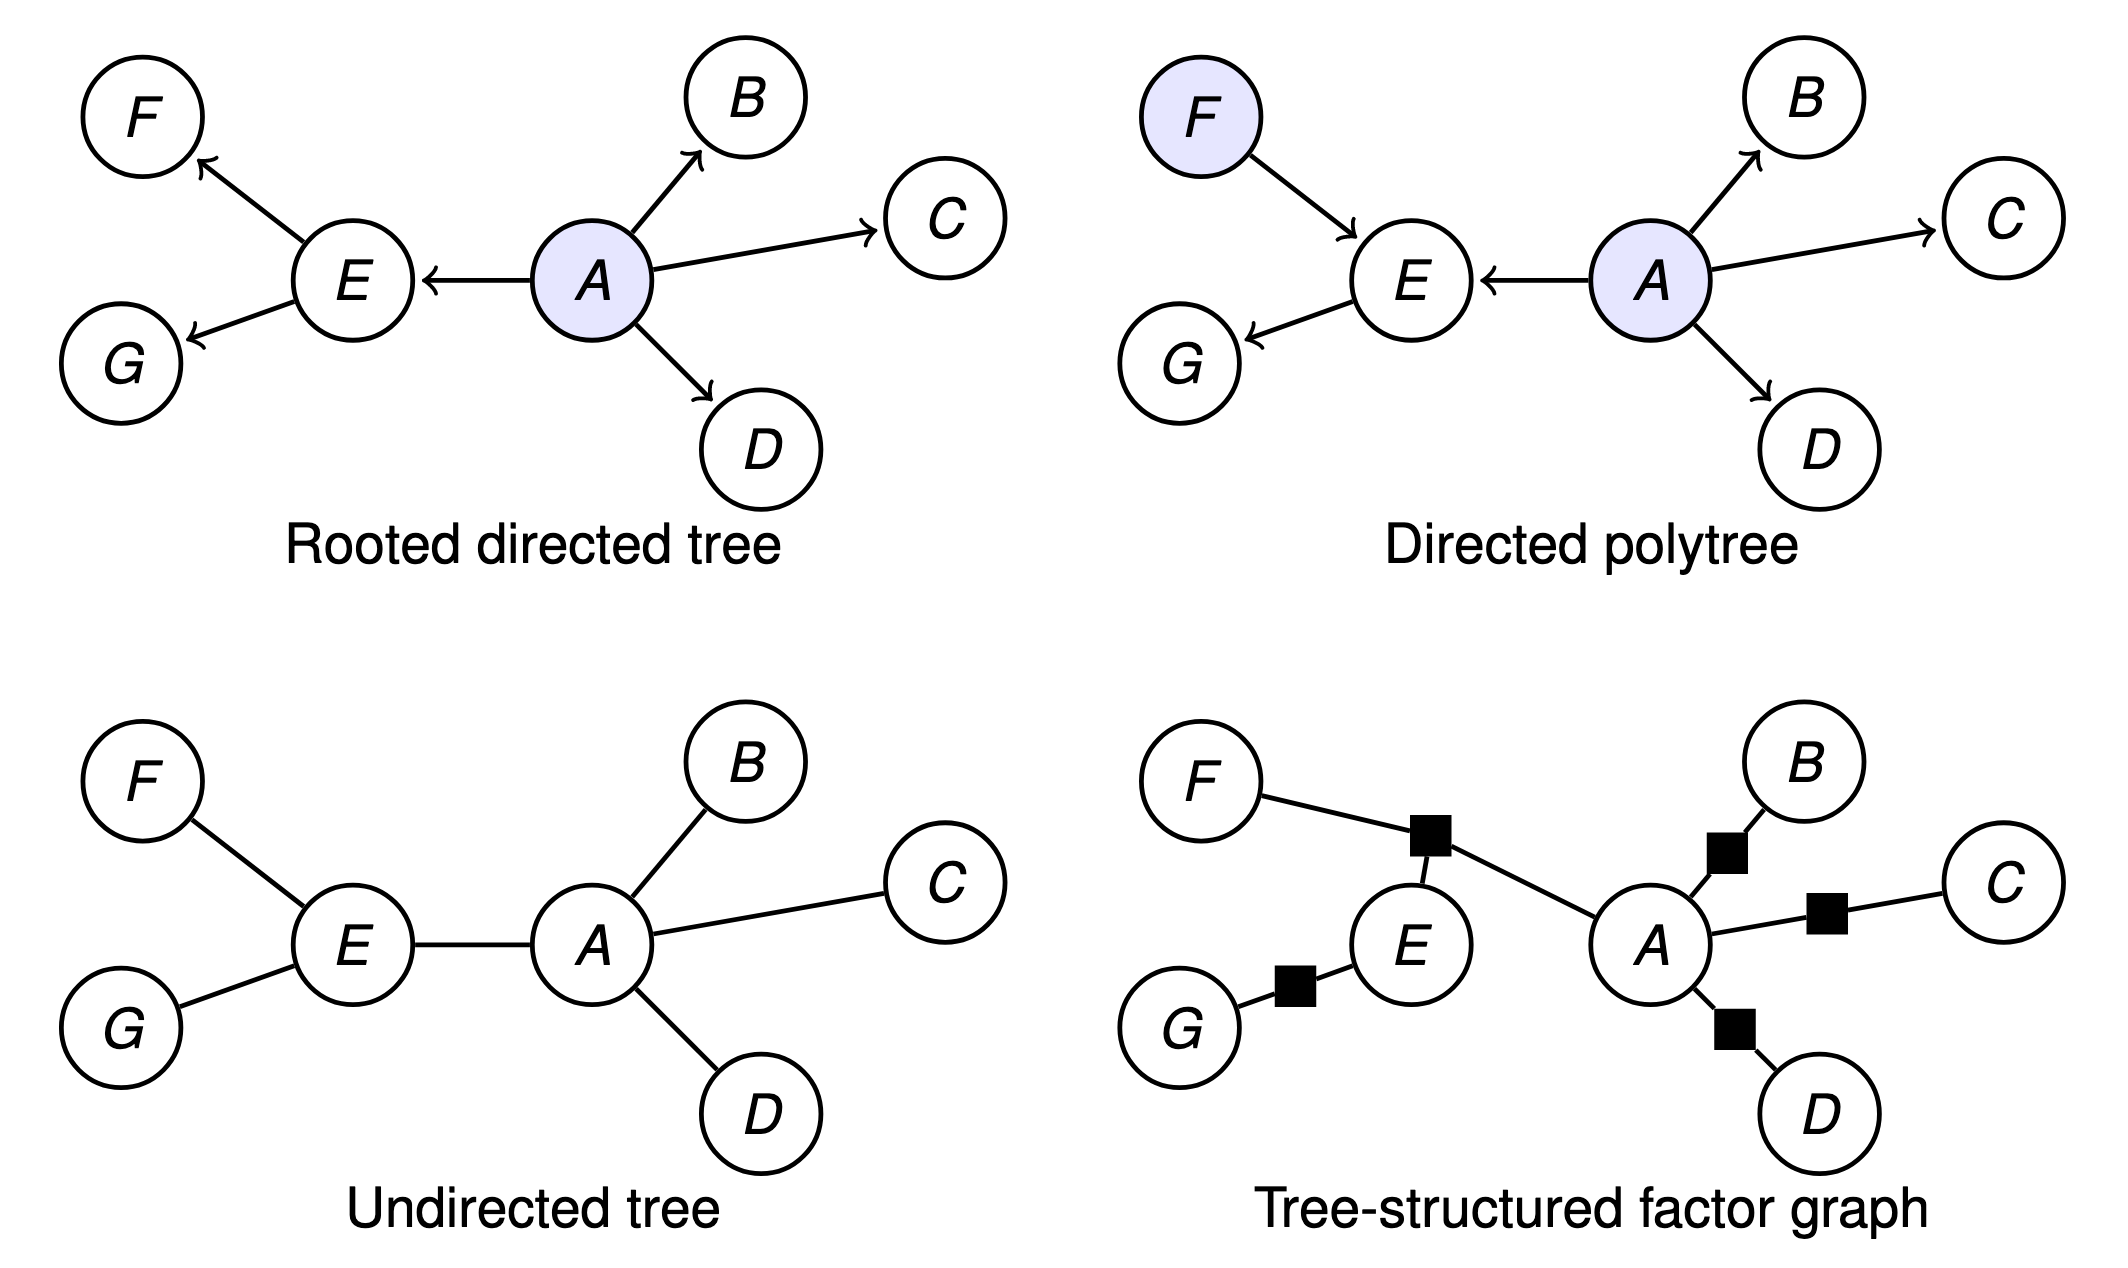
\includegraphics[width=8cm]{img/img6.png}
    \end{figure}  
\end{remark}

\begin{proposition}{\textbf{(Polytree $\boldsymbol \rightarrow$ Tree-Structured Factor Graph)}}
    For DAG that has more than one root, we consider:
    \begin{equation*}
        P(\mathcal{X}) = \prod_i P(X_i | X_{\text{pa}(i)}) =\prod_if_i(X_{C_i})
    \end{equation*} 
    where $C_i = i \cup \operatorname{pa}(i)$ and $f(X_{C_i}) = P(X_i | X_{\operatorname{pa}(i)})$
\end{proposition}

\begin{proposition}{\textbf{(Undirected Tree $\boldsymbol \rightarrow$ Factor Graph)}}
    Since all undirected tree have maximal clique of size $2$, it is equivalent to factor graph with pairwise factor:
    \begin{equation*}
        P(\mathcal{X}) = \frac{1}{Z}\prod_{\operatorname{edge}(i,j)}f_{(i,j)}(X_i, X_j)
    \end{equation*}
\end{proposition}

\begin{proposition}{\textbf{(Rooted Directed Tree $\boldsymbol \rightarrow$ Undirected Tree)}}
    The distribution for single rooted directed tree can be written as a product of pairwise factor of the undirected tree:
    \begin{equation*}
        P(\mathcal{X}) = P(X_r)\prod_{i\ne r}P(X_i | X_{\operatorname{pa}(i)}) = \prod_{\operatorname{edge}(i,j)}f_{(i,j)}(X_i, X_j)
    \end{equation*} 
\end{proposition}

\begin{proposition}{\textbf{(Undirected Tree $\boldsymbol \rightarrow$ Rooted Directed Tree)}}
    Choose arbitary node $X_r$ and set it as a root, which we will point every arrow away from it. Compute the conditional in the DAG as:
    \begin{equation*}
        P(\mathcal{X}) = P(X_r) \prod_{i\ne r}P(X_i|X_{\operatorname{pa}(i)}) = P(X_r)\prod_{i\ne r}\frac{P(X_i, X_{\operatorname{pa}(i)})}{P(X_{\operatorname{pa}(i)})} = \frac{\prod_{\operatorname{edge}(ij)}P(X_i,X_j)}{\prod_{\operatorname{nodes}(i)} P(X_i)^{\operatorname{deg}(i)- 1}}
    \end{equation*}
\end{proposition}

\section{Belief Propagation}

\begin{remark}
    We want to calculate the marginal distribution of a single node $P(X_i)$ and on the edge $P(X_i, X_j)$ based on the undirected graphical model, which we would need to use a belief propagation.
\end{remark}

\begin{proposition}{\textbf{(Marginal Distribution)}}
    The marginal distribution can be calculated locally as:
    \begin{equation*}
        P(X_i) = \prod_{X_j \in \operatorname{ne}(i)} M_{j\rightarrow i} \quad \text{ where } \quad M_{j\rightarrow i} = \sum_{X_j}f_{ij}(X_i, X_j) \prod_{X_k \in \operatorname{ne}(X_j)\backslash\brackc{X_i}} M_{k\rightarrow j}(X_j)
    \end{equation*}
\end{proposition}    
\begin{proof}
    For each neighbourhood $X_j$ of $X_i$ define a disjoint subtree $T_{j\rightarrow i}$ that split by $X_i$:
    \begin{equation*}
    \begin{aligned}
        P(X_i) &= \sum_{\mathcal{X}\backslash\brackc{X_i}} P(\mathcal{X}) \propto \sum_{\mathcal{X}\backslash\brackc{X_i}}\prod_{(i, j)\in \mathcal{E}_T} f_{ij}(X_{i}, X_{j}) \\
        &= \sum_{\mathcal{X}\backslash\brackc{X_i}}\prod_{X_j \in \operatorname{ne}(X_i)}f_{ij}(X_i, X_j)\prod_{(i', j')\in\mathcal{E}_{T_{j\rightarrow i}}}f_{i'j'}(X_{i'}, X_{j'}) \\
        &= \prod_{X_j \in \operatorname{ne}(i)} \bracka{\sum_{\mathcal{X}_{T_{j\rightarrow i}}} f_{ij}(X_i, X_j) \prod_{(i',j')\in\mathcal{E}_{T_{j\rightarrow i}}} f_{i'j'}(X_{i'}, X_{j'}) }
    \end{aligned}
    \end{equation*}
    The last equality comes from the splitting between subtrees, as they are disjoint. $\mathcal{X}_{T_{j\rightarrow i}}$ denotes each edge in the subtree. Let's consider the message:
    \begin{equation*}
    \begin{aligned} 
        M_{j\rightarrow i} 
        &= \sum_{\mathcal{X}_{T_{j\rightarrow i}}} f_{ij}(X_i, X_j) \prod_{(i',j')\in\mathcal{E}_{T_{j\rightarrow i}}} f_{i'j'}(X_{i'}, X_{j'})  \\ 
        &= \sum_{X_j} f_{ij}(X_i, X_j)\sum_{\mathcal{X}_{T_{j\rightarrow i}}\backslash \brackc{X_j}} \prod_{(i',j')\in\mathcal{E}_{T_{j\rightarrow i}}} f_{i'j'}(X_{i'}, X_{j'}) \\
        &= \sum_{X_j} f_{ij}(X_i, X_j) \prod_{X_{k}\in\operatorname{ne}(X_j)\backslash X_i} M_{k\rightarrow i}(X_j)
    \end{aligned}
    \end{equation*}
    The second equality comes from the fact that the factor of $X_i$ is the root of the tree and for any nodes that connection to the factors. If we consider:
    \begin{equation*}
    \begin{aligned}
        \sum_{\mathcal{X}_{T_{j\rightarrow i}}\backslash \brackc{X_j}} \prod_{(i',j')\in\mathcal{E}_{T_{j\rightarrow i}}} f_{i'j'}(X_{i'}, X_{j'}) &\propto P_{T_{j\rightarrow i}}(X_j) \\
        &\propto \prod_{X_{k}\in\operatorname{ne}(X_j)\backslash X_i} M_{k\rightarrow i}(X_j)
    \end{aligned}
    \end{equation*}
    This is due to recursive property of the message passing.
\end{proof}

\begin{proposition}{\textbf{(Pairwise Marginal)}}
    \begin{equation*}
        P(X_i, X_j) = f_{ij}(X_i,X_j)\prod_{X_k \in \operatorname{ne}
        (X_j)\backslash \brackc{X_i} }M_{k\rightarrow j}(X_j) \prod_{X_k\in\operatorname{ne}(X_i)\backslash\brackc{X_j}} M_{k\rightarrow i}(X_i)
    \end{equation*}
\end{proposition}
\begin{proof}
    We consider:
    \begin{equation*}
    \begin{aligned}
        P(X_i, X_j) &= \sum_{X\backslash\brackc{X_i, X_j}}P(\mathcal{X}) \propto \sum_{X\backslash\brackc{X_i, X_j}}\prod_{(i,j)\in\mathcal{E}_T}f_{ij}(X_i, X_j) \\
        &= \sum_{X\backslash\brackc{X_i, X_j}}f_{ij}(X_i, X_j)\prod_{(i'j')\in\mathcal{E}_{T_{j\rightarrow i}}}f_{i'j'}(X_{i'}, X_{j'})\prod_{(i'j')\in\mathcal{E}_{T_{i\rightarrow j}}}f_{i'j'}(X_{i'}, X_{j'}) \\
        &= f_{ij}(X_i, X_j)\bracka{\sum_{\mathcal{X}_{T_{j\rightarrow i}}} \prod_{(i'j')\in\mathcal{E}_{j\rightarrow i}} f_{i'j'}(X_{i'}, Y_{j'}) }\bracka{ \sum_{\mathcal{X}_{T_{i\rightarrow j}}}\prod_{(i'j')\in\mathcal{E}_{T_{i\rightarrow j}}} f_{i'j'}(X_{i'}, Y_{j'}) } \\
        &= f_{ij}(X_i,X_j)\prod_{X_k \in \operatorname{ne}
        (X_j)\backslash \brackc{X_i} }M_{k\rightarrow j}(X_j) \prod_{X_k\in\operatorname{ne}(X_i)\backslash\brackc{X_j}} M_{k\rightarrow i}(X_i)
    \end{aligned}
    \end{equation*}
\end{proof}

\begin{remark}{\textbf{(Belief Propagation for Inference)}}
    Let's consider the belief propagation for inference on the following graphical model:
    \begin{figure}[H]
        \centering
        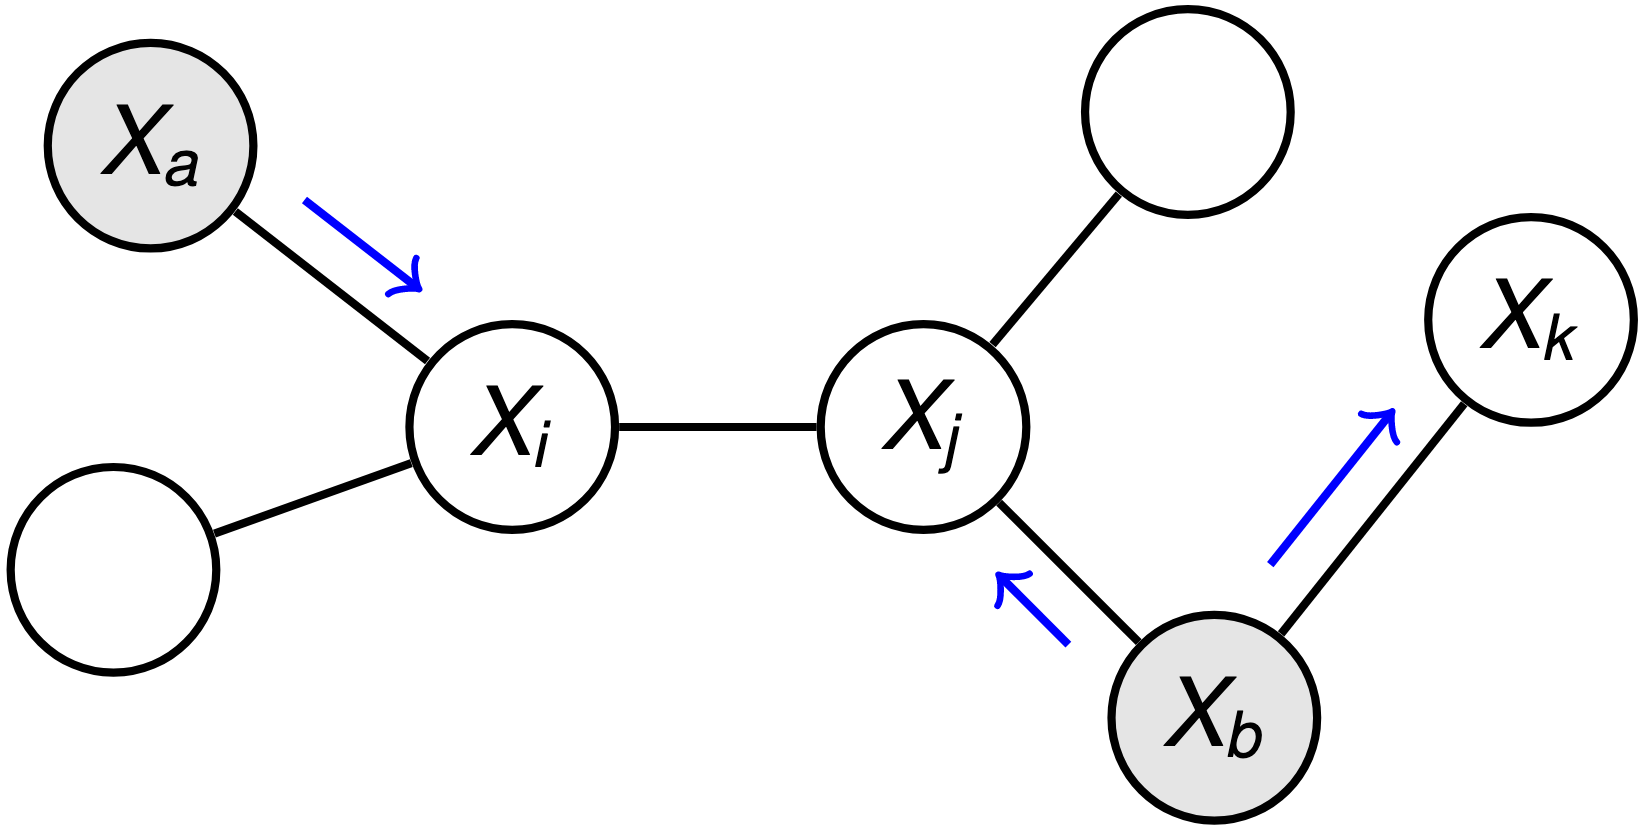
\includegraphics[width=8cm]{img/img7.png}
    \end{figure}  
    To compute the $P(X_i | X_a = a)$ as we have the following message:
    \begin{equation*}
        M_{a\rightarrow i} = f_{ai}(X_a = a, X_i)
    \end{equation*}
    Please note that computing $P(X_i)$ requires that $M_{a\rightarrow i} = \sum_{X_a}f_{ai}(X_a, X_i)$. 
    For the internal node that partition the graph, like variable like $X_b$, we have the following message:
    \begin{equation*}
        M_{b\rightarrow j} = f_{bj}(X_b = b, X_j) \qquad M_{b\rightarrow k} = f_{bk}(X_b = b, X_k)
    \end{equation*}
    Please note that $M_{i\rightarrow j}$ are proportional to likelihood based on any observed variable (within message subtree) and possibly scaled by the prior (depends on factorization):
    \begin{equation*}
        M_{i\rightarrow j}(X_j) \propto P(\mathcal{X}_{T_{i\rightarrow j}}\cap\mathcal{O} | X_j)P(X_j)
    \end{equation*}
    If we consider the message to the observed node, then we have the likelihood. Keeepin all messages unnormalize and any marginal, then the normalizer is the likelihood. 
\end{remark}

\begin{remark}{\textbf{(BP Latent Chain Model)}}
    We consider the belief propagation in the latent chain model, which is a rooted directed tree, as we have the following graphical model:
    \begin{figure}[H]
        \centering
        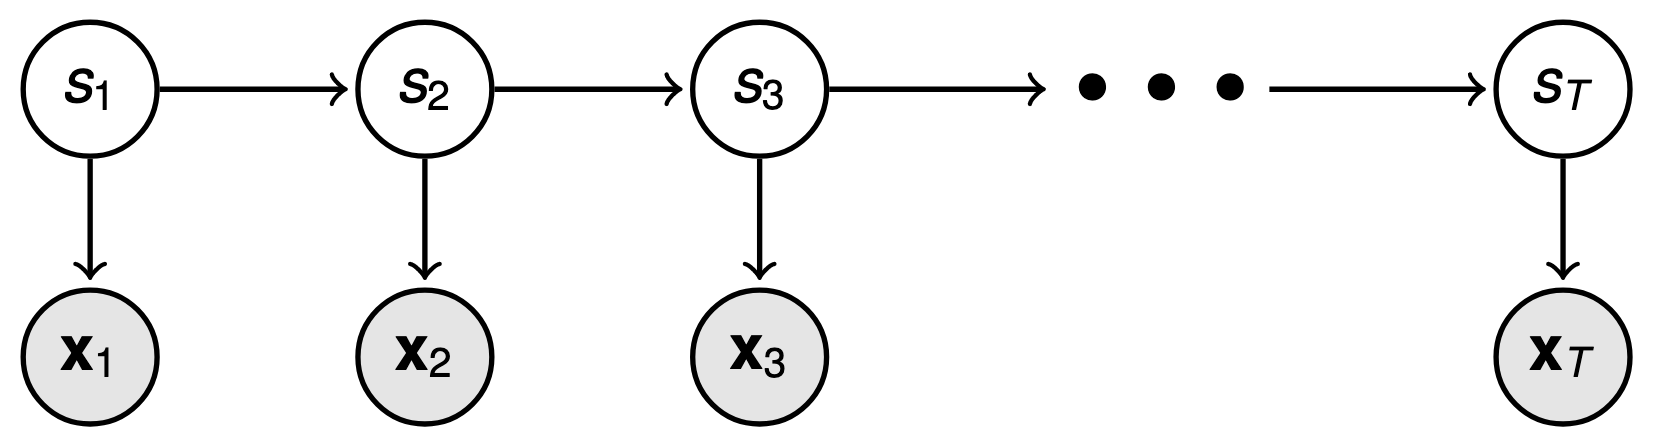
\includegraphics[width=8cm]{img/img8.png}
    \end{figure}  
    We use the backward-forward algorithm is just belief propagation on this graph:
    \begin{itemize}
        \item $\alpha_t(i) = M_{s_{t-1}\rightarrow s_t}(s_t = i) \propto P(x_{1:t}, s_t)$ 
        \item $\beta_t(i) = M_{s_{t+1}\rightarrow s_t}(s_t = i)\propto P(x_{t+1: T} | s_t)$
    \end{itemize}
    where we can easily see that:
    \begin{equation*}
        \alpha_t(i)\beta_t(i) = \prod_{j\in\operatorname{ne}(s_t)} M_{j\rightarrow s_t}(s_t = i) \propto P(s_t = i | \mathcal{O}) 
    \end{equation*}
    The algorithm like BP extend the power of graphical model beyound just encoding of independent and factorization. A single derivation surves multiple models.
\end{remark}

\subsection{Junction Tree}

\begin{remark}{\textbf{(Inference on Graph)}}
    The graphical model sometimes, which is represented by an undirected graph isn't a tree as we would like to find the marginal probability of the single value. There are several strategies that we can use:
    \begin{itemize}
        \item Propagate the local message anyway and hope for the best. This is called \correctquote{loopy belief propagation}, which is an approximation technique. 
        \item Grouping the variable together with multi-variable nodes until the resulting graph, which is a tree as we are going consider this. 
    \end{itemize}
\end{remark}

\begin{remark}{\textbf{(Transforming the Graph)}}
    Consider to transform the graph into one that is easier to handle. As the original graph $G$ encodes a distribution $P(\mathcal{X})$ with a certain factorization or independent structure:
    \begin{itemize}
        \item Transformation from $G$ into an easy to handle $G'$ as it will be valid if $P(\mathcal{X})$ can be represented by $G'$
        \item Ensuring this, we need every step of the graph transformation only to remove condtional independence (never adding them).
        \item Making the family of possible encoding distribution groups grows or stay the same at each step. 
        \item The factor potential on the new graph $G'$ are built from those given on $G$ as to make sure it encodes the same distribution.  
    \end{itemize}    
\end{remark}

\begin{definition}{\textbf{(Junction Tree)}}
    A junction tree is a tree whose node and edges are labelled with set of variables. 
    \begin{itemize}
        \item Each node is represented by a cliques, edges are labelled by intersection of cliques called seperator. 
        \item The cliques contains all adjacent separator. 
        \item Furthermore, if $2$ cliques contain variable $X$, all cliques and separator on the path between $2$ cliques must contain $X$
    \end{itemize}
\end{definition}

\begin{definition}{\textbf{(Constructing Junction Tree)}}
    We consider the following step that transform DAG into a junction tree, which is shown in the figure below:
    \begin{figure}[H]
        \centering
        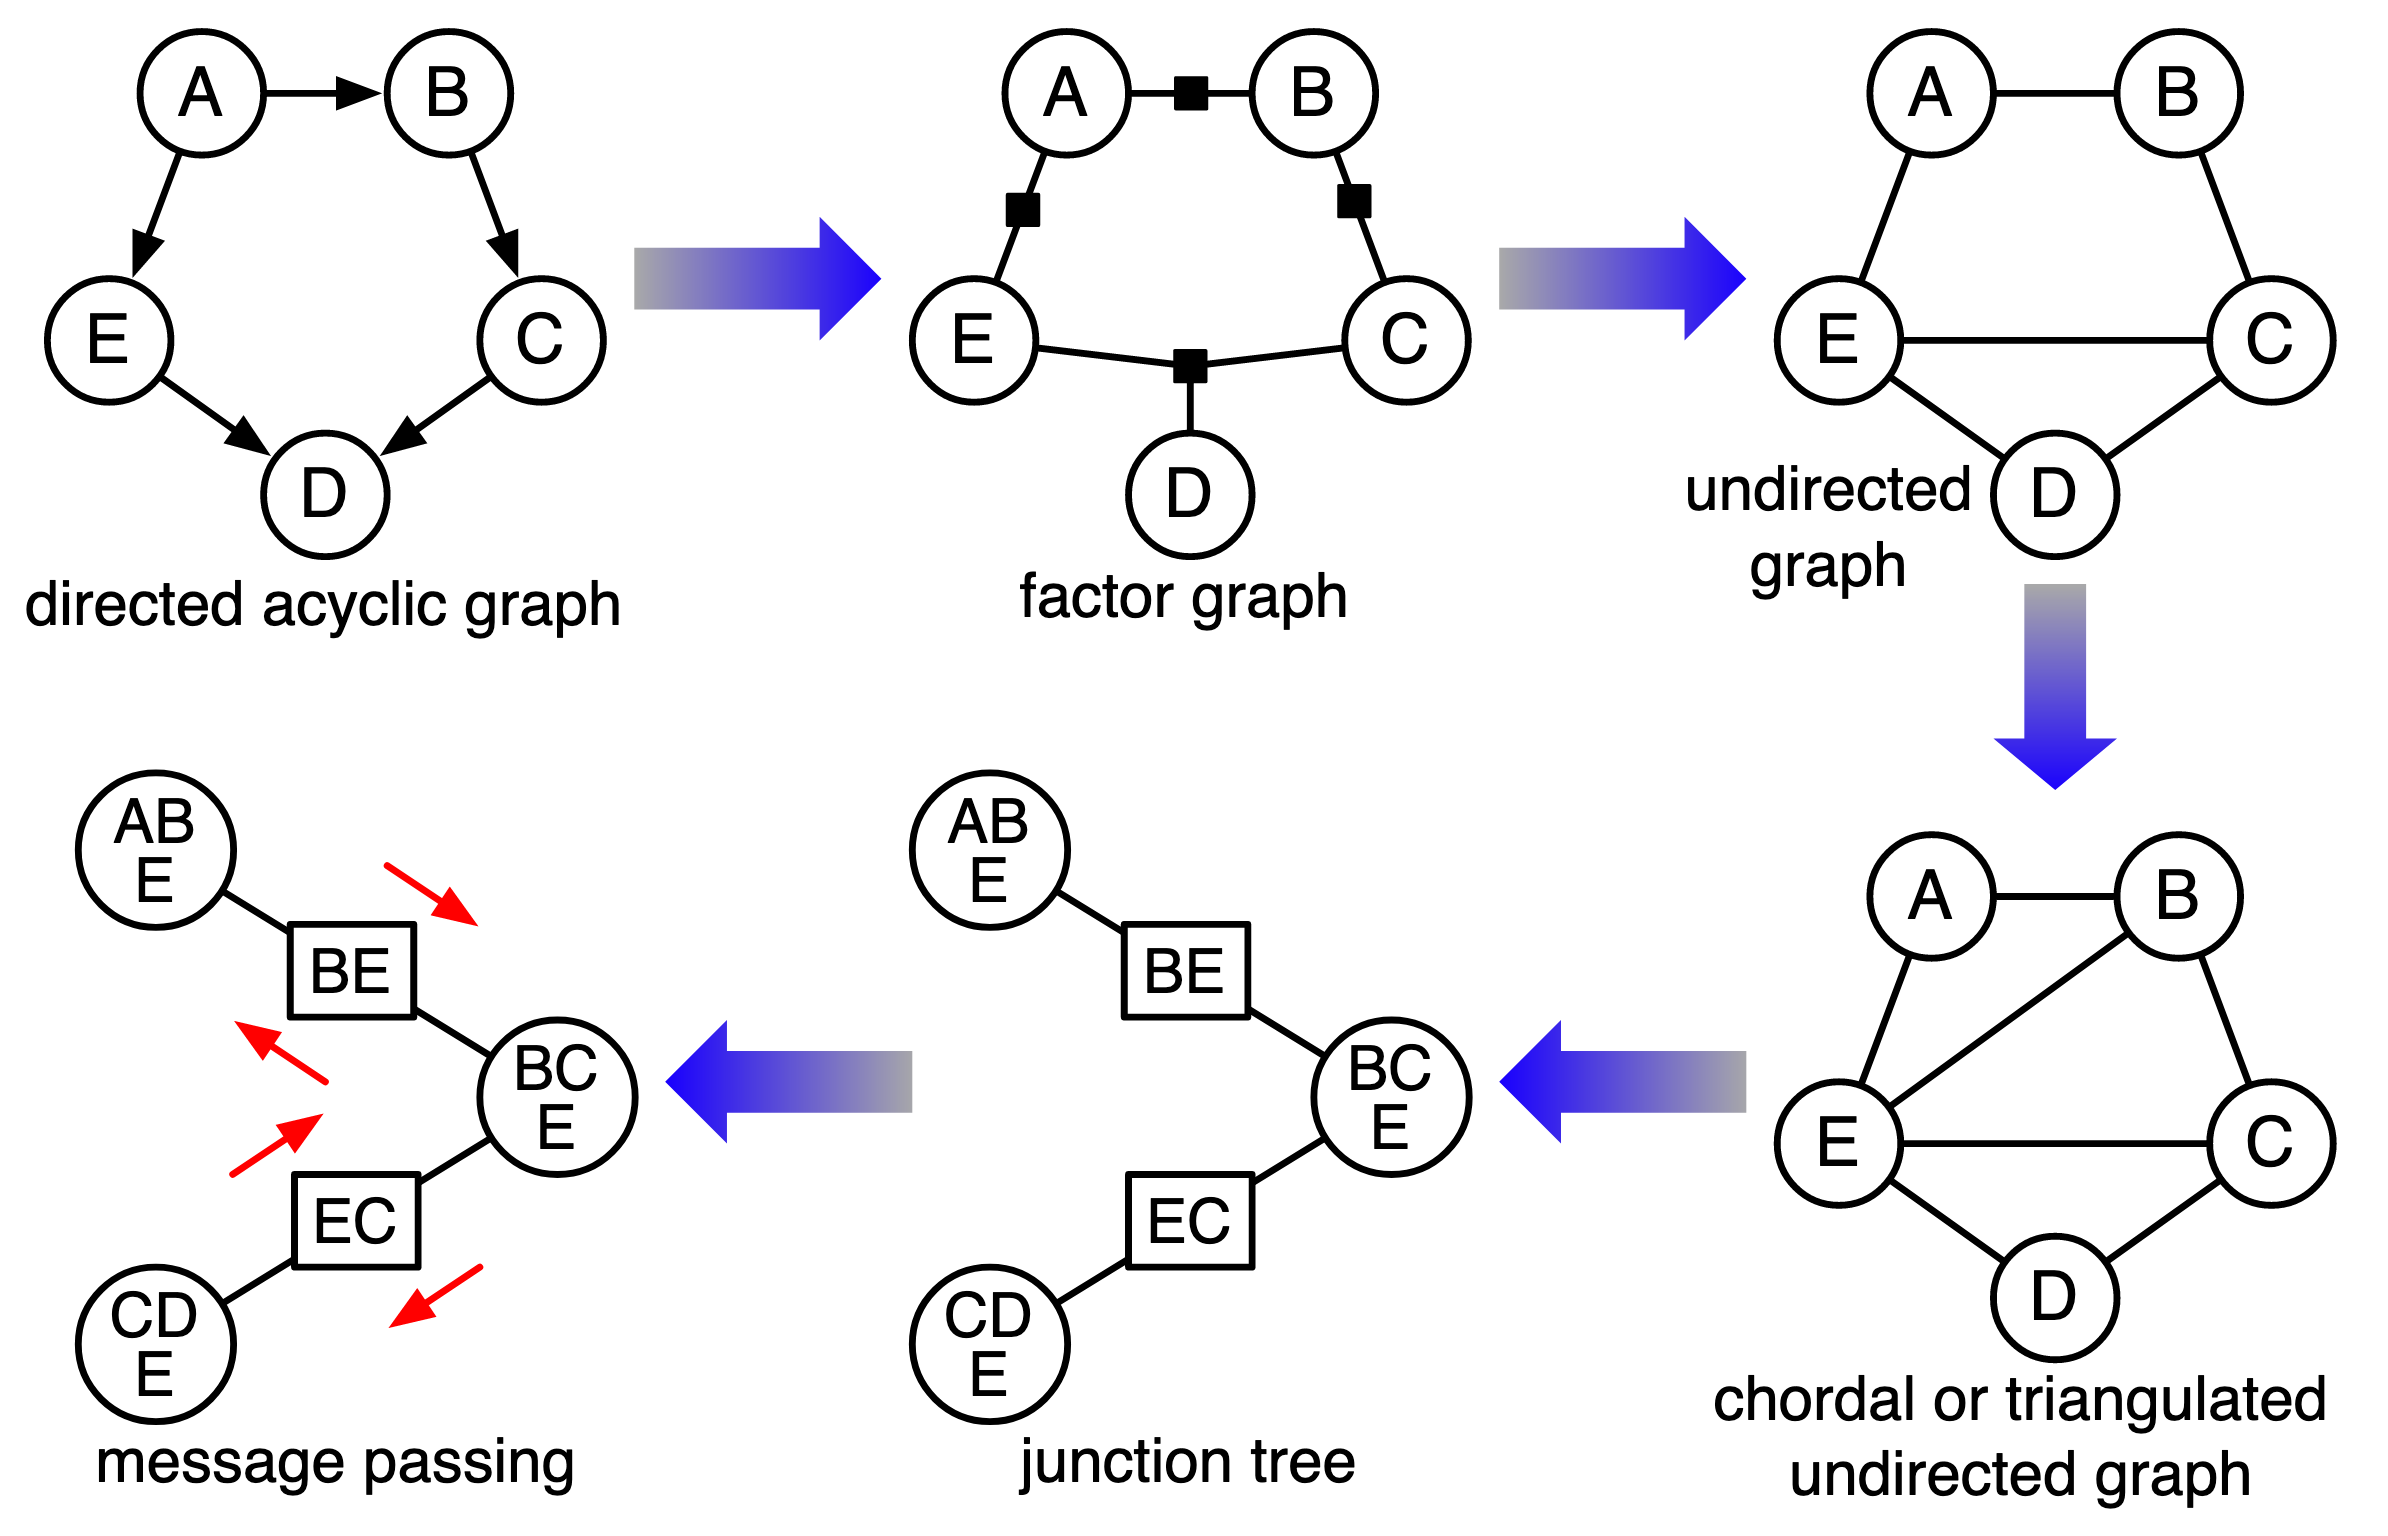
\includegraphics[width=8cm]{img/img9.png}
    \end{figure}  
    There are many process that we have to perform. 

    \textbf{DAG to Factor Graph:} The factor can be see as the conditional distribution of DAG via:
    \begin{equation*}
        P(\mathcal{X}) = \prod_iP(X_i|X_{\operatorname{pa}(i)}) = \prod_if_i(X_C)
    \end{equation*}
    where $C_i = i\cup \operatorname{pa}(i)$ and $f_i(X_{C_i}) = P(X_i|X_{\operatorname{pa}(i)})$. Marginal distribution on roots $P(X_r)$ absorbed into an adjacent factor.

    \textbf{Observation in Factor Graph:} Usually, inference target a posterior marginal given a set of observed values $P(X_l|\mathcal{O})$; for example, $P(A | D =\text{wet}, C = \text{rain})$. Modify the factor linked to the observed node, or add single factor adjacent to the observed node:
    \begin{equation*}
        f_D(D) = \begin{cases}
            1 &\text{ if } D = \text{wet} \\
            0 &\text{ otherwise }
        \end{cases} \qquad f_C(C) = \begin{cases}
            1 &\text{ if } C = \text{rain} \\
            0 &\text{ otherwise }
        \end{cases}
    \end{equation*}
    
    \textbf{Factor Graph to Undirected Graph:} The trasnformation from DAG to undirected graph is called moralization, where: Marry all parents of each node by adding an edge to connect them. We also drop arrows on all edges. 

    \textbf{Triangulate the Undirected Graph:} Want every factor of DAG must be contained within a maximal cliques of the undirected graph. We will have to perform the following modification:
    \begin{itemize}
        \item Replace each factor by an undirected cliques. 
        \item Construct the potential on each maximal clique by multiplying together factor potential that fall on it, and ensure each factor potential only appear once. 
    \end{itemize}
    To do this, we shall modify the graph as:
    \begin{itemize}
        \item We join the loop into cliques, which can be very inefficient. 
        \item Triangulation is performed to add edges to graph, so that every loop of size $\ge4$ has at least one chord. We will adding it recursively to ensure that the loop $\ge4$ has chords too. 
        \item The graph where every loop of size $\ge4$ has at least one chord is called chordal or triangulated. 
        \item Adding the edge removes conditional independencies, which enlarge the family of distribution. 
    \end{itemize}
    To find the triangulation is NP-complete problem, so we resort to heuristic called variable elimination. Let's consider the order of elimination as we have:
    \begin{equation*}
    \begin{aligned}
        P(X_{(n)}) &= \sum_{X_{\sigma(n-1)}}\cdots\sum_{X_{\sigma(1)}} P(\mathcal{X}) \\
        &= \frac{1}{Z}\sum_{X_{\sigma(n-1)}}\cdots\sum_{X_{\sigma(1)}} \prod_i f_i(\mathcal{X}_{C_i}) \\
        &= \frac{1}{Z}\sum_{X_{\sigma(n-1)}}\cdots\sum_{X_{\sigma(2)}}\prod_{j : C_j \ni \sigma(2)}f_j(\mathcal{X}_{C_j})\sum_{X_{\sigma(1)}} \prod_{i:C_i\ni\sigma(1)}f_i(\mathcal{X}_{C_i}) \\
        &= \frac{1}{Z}\sum_{X_{\sigma(n-1)}}\cdots\sum_{X_{\sigma(2)}}\prod_{j : C_j \ni \sigma(2)}f_j(\mathcal{X}_{C_j})f_\text{new}(\mathcal{X}_\text{new})
    \end{aligned}
    \end{equation*}
    Please note that $C_\text{new}$ is the neighbour of $X_{\sigma(1)}$ and \emph{edges are added to graph connected all nodes in} $C_\text{new}$:
    \begin{itemize}
        \item The graph including of all edges would be induced by elimination is chordal. 
        \item Finding a good triangulation depends on findinga good order of elimination $\sigma(1),\dots,\sigma(n)$. 
        \item It is NP-complete to find the best heuristic, as there are $2$ ways that we pick the next varaible to elimiate as follows:
        \begin{itemize}
            \item Min-Deficiency Search: Choose variable that induces the fewest new edge. 
            \item Max-Cardinal Search: Choose node with most previous visited neighbour.
        \end{itemize}
        In most experiments, min-deficiency search seem empirically be better. 
    \end{itemize}
    \textbf{Chordal Graph to Junction Tree:} To build a junction tree, we follows the procedure as we have:
    \begin{itemize}
        \item Find the maximal clique $C_1,\dots,C_k$ of the chordal undirected graph. 
        \item Create a weighted graph, which nodes are labelled by maximal cliques and edges connected each pair of cliques that shares variables. 
        \item Create an edge with size of separator as we find maximal weight spanning tree of weighted graph. 
    \end{itemize}
    Thus, we have the junction tree.
\end{definition}

\begin{remark}{\textbf{(Junction Tree Figures)}}
    The joint distribution factors over junction tree is:
    \begin{equation*}
        P(\mathcal{X})  = \frac{1}{Z}\prod_if_i(X_{C_i}) = \dots f_\text{ABC}(A, B, C)f_\text{BCD}(B, C, D)\dots
    \end{equation*}
    This violates the usual undirected tree sematics of factor per edge, and so we add the following constriants:
    \begin{itemize}
        \item Introducing the copy of the same variable so that there is no overlaps. 
        \item Adding new delta function that enforce consistency:
        \begin{equation*}
            P(\mathcal{X}) = \dots f_\text{ABC}(A, B^{(1)}, C^{(1)})\underbrace{\delta(B^{(1)} - B^{(2)})\delta(C^{(1)}, C^{(2)})}_{f_\text{sep}(B^{(1)}, C^{(1)}, B^{(2)}, C^{(2)})}f_\text{BCD}(B^{(2)}, C^{(2)}, D)\dots
        \end{equation*}
    \end{itemize}
    Having a new message passing the junction to be:
    \begin{itemize}
        \item Unshared Variable $X^{(-)}_{C_i} = X_{C_i \backslash \bigcup S_{ik}}$
        \item Variable incoming separator $X^{(2)}_{S_{ki}}$ (Same as matching variable $X^{(1)}_{S_{ki}}$ in $k\in\operatorname{ne}(i)\backslash j$)
        \item Variable outgoing separator $X^{(1)}_{S_{ij}}$ (Same as matching varaible $X^{(2)}_{S_{ij}}$ in clique $j$)
        \item The variable that appear in more than one separator will need additional copies.
    \end{itemize}
    The overall process is shown in the following junction tree figure:
    \begin{figure}[H]
        \centering
        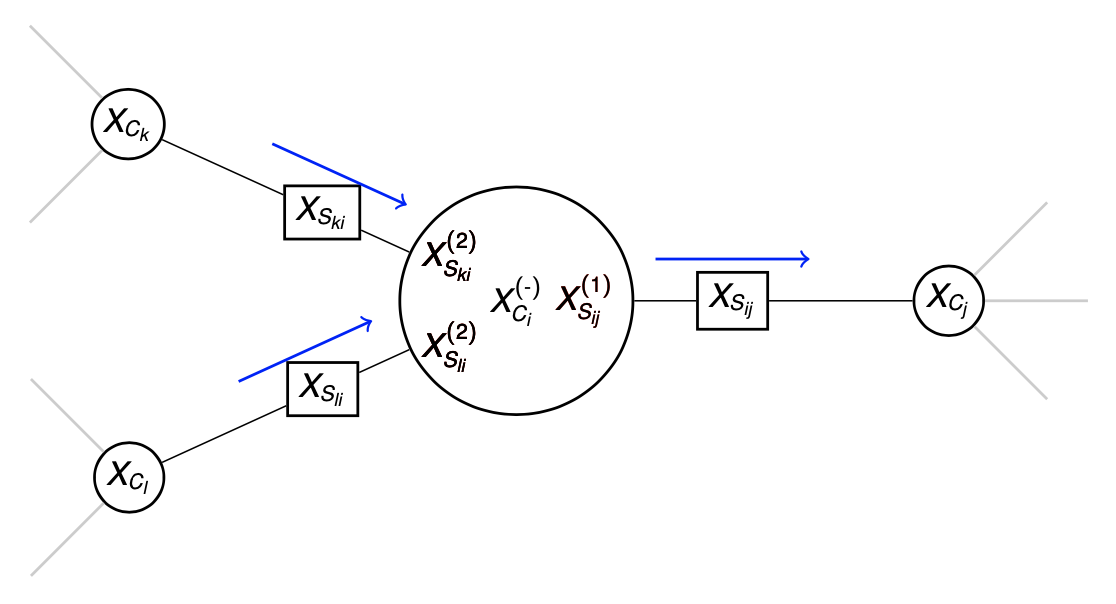
\includegraphics[width=10cm]{img/img10.png}
    \end{figure}  
\end{remark}

\begin{definition}{\textbf{(Shafer-Shenopy)}}
    We have the following formula of the message:
    \begin{equation*}
    \begin{aligned}
        M_{i\rightarrow j}(X^{(2)}_{S_{ij}}) &= \sum_{ X^{(-)}_{C_i}, \brackc{X^{(2)}_{S_{ki}} }, S^{(+)}_{S_{ij}} } f_i\bracka{X^{(-)}_{C_i}, \brackc{X^{(2)}_{S_{ki}} }, S^{(+)}_{S_{ij}} } f_{ij}\bracka{X^{(1)}_{S_{ij}}, X^{(2)}_{S_{ij}}} \prod_{k\in\operatorname{ne}(i)\backslash j} M_{k\rightarrow i}(X^{(2)}_{S_{ij}}) \\
        &= \sum_{X_{C_i}\backslash S_{ij}}f_i(X_{C_i}) \prod_{k\in\operatorname{ne}(i)\backslash j} M_{k\rightarrow i}(X_{S_{ij}}) \\
    \end{aligned}
    \end{equation*}
    The marginal distribution on cliques and separator are defined by:
    \begin{equation*}
    \begin{aligned}
        P(X_{C_i}) \propto f_i(X_{C_i})\prod_{k\in\operatorname{ne}(C_i)}M_{k\rightarrow i}(X_{S_{ki}}) \qquad P(X_{S_{ij}}) \propto M_{i\rightarrow j}(X_{S_{ij}})M_{j\rightarrow i}(X_{S_{ij}})
    \end{aligned}
    \end{equation*}
\end{definition}

\begin{remark}{\textbf{(Junction Tree Properties)}}
    The running intersection property and tree structure of the junction tree implies that local consistency between cliques and separator marginal gurantee global consistency: If we consider the distribution $q_i(X_{C_i})$ and $r_{ij}(X_{S_{ij}})$ are distribution such that:
    \begin{equation*}
        \sum_{X_{C_i\backslash S_{ij}}} q_i(X_{C_i}) = r_{ij}(X_{S_{ij}})
    \end{equation*}
    This implies that that joint distribution to be:
    \begin{equation*}
        P(\mathcal{X}) = \frac{\prod_{\text{cliques } i} q_i(X_{C_i})}{\prod_{\text{separator } (ij)} r_{ij}(X_{S_{ij}})}
    \end{equation*}
    As we have:
    \begin{equation*}
        q_i(X_{C_i}) = \sum_{\mathcal{X}\backslash X_{C_i}}P(\mathcal{X}) \qquad r_{ij}(X_{S_{ij}}) =  \sum_{\mathcal{X}\backslash X_{S_{ij}}}P(\mathcal{X})
    \end{equation*}
\end{remark}

\begin{definition}{\textbf{(Hugin Update)}}
    Let's start by initializing the variables to be:
    \begin{equation*}
        q_i(X_{C_i}) \propto f_i(X_{C_i}) \qquad r_{ij}(X_{S_{ij}}) \propto 1
    \end{equation*}
    A Hugin propagation update for $i\rightarrow j$ is given by:
    \begin{equation*}
        r^\text{new}_{ij} = \sum_{X_{C_i\backslash S_{ij}}}q_i(X_{C_i}) \qquad q^\text{new}_j(X_{C_j}) = q_j(X_{C_j})\frac{r^\text{new}_{ij}(X_{S_{ij}})}{r_{ij}(X_{S_{ij}})}
    \end{equation*}
    Setting the correct marginalization locally for the first update. For the second update, we change the $q$ based on the keeping the joint probability $P(\mathcal{X})$
\end{definition}


\section{Bayes and Gaussian Processes}

\subsection{Bayes Method}

\begin{remark}{\textbf{(Recap of Bayes)}}
    Model have a parameter $\theta_m$ that specify the probability of data $P(\mathcal{D}|\theta_m, m)$. If the model is known, learning $\theta_m$ means finding a posterior or point estimate. 
    \begin{itemize}
        \item What if we want to learn the type of model too ?
        \item Can we combine the model into a single \correctquote{supermodel} with a composite parameters ? 
        \item We can separate the model selection step: $P(\theta_m,m | \mathcal{D}) = P(\theta_m|m,\mathcal{D})P(m|\mathcal{D})$
    \end{itemize}
\end{remark}

\begin{definition}{\textbf{(Neyman-Peason Hypothesis Testing)}}
    For nested model, starting with simpliest model with $m=1$, comparing null hypothesis $m$ to its alternate $m+1$ and repeat until $m+1$ is rejected. Note that this tests only exact when it is asympototic in data number. Finally, it is conservative as it is asymmetric by design.
\end{definition}

\begin{definition}{\textbf{(Likelihood Validation)}}
    Partition data into disjoint training and validation set, where $D = D_\text{tr}\cup D_\text{valid}$. Then, we choose a model with greatest $P(D_\text{valid} | \theta^\text{ML}_m)$ where:
    \begin{equation*}
        \theta^\text{ML}_m = \argmax{\theta}P(D_\text{tr}|\theta)
    \end{equation*}
    or if we are able to find $P(D_\text{valid}|D_\text{train}, m)$. 
    \begin{itemize}
        \item This model is consistent and select the most useful model even if they are incorrect. 
        \item It may be biased toward a simpler models and gives a high-variance. 
        \item We can use cross-validation is used with multiple partition and average likelihood. 
    \end{itemize}
\end{definition}

\begin{definition}{\textbf{(Baysian Model Selection)}}
    We would like to choose a model $P(m|\mathcal{D})$  where consistent as it is a probability principle if true model is in the set. 
    \begin{itemize}
        \item However, it might be a problem of assumed prior. Finally, the posterior can weights models for combined prediction. 
        \item A model of class $m$ is a set of distributions parameterized by $\theta_m$. The model implies the prior over parameters as the posterior of the parameter:
        \begin{equation*}
            P(\theta_m | \mathcal{D}, m) = \frac{P(\mathcal{D}|\theta_m,m)P(\theta_m|m)}{P(\mathcal{D}|m)} \quad \text{ where } \quad 
        \end{equation*}
        where $P(\mathcal{D}|m)$ is the Baysian evidence for model $m$, where the ratio is known as Bayes factor:
        \begin{equation*}
            \frac{P(\mathcal{D}|m)}{P(\mathcal{D}|m')} = \frac{P(m|\mathcal{D})}{P(m'|\mathcal{D})}\frac{P(m')}{P(m)}
        \end{equation*}
        \item This is linked to Occam's razor where: the model that are \emph{too complex} can generate many data but they can be unlikely to generate a particular dataset. The model that are \emph{too simple} can't generate the data. 
    \end{itemize}
\end{definition}

\begin{remark}{\textbf{(Conjugate Prior)}}
    We will recall the use of exponential model. Suppose, we have $P(\mathcal{D}|\boldsymbol \theta_m,m)$ is member of the exponential family, where we can see that:
    \begin{equation*}
        P(\mathcal{D}|\boldsymbol \theta_m, m) = \prod^N_{i=1}P(\boldsymbol x_i | \boldsymbol \theta_m, m) = \prod^N_{i=1}\exp\bracka{\boldsymbol s(\boldsymbol x_i)^T\boldsymbol \theta_m - A(\boldsymbol \theta_m)}
    \end{equation*}
    Please note that $\boldsymbol A(\boldsymbol \theta_m)$ is the normalizing factor as it is (recall exponential family of the form in previous course) equal to $\ln(g(\boldsymbol \theta_m))$. Consider the prior conjugate to be:
    \begin{equation*}
        P(\boldsymbol \theta | m) = \frac{1}{Z(s_p, n_p)}\exp\bracka{\boldsymbol s_p^T\boldsymbol \theta_m - n_pA(\boldsymbol \theta_m)}
    \end{equation*}
    Then the posterior is equal to:
    \begin{equation*}
        P(\mathcal{D}, \boldsymbol \theta_m | m) = \frac{1}{Z(\boldsymbol s_p, p)}\exp\bracka{\bracka{\sum^N_{i=1}\boldsymbol s(\boldsymbol x_i) + \boldsymbol s_p}^T\boldsymbol \theta_m - (N+n_p)A(\boldsymbol \theta_m)}
    \end{equation*}
    One can show that:
    \begin{equation*}
        P(\mathcal{D}|m) = \int P(\mathcal{D}, \boldsymbol \theta_m | m) \dby\boldsymbol \theta_m = \frac{Z(\sum_i\boldsymbol s(\boldsymbol x_i) + \boldsymbol s_p, N + n_p)}{Z(\boldsymbol s_p, p)}
    \end{equation*}
\end{remark}

\begin{remark}{\textbf{(Laplace Approximation)}}
    To find $P(\mathcal{D} | m)$, we will have to perform the following integration:
    \begin{equation*}
        P(\mathcal{D}|m) = \int P(\mathcal{D}, \boldsymbol \theta_m | m)\dby\boldsymbol \theta_m
    \end{equation*}
    as the datasize $N$ grows, $\boldsymbol \theta$ becomes more concentrated as $P(\mathcal{D}, \boldsymbol \theta_m|m)\propto P(\boldsymbol \theta_m | \mathcal{D}, m)$ becomes concentrated on $\boldsymbol \theta_m^*$. Let's try to approximate the $P(\mathcal{D}, \boldsymbol \theta_m|m)$ to the second order around $\boldsymbol \theta_m^*$:
    \begin{equation*}
    \begin{aligned}
        \int P(\mathcal{D}, \boldsymbol \theta_m|m)\dby\boldsymbol \theta_m &= \int \exp(\log P(\mathcal{D}, \boldsymbol \theta_m|m))\dby \boldsymbol \theta_m \\
        &\approx\begin{aligned}[t]
            \int \exp\Big[ &\log P(\mathcal{D}, \boldsymbol \theta^*_m | m) + \underbrace{\nabla \log P(\mathcal{D}, \boldsymbol \theta_m^* | m)(\boldsymbol \theta_m - \boldsymbol \theta_m^*)}_{0} \\
            &+\frac{1}{2}(\boldsymbol \theta_m-\boldsymbol \theta_m^*)^T\underbrace{\nabla^2\log P(\mathcal{D}, \boldsymbol \theta_m^* | m)}_{-\boldsymbol A}(\boldsymbol \theta_m - \boldsymbol \theta_m^*) \Big]\dby\boldsymbol \theta_m 
        \end{aligned} \\
        &=\int P(\mathcal{D}, \boldsymbol \theta^*_m | m)\exp\brackb{-\frac{1}{2}(\boldsymbol \theta_m-\boldsymbol \theta_m^*)^T\boldsymbol A(\boldsymbol \theta_m - \boldsymbol \theta_m^*)}\dby\boldsymbol \theta \\
        &= P(\mathcal{D}|\boldsymbol \theta^*_m,m)P(\boldsymbol \theta^*_m|m)(2\pi)^{-d/2}\abs{\boldsymbol A}^{-1/2}
    \end{aligned}
    \end{equation*}
    This is approximating the posterior by a Gaussian, where an approximate that is asymmetrically correct. 
\end{remark}

\begin{definition}{\textbf{(Baysian Information Criterion)}}
    BIC can be obtained from Laplace approximate:
    \begin{equation*}
        \log P(\mathcal{D} | m) \approx \log P(\boldsymbol \theta^* | m) + \log P(\mathcal{D}|\boldsymbol \theta^*_m, m) + \frac{d}{2}\log 2\pi - \frac{1}{2}\log\abs{\boldsymbol A}
    \end{equation*}
    where we further have:
    \begin{equation*}
        \boldsymbol A = -\nabla^2\log P(\mathcal{D}, \boldsymbol \theta^*_m | m) = -\nabla^2\log P(\mathcal{D}|\boldsymbol \theta^*, m) -\nabla^2\log P(\boldsymbol \theta^*|m)
    \end{equation*}
    As $N=|D|\rightarrow\infty$ and $A\rightarrow N\boldsymbol A_0 + \text{const}$ for a fixed positive definite matrix $\boldsymbol A_0 = \brackd{-\nabla^2\log P(\boldsymbol x | \boldsymbol \theta^*, m)}$ as we have $\log\abs{N\boldsymbol A_0} = d\log N + \log\abs{\boldsymbol A_0}$. We will retain only the term that grows with $N$ to be:
    \begin{equation*}
        \log P(\mathcal{D} | m) \approx \log P(\mathcal{D}|\boldsymbol \theta^*_m, m) - \frac{d}{2}\log N
    \end{equation*}
\end{definition}

\begin{remark}{\textbf{(Properties BIC)}}
    Baysian Information Criterion has the following properties, as we have:
    \begin{itemize}
        \item Quick and Easy to compute. It doesn't depend on the prior as we can use ML to estimate instead of MAP estimate. 
        \item It is related to minimal description length. Given the assuption that in large sample limit, all parameter are well determined. But it negated multiple nodes (permuation of mixture of Gaussian).
    \end{itemize}
\end{remark}

\begin{definition}{\textbf{(Hyperparameter and Evidence Optimization)}}
    Need to choose between a family of continuous parameterized models:
    \begin{equation*}
        P(\mathcal{D} | \boldsymbol \eta) = \int P(\mathcal{D} | \boldsymbol \theta)P(\boldsymbol \theta | \boldsymbol \eta) \dby \boldsymbol \theta
    \end{equation*}
    We can perform an ascending on gradient in: the exact evidence, approximate evidence (Laplace, BIC) or free-energy based on the evidence (variational Bayes). Performing the hyper-prior on $\boldsymbol \eta$, which we can sample its posterior via MCMC as:
    \begin{equation*}
        P(\boldsymbol \eta | \mathcal{D}) = \frac{P(\mathcal{D}|\boldsymbol \eta)P(\boldsymbol \eta)}{P(\mathcal{D})}
    \end{equation*}
\end{definition}

\subsection{Linear Regression/Gaussian Process}

\begin{definition}{\textbf{(Linear Regression)}}
    We consider the following graphical model as:
    \begin{figure}[H]
        \centering
        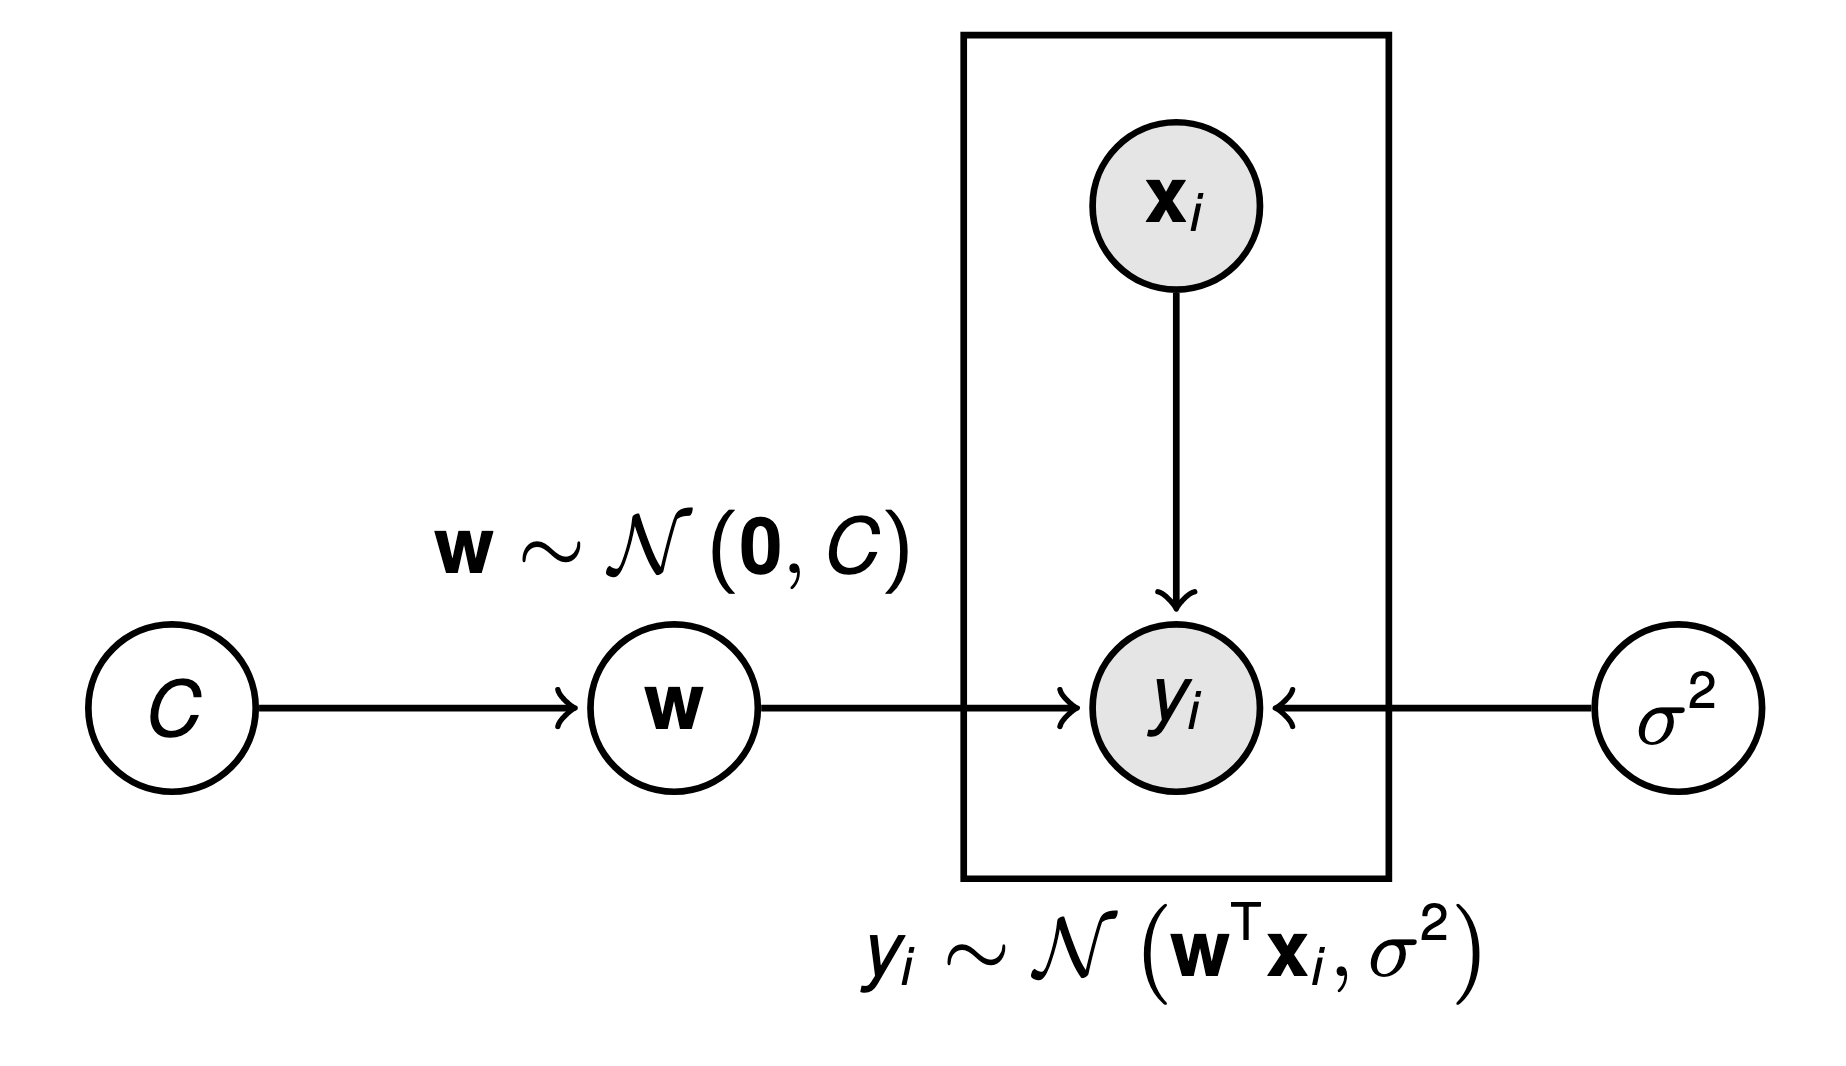
\includegraphics[width=8cm]{img/img11.png}
    \end{figure}  
    To find the hyperparameters, we can see that:
    \begin{equation*}
        P(\brackc{y_i}^N_{i=1} | \brackc{\boldsymbol x_i}^N_{i=1}, \boldsymbol C, \sigma^2) = \int P(\brackc{y_i}^N_{i=1} | \brackc{\boldsymbol x_i}^N_{i=1}, \boldsymbol w, \sigma^2)P(\boldsymbol w | \boldsymbol C)\dby \boldsymbol w
    \end{equation*}
    Maximizing the value of $\boldsymbol C$ and $\sigma^2$.
\end{definition}

\begin{proposition}
    The update rule for the parameter $\boldsymbol \theta = \brackc{\boldsymbol C, \boldsymbol \sigma^2}$ is:
    \begin{equation*}
    \begin{aligned}
        &\frac{\partial}{\partial \boldsymbol \theta} \log \mathcal{E}(\boldsymbol C, \sigma^2) = \frac{1}{2}\operatorname{Tr}\brackb{(\boldsymbol C - \boldsymbol \Sigma_w - \bar{\boldsymbol w}\bar{\boldsymbol w}^T)\frac{\partial}{\partial \boldsymbol \theta} \boldsymbol C^{-1}} \\
        &\frac{\partial}{\partial \sigma^2}\log\mathcal{E}(\boldsymbol C,\sigma^2) = \frac{1}{\sigma^2}\bracka{-N + \operatorname{Tr}[\boldsymbol I - \boldsymbol \Sigma_w\boldsymbol C^{-1}] + \frac{1}{\sigma^2}(\boldsymbol Y - \boldsymbol X^T\bar{\boldsymbol w})^T(\boldsymbol Y - \boldsymbol X^T\bar{\boldsymbol w})}
    \end{aligned}
    \end{equation*}
\end{proposition}

\begin{proof}
    We can see that the posterior of $P\bracka{\boldsymbol w \left| \brackc{y_i}^N_{i=1}, \brackc{\boldsymbol x_i}^N_{i=1}, \boldsymbol C,\sigma^2\right.}$. We can see that the posterior on $\boldsymbol w$ is normal with:
    \begin{equation*}
        \Sigma_{\boldsymbol w} = \bracka{\frac{\boldsymbol X\boldsymbol X^T}{\sigma^2} + \boldsymbol C^{-1}}^{-1} \qquad \bar{\boldsymbol w} = \boldsymbol \Sigma_{\boldsymbol w}\frac{\boldsymbol X\boldsymbol Y}{\sigma^2}
    \end{equation*}
    This follows from the eariler works. Now, we can consider terms inside the exponential of the joint distributions $P(\boldsymbol Y | \boldsymbol X, \boldsymbol w, \sigma^2)P(\boldsymbol w | \boldsymbol C)$:
    \begin{equation*}
    \begin{aligned}
        -\frac{1}{2\sigma^2}\boldsymbol Y^T\boldsymbol Y &+ \frac{1}{\sigma^2}\boldsymbol w^T\boldsymbol X\boldsymbol Y - \frac{1}{2}\Big[ \boldsymbol w^T\boldsymbol \Sigma_w^{-1}\boldsymbol w \Big] \\
        &=-\frac{1}{2\sigma^2}\boldsymbol Y^T\boldsymbol Y - \frac{1}{2}\brackc{\boldsymbol w^T\boldsymbol \Sigma^{-1}_w\boldsymbol w^T - \frac{2}{\sigma^2}\boldsymbol w^T\boldsymbol \Sigma_w\boldsymbol \Sigma^{-1}_w\boldsymbol X\boldsymbol Y} \\
        &=\begin{aligned}[t]
            -\frac{1}{2\sigma^2}\boldsymbol Y^T\boldsymbol Y &- \frac{1}{2}\brackc{\boldsymbol w^T\boldsymbol \Sigma^{-1}_w\boldsymbol w^T - \frac{2}{\sigma^2}\boldsymbol w^T\boldsymbol \Sigma_w\boldsymbol \Sigma^{-1}_w\boldsymbol X\boldsymbol Y + \frac{1}{\sigma^4}\boldsymbol Y^T\boldsymbol X^T\boldsymbol \Sigma^T_w\boldsymbol \Sigma^{-1}_w\boldsymbol \Sigma^T_w\boldsymbol X\boldsymbol Y} \\
            &+ \frac{1}{2\sigma^4}\boldsymbol Y^T\boldsymbol X^T\boldsymbol \Sigma^T_w\boldsymbol X\boldsymbol Y
        \end{aligned} \\
        &= -\frac{1}{2\sigma^2}\boldsymbol Y^T\boldsymbol Y + \frac{1}{2\sigma^4}\boldsymbol Y^T\boldsymbol X^T\boldsymbol \Sigma^T_w\boldsymbol X\boldsymbol Y -\frac{1}{2}\bracka{\boldsymbol w - \frac{1}{\sigma^2}\boldsymbol \Sigma_w\boldsymbol X\boldsymbol Y}^T\boldsymbol \Sigma^{-1}_w\bracka{\boldsymbol w - \frac{1}{\sigma^2}\boldsymbol \Sigma_w\boldsymbol X\boldsymbol Y}
    \end{aligned}
    \end{equation*}
    If we consider the quadratic terms, and the integration over it we have:
    \begin{equation*}
        \int \exp\brackc{-\frac{1}{2}\bracka{\boldsymbol w-\frac{1}{\sigma^2}\boldsymbol \Sigma_w\boldsymbol X\boldsymbol Y}^T\boldsymbol \Sigma^{-1}_w\bracka{\boldsymbol w - \frac{1}{\sigma^2}\boldsymbol \Sigma_w\boldsymbol X\boldsymbol Y}} \dby \boldsymbol w
    \end{equation*}
    This is the Gaussian integration, which it is a constant that we can ignore. This leads to the evidence to be (the normalizing factor can be easily found):
    \begin{equation*}
        \mathcal{E}(\boldsymbol C, \sigma^2) = \sqrt{\frac{\abs{2\pi\boldsymbol \Sigma_w}}{\abs{2\pi\sigma^2\boldsymbol I}\abs{2\pi\boldsymbol C}}}\exp\brackc{-\frac{1}{2}\boldsymbol Y^T\bracka{\frac{I}{\sigma^2} - \frac{\boldsymbol X^T\boldsymbol \Sigma_w\boldsymbol X}{\sigma^4}}\boldsymbol Y}
    \end{equation*}
    Now, let's consider the derivative to be, starting with the value of $\boldsymbol C$, we can see that the relevant values:
    \begin{equation*}
    \begin{aligned}
        \frac{1}{2}\frac{\partial}{\partial \boldsymbol \theta}\log\abs{\boldsymbol \Sigma_w} &- \frac{1}{2}\frac{\partial}{\partial \boldsymbol \theta}\log\abs{\boldsymbol C} + \frac{1}{2}\frac{\partial}{\partial \boldsymbol  \theta}\frac{\boldsymbol Y^T\boldsymbol X^T\boldsymbol \Sigma_w\boldsymbol X\boldsymbol Y}{\sigma^4} \\
        &= -\frac{1}{2}\frac{\partial}{\partial \boldsymbol \theta}\abs{\boldsymbol \Sigma_w^{-1}} + \frac{1}{2}\frac{\partial}{\partial \boldsymbol  \theta}\log\abs{\boldsymbol C^{-1}} + \frac{1}{2}\frac{\partial}{\partial \boldsymbol  \theta}\frac{\boldsymbol Y^T\boldsymbol X^T\boldsymbol \Sigma_w\boldsymbol X\boldsymbol Y}{\sigma^4} \\ 
        &= -\frac{1}{2}\operatorname{Tr}\bracka{\Sigma_w\frac{\partial \boldsymbol C^{-1}}{\partial \boldsymbol \theta}} + \frac{1}{2}\operatorname{Tr}\bracka{\boldsymbol C\frac{\partial \boldsymbol C^{-1}}{\partial \boldsymbol \theta}} + \frac{1}{2\sigma^4}\operatorname{Tr}\bracka{\boldsymbol X\boldsymbol Y\boldsymbol Y^T\boldsymbol X^T\frac{\partial \boldsymbol \Sigma^{-1}_w}{\partial \boldsymbol \theta}} \\
        &=\begin{aligned}[t]
            -\frac{1}{2}\operatorname{Tr}&\bracka{\Sigma_w\frac{\partial \boldsymbol C^{-1}}{\partial \boldsymbol \theta}} + \frac{1}{2}\operatorname{Tr}\bracka{\boldsymbol C\frac{\partial \boldsymbol C^{-1}}{\partial \boldsymbol \theta}} \\
            &- \frac{1}{2\sigma^4}\operatorname{Tr}\bracka{\boldsymbol X\boldsymbol Y\boldsymbol Y^T\boldsymbol X^T \boldsymbol \Sigma^{-1}_w\frac{\partial}{\partial \boldsymbol \theta}\brackb{ \frac{\boldsymbol X\boldsymbol X^T}{\sigma^2} + \boldsymbol C^{-1}}\boldsymbol \Sigma_w} \\
        \end{aligned}  \\
        &=\begin{aligned}[t]
            -\frac{1}{2}\operatorname{Tr}&\bracka{\Sigma_w\frac{\partial \boldsymbol C^{-1}}{\partial \boldsymbol \theta}} + \frac{1}{2}\operatorname{Tr}\bracka{\boldsymbol C\frac{\partial \boldsymbol C^{-1}}{\partial \boldsymbol \theta}} \\
            &- \frac{1}{2\sigma^4}\operatorname{Tr}\bracka{\boldsymbol X\boldsymbol Y\boldsymbol Y^T\boldsymbol X^T \boldsymbol \Sigma_w\brackb{ \frac{\partial\boldsymbol C^{-1}}{\partial \boldsymbol \theta} }\boldsymbol \Sigma_w} \\
        \end{aligned}  \\
        &=\begin{aligned}[t]
            -\frac{1}{2}\operatorname{Tr}&\bracka{\Sigma_w\frac{\partial \boldsymbol C^{-1}}{\partial \boldsymbol \theta}} + \frac{1}{2}\operatorname{Tr}\bracka{\boldsymbol C\frac{\partial \boldsymbol C^{-1}}{\partial \boldsymbol \theta}} \\
            &- \frac{1}{2}\operatorname{Tr}\bracka{\frac{\boldsymbol Y^T\boldsymbol X^T \boldsymbol \Sigma_w}{\sigma^2}\brackb{ \frac{\partial\boldsymbol C^{-1}}{\partial \boldsymbol \theta} }\frac{\boldsymbol \Sigma_w\boldsymbol X\boldsymbol Y}{\sigma^2}} \\
        \end{aligned}  \\
        &=\begin{aligned}[t]
            -\frac{1}{2}\operatorname{Tr}&\bracka{\Sigma_w\frac{\partial \boldsymbol C^{-1}}{\partial \boldsymbol \theta}} + \frac{1}{2}\operatorname{Tr}\bracka{\boldsymbol C\frac{\partial \boldsymbol C^{-1}}{\partial \boldsymbol \theta}} - \frac{1}{2}\operatorname{Tr}\bracka{\bar{\boldsymbol w}\bar{\boldsymbol w}^T\brackb{ \frac{\partial\boldsymbol C^{-1}}{\partial \boldsymbol \theta} }} \\
        \end{aligned} 
    \end{aligned}
    \end{equation*}
    Please recall the derivative of the inverse, and we finish the proof. Now consider the derivative of the evidence with respected to $S = \sigma^2$, 
    \begin{equation*}
    \begin{aligned}
        \underbrace{\frac{1}{2}\frac{\partial}{\partial S}\log\abs{\boldsymbol \Sigma_w}}_{\circled{1}} &- \frac{N}{2}\frac{\partial }{\partial S} \log S -\frac{1}{2}\frac{\partial }{\partial S}\frac{\boldsymbol Y^T\boldsymbol Y}{S} + \underbrace{\frac{1}{2}\frac{\partial }{\partial S}\frac{\boldsymbol Y^T\boldsymbol X^T\boldsymbol \Sigma_w\boldsymbol X\boldsymbol Y}{S^2} }_{\circled{2}}
    \end{aligned}
    \end{equation*}
    And we have the following derivative for $\circled{1}$, as we have:
    \begin{equation*}
    \begin{aligned}
        \frac{\partial}{\partial S}\log\abs{\boldsymbol \Sigma_w} &= -\frac{\partial}{\partial S}\log\abs{\boldsymbol \Sigma_w^{-1}} \\
        &=- \operatorname{Tr}\bracka{\boldsymbol \Sigma_w\frac{\partial \boldsymbol \Sigma_w^{-1}}{\partial S}} \\
        &=- \operatorname{Tr}\bracka{\boldsymbol \Sigma_w\frac{\partial}{\partial S}\brackb{\frac{\boldsymbol X\boldsymbol X^T}{S} + \boldsymbol C^{-1}}} \\
        &=\frac{1}{S^2} \operatorname{Tr}\bracka{\boldsymbol \Sigma_w\boldsymbol X\boldsymbol X^T} \\
    \end{aligned}
    \end{equation*}
    For for the equation $\circled{2}$, we have:
    \begin{equation*}
    \begin{aligned}
        \frac{\partial }{\partial S}\frac{\boldsymbol Y^T\boldsymbol X^T\boldsymbol \Sigma_w\boldsymbol X\boldsymbol Y}{S^2} &= \boldsymbol Y^T\boldsymbol X^T\boldsymbol \Sigma_w\boldsymbol X\boldsymbol Y\frac{\partial }{\partial S}\frac{1}{S^2} + \frac{1}{S^2}\frac{\partial }{\partial S}\boldsymbol Y^T\boldsymbol X^T\boldsymbol \Sigma_w\boldsymbol X\boldsymbol Y \\
        &= -2\frac{\boldsymbol Y^T\boldsymbol X^T\boldsymbol \Sigma_w\boldsymbol X\boldsymbol Y}{S^3} + \frac{1}{S}\boldsymbol Y^T\boldsymbol X^T\boldsymbol \Sigma_w\frac{\partial }{\partial S}\brackb{\frac{\boldsymbol X\boldsymbol X^T}{S} + C^{-1}}\frac{1}{S}\boldsymbol \Sigma_w\boldsymbol X\boldsymbol Y \\
        &= -2\boldsymbol Y^T\boldsymbol X^T\bar{\boldsymbol w} + \bar{\boldsymbol w}^T \bracka{\boldsymbol X\boldsymbol X^T}\bar{\boldsymbol w}
    \end{aligned}
    \end{equation*}
    Combining them and we have:
    \begin{equation*}
    \begin{aligned}
        \frac{1}{2S}\Bigg( &\frac{1}{S}\operatorname{Tr}\bracka{\boldsymbol \Sigma_w\boldsymbol X\boldsymbol X^T} - N + \frac{1}{S}\boldsymbol Y^T\boldsymbol Y - \frac{1}{S}2\boldsymbol Y^T\boldsymbol X^T\bar{\boldsymbol w} + \frac{1}{S}\bar{\boldsymbol w}^T \Sigma_w\bracka{\boldsymbol X\boldsymbol X^T}\bar{\boldsymbol w} \Bigg) \\
        &= \frac{1}{2S}\bracka{-N + \frac{1}{S}\operatorname{Tr}\bracka{ \boldsymbol \Sigma_w\boldsymbol X\boldsymbol X^T} + \frac{1}{S} (\boldsymbol Y - \boldsymbol X^T\bar{\boldsymbol w})^T(\boldsymbol Y - \boldsymbol X^T\bar{\boldsymbol w}) }
    \end{aligned}
    \end{equation*}
    Please note that there are some differeces between this and the final proof, which we can't get it but most of them seem correct already
\end{proof}

\begin{definition}{\textbf{(Automatic Relevence Determination (ARD))}}
    The most common form of evidence optimization with $\boldsymbol C^{-1} = \operatorname{diag}(\boldsymbol \alpha)$ and the optimize $\{\alpha_i\}$ setting the gradient to $0$, which we now have:
    \begin{equation*}
        \alpha^\text{new}_i = \frac{1-\alpha_i[\boldsymbol \Sigma_n]_{ii}}{\bar{w}_i^2} \qquad (\alpha^2)^\text{new} = \frac{(\boldsymbol Y - \boldsymbol X^T\bar{\boldsymbol w})^T(\boldsymbol Y - \boldsymbol X^T\bar{\boldsymbol w})}{N - \sum_i (1 - [\boldsymbol \Sigma_w]_{ii}\alpha_i)}
    \end{equation*}
    During the optimization, there are $2$ possible scenario for $\boldsymbol \alpha$:
    \begin{itemize}
        \item $\alpha_i\rightarrow\infty$ where the weight $\alpha_i = 0$
        \item $\alpha_i$ is finite and so $w_i = \arg\max P(w_i | \boldsymbol X, \boldsymbol Y, \alpha_i)$
    \end{itemize}
    This is called Automatic Relevence Determination (ARD), which yields space solution that improve ML regression (like LASSA) This Evidence maximization is called ML likelihood or ML-2. 
\end{definition}

\begin{definition}{\textbf{(Prediction Averaging)}}
    We integrate out the parameter, where we have the density estimation:
    \begin{equation*}
        P(\boldsymbol x | \mathcal{D}, m) = \int P(\boldsymbol x | \boldsymbol \theta, m)P(\boldsymbol \theta | \mathcal{D}, m)\dby \boldsymbol \theta
    \end{equation*} 
    Or, perform the prediction:
    \begin{equation*}
        P(y | \boldsymbol x, \mathcal{D}, m) =\int P(y | \boldsymbol x, \theta, m)P(\theta|\mathcal{D}, m)\dby\boldsymbol \theta
    \end{equation*}
    This kind of prediction might resists overfitting with infintely complex model as this can be called Baysian non-parametric, which leads to Gaussian Process.
\end{definition}

\begin{proposition}{\textbf{(Prediction)}}
    Given a new input vector $\boldsymbol x$, the predicted output $y$ is given by:
    \begin{equation*}
        y | \boldsymbol x \sim \mathcal{N}(\bar{\boldsymbol w}^T\boldsymbol x, \boldsymbol x^T\boldsymbol \Sigma_w\boldsymbol x + \sigma^2)
    \end{equation*}
    This comes from the linear Gaussian model. The variance $\boldsymbol x^T\boldsymbol \Sigma_w\boldsymbol x$ that comes from the uncertainty of $\boldsymbol w$.
\end{proposition}

\begin{remark}{\textbf{(Observation on Joint Distribution)}}
    Consider the joint probability between $y_1,\dots,y_N$ and $\boldsymbol x_1, \dots,\boldsymbol x_N$, and noisy prediction with variance $\tau^2$, we can see that the mean and the covariances are:
    \begin{equation*}
    \begin{aligned}
        &\mathbb{E}[y_i] = \mathbb{E}[\boldsymbol w^T\boldsymbol x_i] = 0 \\
        &\mathbb{E}[(y_i-\bar{y}_i)^2] = \mathbb{E}[(\boldsymbol x_i^T\boldsymbol w)(\boldsymbol w^T\boldsymbol x_i)] + \sigma^2 = \tau^2\boldsymbol x_i^T\boldsymbol x_i + \sigma^2 \\
        &\mathbb{E}[(y_i-\bar{y}_i)(y_j-\bar{y}_j)] = \mathbb{E}[(\boldsymbol x_i^T\boldsymbol w)(\boldsymbol w^T\boldsymbol x_j)] = \tau^2 \boldsymbol x_i^T\boldsymbol x_j
    \end{aligned}
    \end{equation*}
    So the leads to the following joint distributions:
    \begin{equation*}
        \left.\begin{bmatrix}
            y_1 \\ y_2 \\ \vdots \\ y_N
        \end{bmatrix}\right| \boldsymbol x_1,\dots,\boldsymbol x_N \sim \mathcal{N}\bracka{\begin{bmatrix}
            0 \\ 0 \\ \vdots \\ 0
        \end{bmatrix}, \begin{bmatrix}
            \tau^2\boldsymbol x_1^T\boldsymbol x_1 + \sigma^2 & \tau^2\boldsymbol x_1^T\boldsymbol x_2 & \cdots & \tau^2\boldsymbol x_1^T\boldsymbol x_N \\
            \tau^2\boldsymbol x_2^T\boldsymbol x_1 & \tau^2\boldsymbol x_2^T\boldsymbol x_2 + \sigma^2 & \cdots & \tau^2\boldsymbol x_2^T\boldsymbol x_N \\
            \vdots & \vdots & \ddots & \vdots \\
            \tau^2\boldsymbol x_N^T\boldsymbol x_1 & \tau^2\boldsymbol x_N^T\boldsymbol x_2 & \cdots & \tau^2\boldsymbol x_N^T\boldsymbol x_N + \sigma^2  \\
        \end{bmatrix}}
    \end{equation*}
    If we were to consider adding the test input vector $\boldsymbol x$ and test vector $y$, we have:
    \begin{equation*}
        \left.\begin{bmatrix}
            \boldsymbol Y^T \\ y
        \end{bmatrix}\right| \boldsymbol X, \boldsymbol x \sim \mathcal{N}\bracka{\begin{bmatrix}
            \boldsymbol 0 \\ 0
        \end{bmatrix}, \begin{bmatrix}
            \tau \boldsymbol X^T\boldsymbol X + \sigma^2\boldsymbol I & \tau^2 \boldsymbol X^T\boldsymbol x \\
            \tau^2 \boldsymbol x^T\boldsymbol X & \tau \boldsymbol x^T\boldsymbol x + \sigma^2
        \end{bmatrix}} = \mathcal{N}\bracka{\begin{bmatrix}
            \boldsymbol 0 \\ 0
        \end{bmatrix}, \begin{bmatrix}
            \tilde{\boldsymbol K}_{XX} & \tilde{\boldsymbol K}_{Xx} \\
            \tilde{\boldsymbol K}_{xX} & \tilde{\boldsymbol K}_{xx} \\
        \end{bmatrix}}
    \end{equation*}
    By the linear Gaussian model, we are given, the following conditional
    \begin{equation*}
    \begin{aligned}
        y | \boldsymbol Y, \boldsymbol X, \boldsymbol x &\sim \mathcal{N}\Big( \tilde{\boldsymbol K}_{xX}\tilde{\boldsymbol K}_{XX}^{-1}\boldsymbol Y^T, \ \tilde{\boldsymbol K}_{xx} - \tilde{\boldsymbol K}_{xX}\tilde{\boldsymbol K}_{XX}^{-1}\tilde{\boldsymbol K}_{Xx} \Big) \\
        &\sim \mathcal{N}\Big( \tau^2\boldsymbol x^T\boldsymbol X(\tau^2 \boldsymbol X^T\boldsymbol X + \sigma^2 \boldsymbol I)^{-1}\boldsymbol Y^T, \ \tau^2\boldsymbol x^T\boldsymbol x + \sigma^2 - \tau^2\boldsymbol x^T\boldsymbol X(\tau^2\boldsymbol X^T\boldsymbol X + \sigma^2)^{-1}\tau^2\boldsymbol X^T\boldsymbol x \Big) \\
        &\sim \mathcal{N}\bracka{ \boldsymbol x^T\frac{1}{\sigma^2} \boldsymbol \Sigma\boldsymbol X\boldsymbol Y^T, \boldsymbol x^T\boldsymbol \Sigma\boldsymbol x + \sigma^2 }
    \end{aligned}
    \end{equation*}
    where $\boldsymbol \Sigma = (\frac{1}{\sigma^2}\boldsymbol X\boldsymbol X^T + \frac{1}{\tau^2}\boldsymbol I)^{-1}$. The derivation comes from the Woodbury identity. 
\end{remark}

\begin{remark}{\textbf{(Non-Linear Regression)}}
    We consider the mapping $\boldsymbol x\mapsto \boldsymbol \phi(\boldsymbol x)$, the regression:
    \begin{equation*}
        \boldsymbol Y | \boldsymbol X \sim \mathcal{N}(\boldsymbol 0_N, \tau^2 \boldsymbol \Phi^T\boldsymbol \Phi + \sigma^2\boldsymbol I_N)
    \end{equation*}
    where $i$-th column of matrix $\boldsymbol \Phi$ is $\boldsymbol \phi(\boldsymbol x_i)$. Now we have the following prediction:
    \begin{equation*}
        \boldsymbol y | \boldsymbol Y, \boldsymbol X, \boldsymbol x \sim \mathcal{N}(\tilde{\boldsymbol K}_{xX}\tilde{\boldsymbol K}_{XX}^{-1}\boldsymbol Y^T, \ \tilde{\boldsymbol K}_{xx}-\tilde{\boldsymbol K}_{xX}\tilde{\boldsymbol K}^{-1}_{XX}\tilde{\boldsymbol K}_{Xx})
    \end{equation*}
    where we have:
    \begin{equation*}
        \tilde{\boldsymbol K}_{XX} = \tau^2\boldsymbol \Phi^T\boldsymbol \Phi + \sigma^2\boldsymbol I \qquad \tilde{\boldsymbol K}_{Xx} = \tau^2\boldsymbol \Phi^T\boldsymbol \phi(\boldsymbol x) \qquad \tilde{\boldsymbol K}_{xx} = \tau^2\boldsymbol \phi(\boldsymbol x)^T\boldsymbol \phi(\boldsymbol x) + \sigma^2
    \end{equation*}
\end{remark}

\begin{remark}{\textbf{(Kernel Vector)}}
    Define a covariance kernel function $\tilde{K}:\mathbb{X}\times \mathbb{X}\rightarrow \mathbb{R}$ if $\boldsymbol x, \boldsymbol x' \in \mathbb{X}$ are $2$ inputs vectors with corresponding output $y$ and $y'$, then we have:
    \begin{equation*}
        \tilde{K}(\boldsymbol x,\boldsymbol x') = \operatorname{Cov}[y, y'] = \mathbb{E}[yy'] - \mathbb{E}[y]\mathbb{E}[y']
    \end{equation*}
    In non-linear regression problem we have $\tilde{K}(\boldsymbol x, \boldsymbol x') =\tau^2\boldsymbol \phi(\boldsymbol x)^T\boldsymbol \phi(\boldsymbol x') + \sigma^2\delta[\boldsymbol x = \boldsymbol x']$, where the prediction depends on $\tilde{\boldsymbol K}(\boldsymbol x, \boldsymbol x')$ rather than its feature map $\boldsymbol \phi(\boldsymbol x)$ and so, we have:
    \begin{equation*}
        \boldsymbol Y | \boldsymbol X, \tilde{\boldsymbol K} \sim \mathcal{N}(\boldsymbol 0_N, \tilde{\boldsymbol K}_{XX})
    \end{equation*}
    To perform a prediction, as we have:
    \begin{equation*}
        \boldsymbol y | \boldsymbol Y, \boldsymbol X, \boldsymbol x \sim \mathcal{N}(\tilde{\boldsymbol K}_{xX}\tilde{\boldsymbol K}_{XX}^{-1}\boldsymbol Y^T, \ \tilde{\boldsymbol K}_{xx}-\tilde{\boldsymbol K}_{xX}\tilde{\boldsymbol K}^{-1}_{XX}\tilde{\boldsymbol K}_{Xx})
    \end{equation*}
    where $\brackb{\tilde{\boldsymbol K}_{XX}}_{ij} = \tilde{\boldsymbol K}(\boldsymbol x_i, \boldsymbol x_j)$, $\brackb{\tilde{\boldsymbol K}_{Xx}}_i = \tilde{\boldsymbol K}(\boldsymbol x_i, \boldsymbol X)$ and $\tilde{K}_{xx} = \tilde{\boldsymbol K}(\boldsymbol x, \boldsymbol x)$, now we can have the kernel function solely without the use of the feature map. 
\end{remark}

\begin{definition}{\textbf{(Gaussian Process)}}
    Let $f(\boldsymbol x)$ be random variable indexed by $\boldsymbol x$, then drawn from the whole GP, which is a random function $f:\mathbb{X}\rightarrow \mathbb{R}$ where:
    \begin{equation*}
        f(\cdot) \sim \mathcal{GP}(m(\cdot), k(\cdot, \cdot))
    \end{equation*}
    It is defiend such that the finite list of points $\brackc{\boldsymbol x_1,\dots,\boldsymbol x_N}$. The joint distributions of the function value $f=[f(\boldsymbol x_1),\dots,f(\boldsymbol x_N)]^T$ as we have $\boldsymbol f | \boldsymbol X, \boldsymbol K \sim \mathcal{N}(\boldsymbol m, \boldsymbol K_{XX})$ with the following parameters:
    \begin{equation*}
        [\boldsymbol K_{XX}]_{ij} = K(\boldsymbol x_i, \boldsymbol x_j) \qquad [\boldsymbol m]_i = \boldsymbol m(\boldsymbol x_i)
    \end{equation*}
\end{definition}

\begin{remark}{\textbf{(Properties of Gaussian Process + Bayes Theorem)}}
    If we assume the random function is dranw from GP prior $f(\cdot) \sim \mathcal{GP}(\boldsymbol 0, K(\cdot, \cdot))$. Observation $y_i$ taken to be noisy version of latent function $f(\boldsymbol x_i)$ where we have:
    \begin{equation*}
        \boldsymbol y_i | \boldsymbol x_i, f(\cdot) \sim \mathcal{N}(y(\boldsymbol x_i), \sigma^2)
    \end{equation*}
    The we have the following quantities:
    \begin{itemize}
        \item The latent $f$ is also Gaussian process:
        \begin{equation*}
            f(\cdot) | \boldsymbol X, \boldsymbol Y \sim \mathcal{GP}\Big( \boldsymbol K_{\cdot X}(\boldsymbol K_{XX} + \sigma^2I)^{-1}\boldsymbol Y^T, \ K(\cdot,\cdot) - K_{\cdot X}(\boldsymbol K_{XX} + \sigma^2\boldsymbol I)^{-1}\boldsymbol K_{X\cdot} \Big)
        \end{equation*}
        \item This is given multivariate Gaussian likelihood:
        \begin{equation*}
            P(\boldsymbol Y | \boldsymbol X) = \abs{2\pi(\boldsymbol K_{xx} + \sigma^2\boldsymbol I)^{-1/2}}\exp\bracka{-\frac{1}{2}\boldsymbol Y(\boldsymbol K_{xx} + \sigma^2\boldsymbol I)\boldsymbol Y^T}
        \end{equation*}
        \item The posterior of $f$ with observation noise, as we have:
        \begin{equation*}
            y | \boldsymbol X, \boldsymbol Y, \boldsymbol x \sim \mathcal{N}(\mathbb{E}[f(\boldsymbol x) | \boldsymbol X, \boldsymbol Y], \operatorname{Var}[f(\boldsymbol x) | \boldsymbol X, \boldsymbol Y] + \sigma^2)
        \end{equation*}
    \end{itemize}
\end{remark}




\section{Support Vector Machine}

\subsection{Forming Problems}

\begin{definition}{\textbf{(Seperating Hyperplane)}}
    Let the dataset be $S = \brackc{(\boldsymbol x_i, y_i)}^m_{i=1} \in \mathbb{R}^n \times \brackc{-1, 1}$. The hyperplane is the set such that:
    \begin{equation*}
        \mathcal{H}_{\boldsymbol w, b} = \brackc{\boldsymbol x\in \mathbb{R}^n : \boldsymbol w^T\boldsymbol x + b = 0}
    \end{equation*}
\end{definition}

\begin{definition}{\textbf{(Linearly Separatable)}}
    The data are linearly separatable if there exists $\boldsymbol w \in \mathbb{R}^n$ and $b\in \mathbb{R}$ such that:
    \begin{equation*}
        y_i(\boldsymbol w^T\boldsymbol x_i + b) > 0
    \end{equation*}
    for $i=1,\dots,m$, which we call $\mathcal{H}_{\boldsymbol w, b}$ a separating hyperplane. Note that it is a strict inequality. 
\end{definition}

\begin{proposition}{\textbf{(Finding A distance from Plane)}}
    If $\mathcal{H}_{\boldsymbol w, b}$ is a hyperplane, we also define the distance from a point $\boldsymbol x$ to be:
    \begin{equation*}
        \frac{\boldsymbol w^T\boldsymbol x + b}{\norm{\boldsymbol w}}
    \end{equation*}
\end{proposition}
\begin{proof}
    We consider the projection from the point $\boldsymbol x$ to $\mathcal{H}_{\boldsymbol w, b}$ as we have:
    \begin{equation*}
        \boldsymbol p = \boldsymbol x - \frac{\boldsymbol w(b + \boldsymbol w^T\boldsymbol x)}{\norm{\boldsymbol w}^2}
    \end{equation*}
    To show that $\boldsymbol p$ is indeed a projection:
    \begin{itemize}
        \item We will have to show that $\boldsymbol p$ is on hyperplane 
        \begin{equation*}
            \boldsymbol w^T\boldsymbol p + b = \boldsymbol w^T\boldsymbol x - \frac{\boldsymbol w^T\boldsymbol w(b + \boldsymbol w^T\boldsymbol x)}{\norm{\boldsymbol w}^2} + b = 0
        \end{equation*}
        \item $\boldsymbol x-p$ is orthogonal to $\boldsymbol p - \boldsymbol x'$ where $\boldsymbol x'$ is any point from on the hyperplane:
        \begin{equation*}
        \begin{aligned}
        (\boldsymbol p-\boldsymbol x)^T(\boldsymbol p-\boldsymbol x')
        &= \brackd{-\frac{\boldsymbol w(b + \boldsymbol w^T\boldsymbol x)}{\norm{\boldsymbol w}^2}, \boldsymbol p - \boldsymbol x'} \\
        &= \brackd{-\frac{\boldsymbol w(b + \boldsymbol w^T\boldsymbol x)}{\norm{\boldsymbol w}^2}, \boldsymbol x - \frac{\boldsymbol w(b + \boldsymbol w^T\boldsymbol x)}{\norm{\boldsymbol w}^2} - \boldsymbol x'} \\
        &= \brackd{-\frac{\boldsymbol w(b + \boldsymbol w^T\boldsymbol x)}{\norm{\boldsymbol w}^2}, \boldsymbol x - \boldsymbol x'} + \brackd{\frac{\boldsymbol w(b + \boldsymbol w^T\boldsymbol x)}{\norm{\boldsymbol w}^2}, \frac{\boldsymbol w(b + \boldsymbol w^T\boldsymbol x)}{\norm{\boldsymbol w}^2}} \\
        &= \brackd{-\frac{\boldsymbol w(b + \boldsymbol w^T\boldsymbol x)}{\norm{\boldsymbol w}^2}, \boldsymbol x - \boldsymbol x'} + \frac{\norm{\boldsymbol w}^2(b + \boldsymbol w^T\boldsymbol x)^2}{\norm{\boldsymbol w}^4} \\
        &= -\frac{b + \boldsymbol w^T\boldsymbol x}{\norm{\boldsymbol w}^2}\brackd{\boldsymbol w, \boldsymbol x - \boldsymbol x'} + \frac{(b + \boldsymbol w^T\boldsymbol x)^2}{\norm{\boldsymbol w}^2} \\
        &= -\frac{(b + \boldsymbol w^T\boldsymbol x)(\boldsymbol w^T\boldsymbol x - \boldsymbol w^T\boldsymbol x')}{\norm{\boldsymbol w}^2}\brackd{\boldsymbol w, \boldsymbol x - \boldsymbol x'} + \frac{(b + \boldsymbol w^T\boldsymbol x)^2}{\norm{\boldsymbol w}^2} \\
        &= -\frac{b(\boldsymbol w^T\boldsymbol x) - b(\boldsymbol w^T\boldsymbol x') + (\boldsymbol w^T\boldsymbol x)^2 - (\boldsymbol w^T\boldsymbol x)(\boldsymbol w^T\boldsymbol x')}{\norm{\boldsymbol w}^2} + \frac{(b + \boldsymbol w^T\boldsymbol x)^2}{\norm{\boldsymbol w}^2} \\
        &= -\frac{b(\boldsymbol w^T\boldsymbol x) + b^2 + (\boldsymbol w^T\boldsymbol x)^2 + (\boldsymbol w^T\boldsymbol x)b}{\norm{\boldsymbol w}^2} + \frac{(b + \boldsymbol w^T\boldsymbol x)^2}{\norm{\boldsymbol w}^2} =0 \\
        \end{aligned}
        \end{equation*}
        Please note that $\boldsymbol w^T\boldsymbol x' + b = 0$.
    \end{itemize}
    Now, we are left to find the distance between $\boldsymbol p$ and $\boldsymbol x$, which we can find it to be:
    \begin{equation*}
        \sqrt{(\boldsymbol p - \boldsymbol x)^T(\boldsymbol p - \boldsymbol x)} = \sqrt{\brackd{\frac{\boldsymbol w(b + \boldsymbol w^T\boldsymbol x)}{\norm{\boldsymbol w}^2}, \frac{\boldsymbol w(b + \boldsymbol w^T\boldsymbol x)}{\norm{\boldsymbol w}^2}}} = \frac{\abs{b + \boldsymbol x^T\boldsymbol w}}{\norm{\boldsymbol w}}
    \end{equation*}
    Thus complete the proof.
\end{proof}

\begin{definition}{\textbf{(Margin)}}
    As we have the distance from a point $\boldsymbol x$ to the plane $\mathcal{H}_{\boldsymbol w, b}$ to be $\rho_{\boldsymbol x}(\boldsymbol w, b)$ . If $\mathcal{H}_{\boldsymbol w, b}$ separates the training set $S$, we define a margin as:
    \begin{equation*}
        \rho_S(\boldsymbol w, b ) = \min_{i \in [m]}\rho_{\boldsymbol x_i}(\boldsymbol w, b)
    \end{equation*}
\end{definition}

\begin{definition}{\textbf{(Optimal Separating Hyper-Planes)}}
    We want to find the weight and bias of a separating hyperplane such that the the margin is maximized :
    \begin{equation*}
        \rho(S) = \max_{\boldsymbol w, b}\min_{i\in[m]}\brackc{\frac{y_i(\boldsymbol w^T\boldsymbol x_i + b)}{\norm{\boldsymbol w}} : y_j (\boldsymbol w^T\boldsymbol x_j + b) > 0 \text{ for } j \in [m] }
    \end{equation*}
    Furthermore, to get the unqiue $\boldsymbol w, b$, we may consider $2$ choices:
    \begin{itemize}
        \item Set $\norm{\boldsymbol w} = 1$, so $\rho_{\boldsymbol x}(\boldsymbol w, b) = \abs{\boldsymbol w^T\boldsymbol x + b}$ and so:
        \begin{equation*}
            \rho_S = \min_{i\in[m]}y_i(\boldsymbol w^T\boldsymbol x_i + b)
        \end{equation*}
        \item Choose $\norm{\boldsymbol w}$ such that $\rho_S(\boldsymbol w, b) = 1/\norm{\boldsymbol w}$ or:
        \begin{equation*}
            \min_{i\in[m]} y_i(\boldsymbol w^T\boldsymbol x_i + b) = 1
        \end{equation*}
    \end{itemize}
    We will consider the second case.
\end{definition}

\begin{proposition}
    The optimal separating hyperplane is equivalent to following optimization problem:
    \begin{equation*}
        \begin{aligned}
        \min_{w,b} \quad & \frac{1}{2}\boldsymbol w^{T}\boldsymbol w \\
        \text{\emph{s.t}} \quad & y_{i}(\boldsymbol w^T\boldsymbol x_i + b)\ge1\\
        \end{aligned}
    \end{equation*}
    for $\boldsymbol w \in \mathbb{R}^n$. The quantity $1/\norm{\boldsymbol w}$ is the margin of optimal separating hyperplane.
\end{proposition}
\begin{proof}
    We have following the second case:
    \begin{equation*}
    \begin{aligned}
        \rho(S) &= 
        \max_{\boldsymbol w, b}\brackc{\frac{1}{\norm{\boldsymbol w}} : \min_{j\in[m]}\brackc{y_j (\boldsymbol w^T\boldsymbol x_j + b)} = 0, y_k(\boldsymbol w^T\boldsymbol x_k + b)>0 \text{ for } k \in [m]} \\
        &= \max_{\boldsymbol w, b}\brackc{\frac{1}{\norm{\boldsymbol w}} : \brackc{y_j (\boldsymbol w^T\boldsymbol x_j + b)} \ge 1} = \frac{1}{\min_{\boldsymbol w, b}\brackc{\norm{\boldsymbol x} : \brackc{y_j (\boldsymbol w^T\boldsymbol x_j + b)} \ge 1}} \\
    \end{aligned}
    \end{equation*}
\end{proof}

\begin{proposition}
    To minimize a differentiable convex function $f(\boldsymbol z) : \mathbb{R}^n \rightarrow \mathbb{R}$ subjected to linear inequality $\boldsymbol A\boldsymbol z \le \boldsymbol c$. We may solve the problem with Lagragian:
    \begin{equation*}
        L(\boldsymbol x, \boldsymbol \alpha) = f(\boldsymbol x) - \boldsymbol \alpha^T(\boldsymbol A\boldsymbol x - c)
    \end{equation*}
    If the optimization problem is feasible that is $\brackc{\boldsymbol x : \boldsymbol A\boldsymbol x \le \boldsymbol c} \ne \emptyset$, we can show that:
    \begin{equation*}
        \max_{\boldsymbol \alpha\ge\boldsymbol 0}\min_{\boldsymbol x}L(\boldsymbol x, \boldsymbol \alpha) = \min_{\boldsymbol x}f(\boldsymbol x) \text{ s.t } \boldsymbol A\boldsymbol x\le \boldsymbol c
    \end{equation*}
    And there is a necessary and sufficient condition called KKT for a solution $(\boldsymbol \alpha^*\boldsymbol z^*)$:
    \begin{itemize}
        \item $\boldsymbol A\boldsymbol x^* \le \boldsymbol c$
        \item $\boldsymbol \alpha^* \ge \boldsymbol 0$
        \item $\nabla_{\boldsymbol x}L(\boldsymbol x, \boldsymbol \alpha) | _{\boldsymbol x^*} = \boldsymbol 0$
        \item $(\boldsymbol A\boldsymbol x^* - \boldsymbol c)_i\boldsymbol \alpha^*_i = \boldsymbol 0_i$ for $i\in[m]$
    \end{itemize}
\end{proposition}

\begin{proposition}
    The dual form for the SVM is:
    \begin{equation*}
    \begin{aligned}
        \max_{\boldsymbol \alpha} \quad &-\frac{1}{2}\boldsymbol \alpha^T\boldsymbol A\boldsymbol \alpha + \sum^m_{i=1}\alpha_i \\
        \text{\emph{s.t}} \quad &\begin{aligned}[t]
            &\sum^m_{i=1}y_i\alpha_i = 0 \text{ \emph{for} } i \in [m] \\
            &\alpha_i \ge 0
        \end{aligned}
    \end{aligned}
    \end{equation*}
    where $\boldsymbol A = (y_iy_j\boldsymbol x_i^T\boldsymbol x_j : i,j\in[m])$. The solution to the primal problem is:
    \begin{equation*}
        \boldsymbol w^* = \sum^m_{i=1}\alpha^*_iy_i\boldsymbol x_i
    \end{equation*}
    as the weight is the linear combination of the data. Finally the variable $b^*$ can be determine by find the weight $\boldsymbol x_j$ that satisfies the condition:
    \begin{equation*}
        y_i((\boldsymbol w^*)^T\boldsymbol x_i + b) - 1 = 0
    \end{equation*}
    Then we bias can be found by rearrange as we have $b^* = y_i- (\boldsymbol w^*)^T\boldsymbol x_j$. The point that satisfies this conditon is called \emph{support vector}.
\end{proposition}
\begin{proof}
    We consider the Lagragian to be:
    \begin{equation*}
        L(\boldsymbol w, b; \boldsymbol \alpha) = \frac{1}{2}\boldsymbol w^T\boldsymbol w - \sum^m_{i=1}\alpha_i[y_i(\boldsymbol w^T\boldsymbol x_i + b) - 1]
    \end{equation*}
    where $\alpha_i\ge0$ is Lagragian multipler. Let's minimize $L$ over $\boldsymbol w$ and $b$ and maximized over $\boldsymbol \alpha$ with $\boldsymbol \alpha \ge \boldsymbol 0$. We can see that the partial derivative is:
    \begin{equation*}
    \begin{aligned}
        &\frac{\partial L}{\partial b} = -\sum^m_{i=1}y_i\alpha_i = 0 \\
        &\frac{\partial L}{\partial \boldsymbol w} = \boldsymbol w - \sum^m_{i=1}\alpha_iy_i\boldsymbol x_i = 0 \implies \boldsymbol w = \sum^m_{i=1}\alpha_iy_i\boldsymbol x_i
    \end{aligned}
    \end{equation*}
    Now, we can see that the optimal weight will have the linear combination term. Let's plugging this back into Lagragian and we have:
    \begin{equation*}
        \frac{1}{2}\underbrace{\boldsymbol w^T\boldsymbol w}_{\boldsymbol \alpha^T\boldsymbol A\boldsymbol \alpha} - \underbrace{\sum^m_{i=1}\alpha_iy_i\boldsymbol w^T\boldsymbol x_i}_{\boldsymbol \alpha^T\boldsymbol A\boldsymbol \alpha} - \underbrace{b\sum^m_{i=1}\alpha_iy_i}_{0} + \sum^m_{i=1}\alpha_i
    \end{equation*}
\end{proof}
\begin{remark}
    The new point $\boldsymbol x$ can be classified as:
    \begin{equation*}
        \operatorname{sign}\bracka{\sum^m_{i=1}y_i\alpha^*_i\boldsymbol x_i^T\boldsymbol x_i + b^*}
    \end{equation*}   
    One can show that the expected generalization error of SVM trained on $m-1$ sample is bounded by $n_\text{sv}/m$, where $n_\text{sv}$ is the number of support vector.
\end{remark}

\begin{remark}{\textbf{(Linear Non-Separatable Case)}}
    We would like to minimize the following objective function:
    \begin{equation*}
        \frac{1}{2}\boldsymbol w^T\boldsymbol w + C\sum^m_{i=1}V_\text{mc}(y_i, \boldsymbol w^T\boldsymbol x_i + b)
    \end{equation*}
    as we have $V_\text{mc}(y, \hat{y}) = \mathbb{I}[y = \operatorname{sign}(\hat{y})]$ but it is NP-Hard and so we will have to convexify the problem by consider the hinge loss, instead:
    \begin{equation*}
        V_\text{hinge}(y, \hat{y}) = \max(0, 1-h\hat{y})
    \end{equation*}
    This will gives us the convex optimization. 
\end{remark}

\begin{proposition}
    The hinge loss can be reformulated using the slack variable and gives us the following optimization problem:
    \begin{equation*}
        \begin{aligned}
        \min_{w,b} \quad & \frac{1}{2}\boldsymbol w^{T}\boldsymbol w + C\sum^m_{i=1}\xi_i \\
        \text{\emph{s.t}} \quad & \begin{aligned}[t]
            &y_{i}(\boldsymbol w^T\boldsymbol x_i + b)\ge1-\xi_i\\
            &\xi_i \ge 0 \text{ for } i \in i=1,\dots,m
        \end{aligned} 
        \end{aligned}
    \end{equation*}
    This would in turn, gives us the following dual problem:
    \begin{equation*}
    \begin{aligned}
        \max_{\boldsymbol \alpha} \quad &-\frac{1}{2}\boldsymbol \alpha^T\boldsymbol A\boldsymbol \alpha + \sum^m_{i=1}\alpha_i \\
        \text{\emph{s.t}} \quad &\begin{aligned}[t]
            &\sum^m_{i=1}y_i\alpha_i = 0 \text{ \emph{for} } i \in [m] \\
            &0\le\alpha_i \le C
        \end{aligned}
    \end{aligned}
    \end{equation*}
    We will consider the implication of KKT conditon afterward.
\end{proposition}
\begin{proof}
    We now have the following Lagragian to be:
    \begin{equation*}
        L(\boldsymbol w, b; \boldsymbol \alpha) = \frac{1}{2}\boldsymbol w^T\boldsymbol w + C\sum^m_{i=1}\xi_i - \sum^m_{i=1}\alpha_i[y_i(\boldsymbol w^T\boldsymbol x_i + b) - 1] - \sum^m_{i=1}\beta_i\xi_i
    \end{equation*}
    where $\alpha_i, \beta_i \ge 0$ are Lagragian multipler. We minimize $L$ over $(\boldsymbol w, \boldsymbol \xi, b)$ and maxmize $L$ with respected to the variables as:
    \begin{equation*}
    \begin{aligned}
        &\frac{\partial L}{\partial b} = -\sum^m_{i=1}y_i\alpha_i = 0  \\
        &\frac{\partial L}{\partial \boldsymbol w} = \boldsymbol w - \sum^m_{i=1}\alpha_iy_i\boldsymbol x_i = 0 \implies \boldsymbol w = \sum^m_{i=1}\alpha_iy_i\boldsymbol x_i  \\
        &\frac{\partial L}{\partial \xi_i} = c - \alpha_i - \beta_i = 0 \implies 0 \le \alpha_i \le C  \\
    \end{aligned}
    \end{equation*}
    Plugging this back gives us the dual form. Please note that both $\alpha_i, \beta_i \ge 0$
\end{proof}

\begin{remark}{\textbf{(Interpretation of The Results)}}
    The dual problem is similar to the eariler linear separatable case, as we have additional box constraint. The weight is given as:
    \begin{equation*}
        \boldsymbol w^* = \sum^m_{i=1}\alpha_i^*y_i\boldsymbol x_i
    \end{equation*}
    where $\boldsymbol b^*$ is the same. For a new KKT conditon, we have:
    \begin{equation*}
    \begin{aligned}
        &\alpha_i^*(y_i(\boldsymbol w^*)^T\boldsymbol x_i + b^* - 1 + \xi^*_i) = 0 \\
        &(C-\alpha^*_i)\xi^*_i = 0
    \end{aligned}
    \end{equation*}
    where the second equation follows from $\beta_i^* = C - \alpha^*_i$. There are difference points to consider:
    \begin{itemize}
        \item $y_i(\boldsymbol w^*)^T\boldsymbol x_i + b^* > 1$ implies that $\alpha_i^* = 0$ where the point isn't support vector. 
        \item $y_i(\boldsymbol w^*)^T\boldsymbol x_i + b^* < 1$ implies that $\alpha_i^* = C$ where the point is a support vector slack $\xi^*_i$ outlier. 
        \item $y_i(\boldsymbol w^*)^T\boldsymbol x_i + b^* = 1$ implies that $\alpha_i^* \in [0, C]$ and if $\alpha_i^*>0$, it is a support vector on a margin. 
    \end{itemize}
    On the otherhand, we have:
    \begin{itemize}
        \item $\alpha_i^* = 0$ then we have $y_i(\boldsymbol w^*)^T\boldsymbol x_i + b^* \ge 1$ and $\xi_i^*=0$
        \item $\alpha_i^* \in (0, C)$ then we have $y_i(\boldsymbol w^*)^T\boldsymbol x_i + b^* = 1$ and $\xi_i^*=0$
        \item $\alpha_i^* = C$ then we have $y_i(\boldsymbol w^*)^T\boldsymbol x_i + b^* \le 1$ and $\xi_i^*\ge0$
    \end{itemize}
\end{remark}

\begin{remark}
    The role of parameter $C$ is that:
    \begin{itemize}
        \item The parameter $C$ controls the trade-off between $\norm{\boldsymbol w}^2$ and the training error $\sum^m_{i=1}\xi_i$
        \item The value of $\alpha_i^*$ is piecewise quadratic of $C$
        \item $C$ is selected by minimizing leave-one-out (LOO) cross-validation error.
    \end{itemize}
    To compute the LOO error, we need to retrain the SVM no more than the number of support vector making it fast to train. One can observe that we can use the $n_\text{sv}/m$ as an upper bound on LOO error.
\end{remark}


\begin{definition}{\textbf{(Kernelized SVM)}}
    Given the feature map $\boldsymbol \phi(\boldsymbol x) : \mathcal{X} \rightarrow \mathcal{W}$, we can replace $\boldsymbol x$ with $\boldsymbol \phi(\boldsymbol x)$ and $\boldsymbol x^T\boldsymbol t$ by $\brackd{\boldsymbol \phi(\boldsymbol x), \boldsymbol \phi(\boldsymbol t)}$. The result function is:
    \begin{equation*}
        f(\boldsymbol x) = \sum^m_{i=1}y_i\alpha_i k(\boldsymbol x_i, \boldsymbol x) + b
    \end{equation*}
    The parameter can be found using the matrix $\boldsymbol A = (y_iy_jk(\boldsymbol x_i, \boldsymbol x_j) : i, j \in[m])$ and the new point is classified the same. 
\end{definition}

\begin{remark}{\textbf{(Connection to the Regularization)}}
    SVM formulation is equivalent to the following problem:
    \begin{equation*}
        \mathcal{E}_\lambda = \sum^m_{i=1} \max\Big( 1 - y_i\bracka{\brackd{\boldsymbol w, \boldsymbol \phi(\boldsymbol x_i)} + b}, 0 \Big) + \lambda\norm{\boldsymbol w}^2
    \end{equation*}
    where we set $\lambda = 1/(2C)$ and so we have:
    \begin{equation*}
    \begin{aligned}
        &\min_{\boldsymbol w, b, \boldsymbol \xi} \brackc{C\sum^m_{i=1} \xi_i + \frac{1}{2}\norm{\boldsymbol w}^2 : y_i\bracka{\brackd{\boldsymbol w, \boldsymbol \phi(\boldsymbol x_i)} + b } \ge 1 - \xi_i, \xi_i\ge0} \\
        =&\min_{\boldsymbol w, b} \brackc{\min_{\boldsymbol \xi}\brackc{C\sum^m_{i=1} \xi_i + \frac{1}{2}\norm{\boldsymbol w}^2 : y_i\bracka{\brackd{\boldsymbol w, \boldsymbol \phi(\boldsymbol x_i)} + b } \ge 1 - \xi_i, \xi_i\ge0}} \\
        =&\min_{\boldsymbol w, b} \brackc{C\sum^m_{i=1} \Big( 1 - y_i\bracka{\brackd{\boldsymbol w, \boldsymbol \phi(\boldsymbol x_i)} + b}, 0 \Big) + \frac{1}{2}\norm{\boldsymbol w}^2} = C\mathcal{E}_{1/(2C)}(\boldsymbol w, b)
    \end{aligned}
    \end{equation*}
\end{remark}

\begin{remark}{\textbf{(SVM for Regression)}}
    If we have the regression for the SVM, then we use the following loss:
    \begin{equation*}
        \abs{y - f(\boldsymbol x)}_\varepsilon = \max(\abs{y - f(\boldsymbol x)} - \varepsilon, 0)
    \end{equation*}
    This would gives the following optimization problem:
    \begin{equation*}
    \begin{aligned}
        \min & \quad \frac{1}{2}\boldsymbol w^T\boldsymbol w + C\sum^m_{i=1}(\xi_i + \xi_i^*) \\
        \text{s.t}& \quad \begin{aligned}[t]
            &\boldsymbol w^T\boldsymbol x_i + b - y_i \le \varepsilon + \xi_i \\
            &y_i-\boldsymbol w^T\boldsymbol x_i - b \le \varepsilon + \xi_i^* \\
            &\xi_i,\xi_i^* \ge 0 \text{ for } i \in [m]
        \end{aligned}
    \end{aligned}
    \end{equation*} 
    Please note that the loss function is scale sensitive as the error below certain. This gives the sparse solution. One can use decompositve to solve all of the KKT problems.
\end{remark}




\section{Summarizing Data}

\subsection{Methods Based on CDF}

\begin{definition}{\textbf{(Empirical CDF)}}
    Suppose we have $x_1,\dots,x_n$ be a batch of numbers. The empirical cumulative distribution function is defined as:
    \begin{equation*}
        F_n(x) = \frac{1}{n}(\# x_i \le x)
    \end{equation*}
    Or, we have an ordered number of $x_{(1)}\le x_{(2)} \le \cdots \le x_{(n)}$. We have: if $x_{(k)} \le x < x_{(k+1)}$, then $F_n(x) = k/n$. 
\end{definition}

\begin{remark}{\textbf{(Comments on Empirical CDF)}}
    In the analysis, it is better to express $F_n$ in the following way, given random variables $X_1,\dots,X_n$:
    \begin{equation*}
        F_n(x) = \frac{1}{n} \sum^n_{i=1} I_{(-\infty, x]}(X_i) \qquad \text{ where } \qquad I_{(-\infty, x]}(X_i) = \begin{cases}
            1 & \text{ if } X_i \le x \\
            0 & \text{ otherwise }
        \end{cases}
    \end{equation*}
    The random variable $I_{(-\infty, x]}(X_i)$ are independent Bernoulli random variables, where we have:
    \begin{equation*}
        I_{(-\infty, x]}(X_i) = \begin{cases}
            1 & \text{ with probability } F(x) \\
            0 & \text{ with probability } 1-F(x) \\
        \end{cases}
    \end{equation*}
    Thus, $nF_n(x)$ is a binomial random variable ($n$ trials with probability of $F(x)$ of success), as we have:
    \begin{equation*}
        \mathbb{E}[F_n(x)] = F(x) \qquad \operatorname{var}(F_n(x)) = \frac{1}{n}F(x)[1-F(x)]
    \end{equation*}
    An estimate of $F_n(x)$ is unbiased and has a maximum variacne at the value of $x$ such that $F(x) = 0.5$, which is at median. 
\end{remark}

\begin{remark}{\textbf{(Behavior of $\boldsymbol F_n$)}}
    If we consider the stochastic behavior of $F(x)$, then we can show that:
    \begin{equation*}
        \max_{-\infty<x<\infty} \abs{F_n(x) - F(x)}
    \end{equation*}
    doesns't depend on $F$ if $F$ is continuous. This allow us to construct a simultaneous confidence band about $F_n$, which can be used to test goodness-of-fit. Please note that this isn't the same compared to the confidence interval of binomial distribution. 
\end{remark}

\begin{definition}{\textbf{(Survival Function)}}
    It is equivalent to CDF and is defined as:
    \begin{equation*}
        S(t) = \mathbb{P}(T > t) = 1-F(t)
    \end{equation*}
    where $T$ is a random variable with CDF of $F$. We use it where the data consists of times until failure or death and so non-negative. $S(t)$ denotes the lifetime will be longer than $t$, and so we can have empirical version to be $S_n(t) = 1-F_n(t)$. 
\end{definition}

\begin{definition}{\textbf{(Hazard Function)}}
    It is interpreted as the instantaneous death rate for individual who have survived up to a given time. If an individual is alive at time $t$, the probability that the individual will die at time interval $(t, t + \delta)$ is (assuming density function $f$ is continuous at $t$):
    \begin{equation*}
    \begin{aligned}
        P(t \le T \le t + \delta | T\ge t) &= \frac{P(t\le T \le t + \delta)}{P(T \ge t)} \\
        &= \frac{F(t + \delta) - F(t)}{1 - F(t)} \approx \frac{\delta f(t)}{1-F(t)}
    \end{aligned}
    \end{equation*}
    The hazard function is defined as:
    \begin{equation*}
        h(t) = \frac{f(t)}{1-F(t)}
    \end{equation*}
    If $T$ is the lifetime of a manufactured component, it may be natural to think of $h(t)$ as the instantaneous or age-specific failure rate. 
\end{definition}

\begin{remark}{\textbf{(Interpretation of Hazard Function)}}
    It can be expressed as:
    \begin{equation*}
        h(t) = -\frac{d}{dt}\log[1-F(t)] = -\frac{d}{dt} \log S(t)
    \end{equation*}
    Which is the negative of the log of survival funcion. With the method of propagation of error:
    \begin{equation*}
        \operatorname{var}\Big( 1 - F_n(t) \Big) \approx \frac{\operatorname{var}[1-F_n(t)]}{(1-F(t))^2} = \frac{1}{n}\bracka{\frac{F(t)}{1-F(t)}}
    \end{equation*}
    For large value of $t$, the empirical log survial function is unrealiable, because $1-F(t)$ is very small, and so in practice, last few data are disregarded.
\end{remark}

\begin{remark}{\textbf{(Empirical Survial Function)}}    
    Suppose that there are no ties and the ordered failure times are: $T_{(1)} < T_{(2)} < \cdots < T_{(n)}$. If $t = T_{(i)}$, $F_n(t) = i/n$ and $S_{n}(t) = 1-i/n$. But since $\log S_n(t)$ is undefined for $t\ge T_{(n)}$, it is ofen defined as:
    \begin{equation*}
        S_n(t) = 1 - \frac{i}{n+1}
    \end{equation*}
    for $T_{(i)} \le t < T_{(i+1)}$
\end{remark}

\begin{definition}{\textbf{(Quantile-Qunatile Plot)}}
    If $X$ is a continuous random variable with a strictly increasing distribution function $F$, the $p$-th quantile of the to be value of $x$ such that: $F(x) = p$ or $x_p = F^{-1}(p)$. In Q-Q plot, the quantile of one distribution is plotted against another. 
\end{definition}

\begin{remark}{\textbf{(Usage of Q-Q)}}
    Suppose we have $2$ distributions:
    \begin{itemize}
        \item $F$ is a model for observations of a control group. 
        \item $G$ is a model for observations of a group that has received some treatment. 
    \end{itemize}
    Let's consider how difference update changes the plot:
    \begin{itemize}
        \item Suppose that there is an effect changned by $h$ uniformly i.e $y_p = x_p + h$, where $y_p$ is the group that received the treatment and vice versa. This gives us the relationship to be: $G(y) = F(y - h)$. 
        \item Similarly, we have the effect with multiplicative differences i.e given $c \in \mathbb{R}$ where we have $y_p = cx_p$ with the relationship to be $G(y) = F(y/h)$
    \end{itemize}
    Given the number of samples, we have to use the empirical CDF to create thE Q-Q plot. Now, the results of the changes is shown in the following figure:
    \begin{figure}[H]
    \centering
    \begin{subfigure}{.5\textwidth}
        \centering
        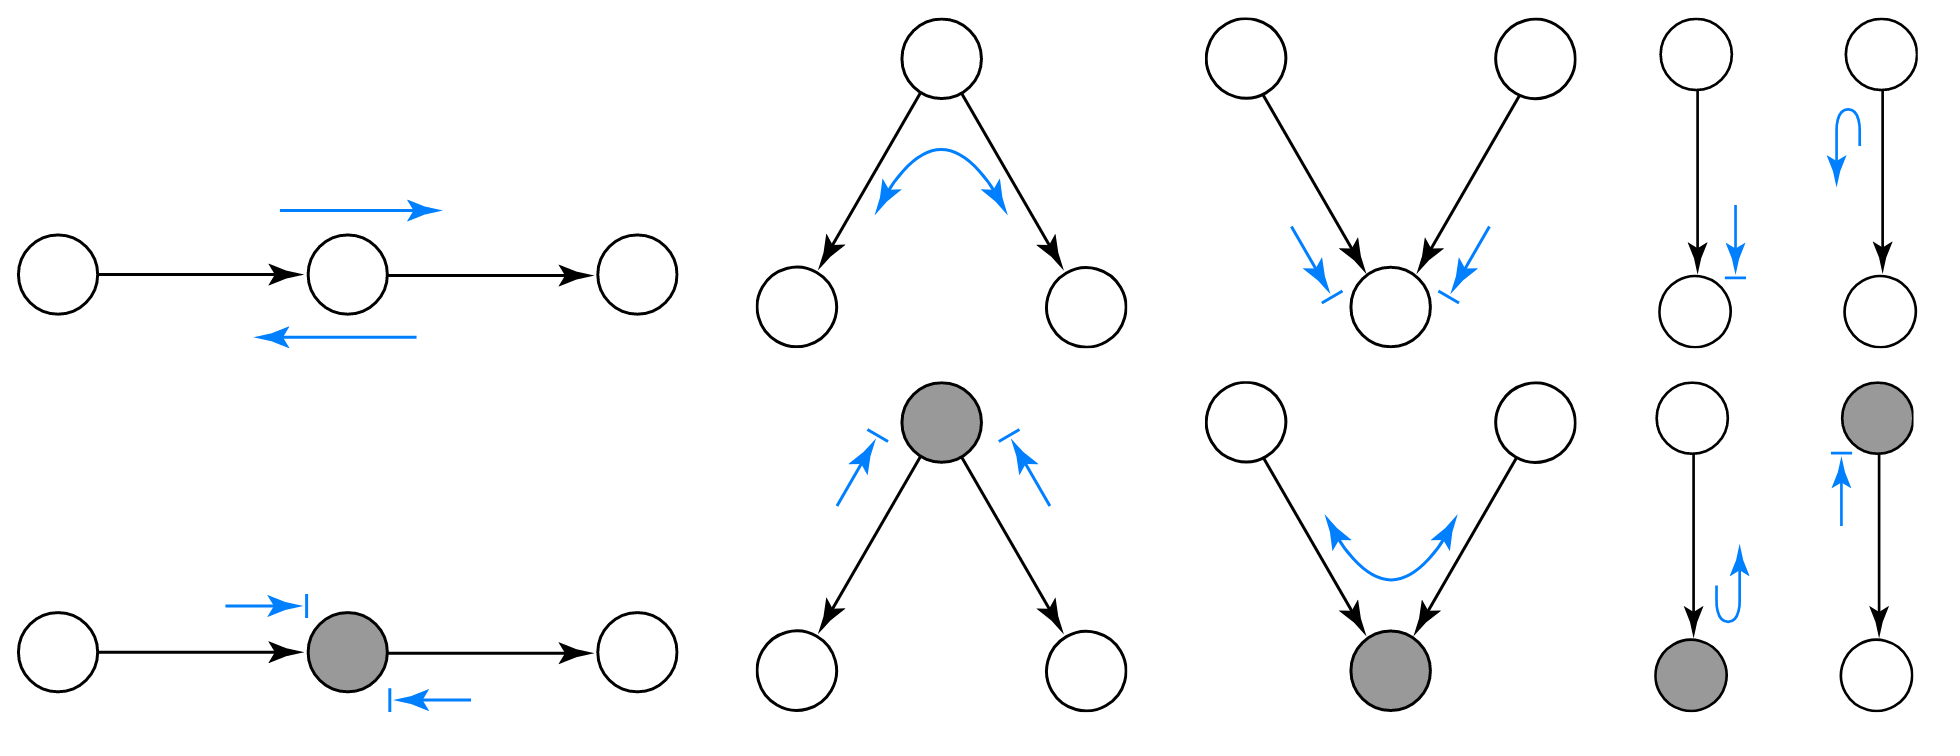
\includegraphics[width=0.7\linewidth]{img/img3.png}
        \caption{Additive Treatment Effect}
        \label{fig:1-sub1}
    \end{subfigure}%
    \begin{subfigure}{.5\textwidth}
        \centering
        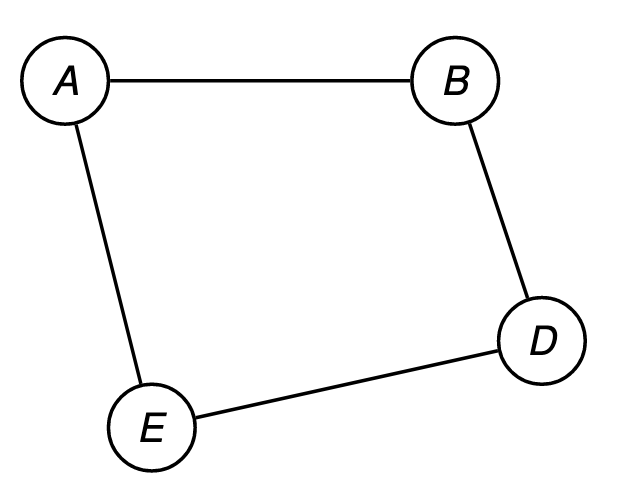
\includegraphics[width=0.7\linewidth]{img/img4.png}
        \caption{Multiplicative Treatment Effect}
        \label{fig:1-sub2}
    \end{subfigure}
    \end{figure}
\end{remark}

\begin{definition}{\textbf{(Kernel Probability Density Estimate)}}
    Let $w(x)$ be a non-negative, symmetric weight function, centered at zero and integrating to $1$. It can be standard normal density, with the following rescaled version:
    \begin{equation*}
        w_h(x) = \frac{1}{h}w\bracka{\frac{x}{h}}
    \end{equation*}
    is a rescaled version of $w$, as it approaches zero, $w_h$ becomes more concentrated and peaked around zero. On the other hand, as $h$ approaches infinity, $w_h$ becomes flat. If $X_1,\dots,X_n$ is a sample from a probability density function $p$, its esitmate is:
    \begin{equation*}
        f_h(x) = \frac{1}{n}\sum^n_{i=1}w_h(x - X_i)
    \end{equation*}
    The parameter $h$ represents bandwidth of estimating function as it controls the smoothness.
\end{definition}

\subsection{Meansure of Location}

\begin{definition}{\textbf{(Arithmetic Mean)}}
    The commonly used measure of location is the arithmetic mean, which is:
    \begin{equation*}
        \bar{x} = \frac{1}{n}\sum^n_{i=1}
    \end{equation*}
\end{definition}

\begin{remark}{\textbf{(Problem with Arithmeic Mean)}}
    By changing a single number, the arithmetic mean of a batch of numbers can be made arbitary large or smaller. Thus, when used blindly, without careful attention, the mean can produce a misleading results. Or, we need to have the measure of location that are robut or insensitive to outlier. 
\end{remark}

\begin{remark}{\textbf{(Why Sample Mean is Bad)}}
    The sample mean minimizers the log-likelihood of:
    \begin{equation*}
        \sum^n_{i=1}\bracka{\frac{(X_i - \mu)^2}{\sigma}}
    \end{equation*}
    This is the simpliest case of least square estimate. The outlier have a great effect on this estimate, as the deviation of $\mu$ from $X_i$ is measured by square of their difference.
\end{remark}

\begin{definition}{\textbf{(Median)}}
    It is a middle value of the ordered observation; if the sample size is even, the median is the average of the $2$ middle values. 
\end{definition}

\begin{proposition}{\textbf{(Confidence Interval)}}
    We can show that, given the population median $\eta$ and the interval between the order statistics $(X_{(k)}, X_{(n-k+1)})$
    \begin{equation*}
        P(X_{(k)} \le \eta \le X_{(n-k+1)}) = 1 - \frac{1}{2^{n-1}}\sum^{k-1}_{j=0}
    \end{equation*}
\end{proposition}
\begin{proof}
    The coverage probability of this interval is:
    \begin{equation*}
    \begin{aligned}
        P(X_{(k)} \le \eta \le X_{(n-k+1)}) &= 1 - P(\eta < X_{(k)} \text{ or } \eta > X_{n-k+1}) \\
        &= 1 - P(\eta < X_{(k)}) - P(\eta > X_{(n-k+1)})
    \end{aligned}
    \end{equation*}
    Since the event are mutually exclusive. To evaluate both terms, we note that:
    \begin{equation*}
    \begin{aligned}
        &P(\eta > X_{(n-k+1)}) = \sum^{k-1}_{j=0} \mathbb{P}(j \text{ observations} > \eta) \\
        &P(\eta < X_{(k)}) = \sum^{k-1}_{j=0} \mathbb{P}(j \text{ observations } < \eta)
    \end{aligned}
    \end{equation*}
    The median satisfies $P(X_i > \eta ) = P(X_i < \eta) = 1/2$, since $n$ observations $X_1,\dots,X_n$ are independent and identically distributed, the distribution of the number of observation greater than median is binomial with $n$ trials and probability $1/2$:
    \begin{equation*}
        P(j \text{ observations } > \eta) = \frac{1}{2}\begin{pmatrix}
            n \\ j
        \end{pmatrix}
    \end{equation*}
    and, so we have:
    \begin{equation*}
        P(\eta > X_{(n-k+1)}) = \frac{1}{2^n}\sum^{k-1}_{j=0}\begin{pmatrix}
            n \\ j
        \end{pmatrix}
    \end{equation*}
    This is the same for $P(\eta < X_{(k)})$ due to symmetry. Plugging it back to finish the proof
\end{proof}

\begin{remark}
    Median can be seen as the minimizer of the following loss:
    \begin{equation*}
        \sum^n_{i=1}\abs{\frac{X_i - \mu}{\sigma}}
    \end{equation*}
    Here, large deviation are not weighted as heavily, making median robust. The proof follows from the fact that the dervative of absolute is $\operatorname{sgn}(\cdot)$, and so the loss is zero when the positive $x - \mu$ (of the normalized data ) is equal to the negative item $x - \mu$, which is where the median situates. 
\end{remark}

\begin{definition}{\textbf{(Trimmed Mean)}}
    The $100\alpha\%$ trimmed mean consider the valuse that is between the lower $100\alpha\%$ and the higher $100\alpha\%$, as we can write it as:
    \begin{equation*}
        \bar{x}_\alpha = \frac{x_{[n\alpha] + 1} + \cdots + x_{(n - [n\alpha])}}{n - 2[n\alpha]}
    \end{equation*}
    where $[n\alpha]$ denotes the greatest integer less than or equal to $n\alpha$.
\end{definition}

\begin{definition}{\textbf{(M-Estimates)}}
    Consider the class of esitmates called $M$-estimates, where it is a minimizer:
    \begin{equation*}
        \sum^n_{i=1}\Psi\bracka{\frac{X_i - \nu}{\sigma}}
    \end{equation*}
    where $\Psi$ is the weight function that is a compromise between weight function for mean and median. 
\end{definition}

\begin{remark}{\textbf{(Measure of Dispersion)}}
    The most commonly used measure is sample standard deviation, where it is given as:
    \begin{equation*}
        S^2 = \frac{1}{n-1}\sum^n_{i=1}(X_i - \bar{X})^2
    \end{equation*}
    Using $n-1$ as divisor gives unbiased estimate. But like a sample mean standard deviation is sensitive to outlying observation. Two simple robust measures alternative are:
    \begin{itemize}
        \item Interquartile range (IQR): Differences between $2$ sample quantiles.
        \item Median absolute deviation from the median (MAD): If data are $x_1,\dots,x_n$ with median $\tilde{x}$, then MAD is the median of number $\abs{x_1,\dots,x_n}$. 
    \end{itemize}
\end{remark}



\section{Belief Propagation: Interpretation}

\subsection{Introduction}

\begin{definition}{\textbf{(Loopy Propagation)}}
    The joint distribution for \emph{any} graph is given by:
    \begin{equation*}
        P(\mathcal{X}) = \frac{1}{Z}\prod_{\text{nodes } i} f_i(\boldsymbol x_i) \prod_{\text{edges } (ij)} f_{ij}(\boldsymbol x_i, \boldsymbol x_j)
    \end{equation*}
    Message computed recusively with few guarantee of convergence as we have the following message:
    \begin{equation*}
        M_{j\rightarrow i} = \sum_{\boldsymbol x_j} f_{ij}(\boldsymbol x_i, \boldsymbol x_j)f_j(\boldsymbol x_j)\prod_{l \in \operatorname{ne}(j)\backslash\brackc{i}} M_{l\rightarrow j}(\boldsymbol x_j)
    \end{equation*}
    The marginal distribution are approximation in general:
    \begin{equation*}
    \begin{aligned}
        &P(\boldsymbol x_i) \approx b_i(\boldsymbol x_i) \propto f_i(\boldsymbol x_i)\prod_{k\in\operatorname{ne}(i)}M_{k\rightarrow i}(\boldsymbol x_i) \\
        &P(\boldsymbol x_i, \boldsymbol x_j) \approx b_{ij}(\boldsymbol x_i, \boldsymbol x_j) \propto f_{ij}(\boldsymbol x_i, \boldsymbol x_j)f_i(\boldsymbol x_i)f_j(\boldsymbol x_j)\prod_{k\in\operatorname{ne}(i)\backslash \brackc{j}} M_{k\rightarrow i}(\boldsymbol x_i)\prod_{l\in\operatorname{ne}(j)\backslash \brackc{i}}M_{l\rightarrow j}(\boldsymbol x_j)
    \end{aligned}
    \end{equation*}
\end{definition}

\begin{remark}{\textbf{(Dealing with Loops)}}
    There are various way to deal with loop as we have:
    \begin{itemize}
        \item The belief propagation posterior marginal are approximate on all non-tree because over-counted, but converged approximate are frequently found to be good. 
        \item Converge can be seen in: Tree, Graph with single step, Distribution with weak iteraction, Graph with long (and weak) loops, and Gaussian network (variance may also converged).
        \item Damping, as it is a common approach to encorate of EP:
        \begin{equation*}
            M^\text{new}_{i\rightarrow j}(\boldsymbol x_j) = (1-\alpha)M^\text{old}_{i\rightarrow j} + \alpha\sum_{\boldsymbol x_i}f_{ij}(\boldsymbol x_i, \boldsymbol x_j)f_i(\boldsymbol x_i) \prod_{k\in\operatorname{ne}(i)\backslash\brackc{j}}M_{k\rightarrow i}(\boldsymbol x_i)
        \end{equation*}
        \item Variable can be groupped into cliques to improve accuracy: region graph approximate, cluster variable method, and junction graph.
    \end{itemize} 
\end{remark}

\subsection{Message Based EP}

\begin{proposition}{\textbf{(Loopy BP as Message-Based EP)}}
    One can consider the connection between message-based EP and loopy BP, as they are equivalent.
\end{proposition}
\begin{proof}
    Consider the appoximate pairwise factor $\tilde{f}_{ij}$ as product of messages:
    \begin{equation*}
        f_{ij}(\boldsymbol x_i, \boldsymbol x_j) \approx \tilde{f}_{ij}(\boldsymbol x_i, \boldsymbol x_j) = M_{i\rightarrow j}(\boldsymbol x_j)M_{j\rightarrow i}(\boldsymbol x_i)
    \end{equation*}
    Consider the approximation of the factorized distribution:
    \begin{equation*}
    \begin{aligned}
        P(\mathcal{X}) &\approx \frac{1}{Z}\prod_{\text{nodes}(i)}f_i(\boldsymbol x_i) \prod_{\text{edges}(ij)}\tilde{f}_{ij}(\boldsymbol x_i, \boldsymbol x_j) \\
        &= \frac{1}{Z}\prod_{\text{nodes}(i)}\bracka{f_i(\boldsymbol x_i)\prod_{j\in\mathcal{N}(i)}M_{j\rightarrow i}(\boldsymbol x_i)} = \prod_{\text{nodes}(i)}b_i(\boldsymbol x_i)
    \end{aligned}
    \end{equation*}
    with multiple factors for $\boldsymbol x_i$, which we consider the update on EP to be:
    \begin{itemize}
        \item \emph{Deletion}: Consider the following $P(\mathcal{X})$ as we have:
        \begin{equation*}
        \begin{aligned}
            P_{\neg ij}&(X_i, X_j) = \sum_{c \ne i, j} \frac{P(\mathcal{X})}{\tilde{f}(X_i, X_j)} = \sum_{c \ne i, j} \frac{P(\mathcal{X})}{ M_{i\rightarrow j}(\boldsymbol x_j) M_{j\rightarrow i}(\boldsymbol x_i)} \\ 
            &= \frac{1}{\tilde{f}(X_i, X_j)}\sum_{c \ne i, j}f_i(\boldsymbol x_i)f_j(\boldsymbol x_j)\prod_{k\in\mathcal{N}(i)}M_{k\rightarrow i}(\boldsymbol x_i)\prod_{l\in\mathcal{N}(j)}M_{l\rightarrow j}(\boldsymbol x_j) \bracka{\prod_{s\ne i, j} f_s(\boldsymbol x_s) \prod_{t\in\mathcal{N}(s)}  M_{t\rightarrow s} (\boldsymbol x_s) } \\
            &= f_i(\boldsymbol x_i)f_j(\boldsymbol x_j)\prod_{k\in\mathcal{N}(i) \backslash j}M_{k\rightarrow i}(\boldsymbol x_i)\prod_{l\in\mathcal{N}(j)\backslash i}M_{l\rightarrow j}(\boldsymbol x_j)\sum_{c \ne i, j}\bracka{\prod_{s\ne i, j} f_s(\boldsymbol x_s) \prod_{t\in\mathcal{N}(s)}  M_{t\rightarrow s} (\boldsymbol x_s) } \\
            &= f_i(\boldsymbol x_i)f_j(\boldsymbol x_j)\prod_{k\in\mathcal{N}(i) \backslash j}M_{k\rightarrow i}(\boldsymbol x_i)\prod_{l\in\mathcal{N}(j)\backslash i}M_{l\rightarrow j}(\boldsymbol x_j) \\
        \end{aligned}
        \end{equation*}
        \item \emph{Projection}: We consider minimizing the KL-divergence as we have:
        \begin{equation*}
            \brackc{M^\text{new}_{i\rightarrow j}, M^\text{new}_{j\rightarrow i}} = \argmin{M_{i\rightarrow j}, M_{j\rightarrow i}} \operatorname{KL}\brackb{ f_{ij}(\boldsymbol x_i, \boldsymbol x_j) q_{\neg ij}(\boldsymbol x_i, \boldsymbol x_j) \Big\| M_{j\rightarrow i}(\boldsymbol x_i) M_{i\rightarrow j}(\boldsymbol x_j)q_{\neg ij}(\boldsymbol x_i, \boldsymbol x_j) }
        \end{equation*}
        To solve this KL-divergence, this is obvious, as $q_{\neg ij}(\cdot)$ can be factorized and so the minimizer is the marginal between $f_{ij}(\cdot)q_{\neg ij}(\cdot)$, which means that:
        \begin{equation*}
        \begin{aligned}
            M_{i\rightarrow j}^\text{new}(\boldsymbol x_j)q_{\neg ij}(\boldsymbol x_i, \boldsymbol x_j)& = \sum_{\boldsymbol x_j}\bracka{f_{ij}(\boldsymbol x_i, \boldsymbol x_j) f_j(\boldsymbol x_j)\prod_{l\in\mathcal{N}(j)\backslash i}M_{l\rightarrow j}(\boldsymbol x_j) } \underbrace{f_i(\boldsymbol x_i)\prod_{k\in\mathcal{N}(i) \backslash j}M_{k\rightarrow i}(\boldsymbol x_i)}_{q_{\neg ij}(\boldsymbol x_i)} \\
            \implies& M_{i\rightarrow j}^\text{new}(\boldsymbol x_j) = \sum_{\boldsymbol x_j}\bracka{f_{ij}(\boldsymbol x_i, \boldsymbol x_j) f_j(\boldsymbol x_j)\prod_{l\in\mathcal{N}(j)\backslash i}M_{l\rightarrow j}(\boldsymbol x_j) }
        \end{aligned}
        \end{equation*}
        This is the Loopy BP update, and so both of the are equivalent. 
    \end{itemize}
\end{proof}

\begin{remark}{\textbf{(Comments on the Loopy BP and EP)}}
    There are some observation that we can make in the equivalent between loopy BP and EP algorithm:
    \begin{itemize}
        \item Unlike EP, this message based EP doesn't need $2$ separate approximate as we have in the normal EP.
        \item This message based EP is loopy graph can be seen as a more constraint on approximate site and not just exponential family factor but the product of exponential family message. 
        \item On a tree, message forward EP finds the same marginal as standard EP as the messages are calculated the same way. Similarly, the pairwise marginal can be found after converge by compute $\tilde{P}(z_{i - 1}, z_i)$
        \item Factorization still remain valid even when original site lies in the appoximation exponential family already, so the loopy BP can be seen as form of EP. 
        \item This doesn't help us with understanding the convergence property of EP.
    \end{itemize}
\end{remark}

\subsection{Reparameterized on Tree}

\begin{remark}{\textbf{(Tree-Based Representation)}}
    We consider the joint factorization, which can be represented:
    \begin{equation*}
    \begin{aligned}
        P(\mathcal{X}) &= \frac{1}{Z}\prod_{\operatorname{nodes}(i)} f_i(\boldsymbol x_i)\prod_{\operatorname{edges}(ij)} f_{ij}(\boldsymbol x_i, \boldsymbol x_j) \qquad \text{(Undirected Tree)} \\
        &= P(\boldsymbol x_i)\prod_{i\ne r}P(\boldsymbol x_i | \boldsymbol x_{\text{pa}(i)}) \qquad \text{(Directed Rooted Tree)} \\
        &= \prod_{\operatorname{nodes}(i)}P(\boldsymbol x_i)\prod_{\operatorname{edges}(ij)}\frac{P(\boldsymbol x_i, \boldsymbol x_j)}{P(\boldsymbol x_i)P(\boldsymbol x_j)}  \qquad \text{(Pairwise Marginal)} \\
    \end{aligned}
    \end{equation*}
    The last on requires that $\sum_{\boldsymbol x_j}P(\boldsymbol x_i, \boldsymbol x_j) = P(\boldsymbol x_i)$. 
    \begin{itemize}
        \item The unidrected tree isn't unique as if we multiply the factor $f_{ij}(\boldsymbol x_i, \boldsymbol x_j)$ by $g(\boldsymbol x_i)$ and dividing $f_i(\boldsymbol x_i)$ by the same $g(\boldsymbol x_i)$ doesn't change the distribution. 
        \item BP can be seen as iteractive replacement of $f_i(\boldsymbol x_i)$ by local marginal of $p_{ij}(\boldsymbol x_i, \boldsymbol x_j)$ along with corresponding representation of $f_{ij}(\boldsymbol x_i, \boldsymbol x_j)$ (recall the Hugin propagation)
        \item Converged BP on a tree finds $P(\boldsymbol x_i)$ and $P(\boldsymbol x_i, \boldsymbol x_j)$ allowing up to transform the undirected tree to pairwise marginal. 
    \end{itemize}
\end{remark}

\begin{remark}{\textbf{(Reparameterization in Tree)}}
    To consider the tree based reparameterization, we want to transform the representation from undirected tree to pairwise marginal as:
    \begin{equation*}
        \prod_{\operatorname{nodes}(i)} f_i(\boldsymbol x_i)\prod_{\operatorname{edges}(ij)} f_{ij}(\boldsymbol x_i, \boldsymbol x_j) \implies \prod_{\operatorname{nodes}(i)}P(\boldsymbol x_i)\prod_{\operatorname{edges}(ij)}\frac{P(\boldsymbol x_i, \boldsymbol x_j)}{P(\boldsymbol x_i)P(\boldsymbol x_j)}
    \end{equation*}
    We will define the $f^0_{ij} = f_{ij}$, while the singleton factor to be $f^0_1 = p^0_1 = 1$, we consider the following update: The update is based on the fact that we will act on the factors \emph{as if} it is actually representing the probabilities: We will consider such a procedure on a node that has $2$ incoming messages. 
    \begin{itemize}
        \item Starting with joint, where if we multiply it by adjacent factors we get $P(\boldsymbol x_i, \boldsymbol x_j)$ i.e
        \begin{equation*}
            p^{(n)}(\boldsymbol x_i, \boldsymbol x_j) = \frac{1}{Z_{ij}^{(n)}} f^{(n-1)}_i(\boldsymbol x_i)f^{(n-1)}_{ij}(\boldsymbol x_i, \boldsymbol x_j) f^{(n-1)}_j(\boldsymbol x_j)
        \end{equation*}
        \item Finding the marginal, as we have:
        \begin{equation*}
            f^{(n)}_i(\boldsymbol x_i) = p^{(n)}(\boldsymbol x_i) = \sum_{\boldsymbol x_j}p^{(n)}(\boldsymbol x_i, \boldsymbol x_j) = f^{(n-1)}_i(\boldsymbol x_i)\underbrace{\sum_{\boldsymbol x_j} f^{(n-1)}_{ij}(\boldsymbol x_i, \boldsymbol x_j) f^{(n-1)}_j(\boldsymbol x_j)}_{M_{j\rightarrow i}}
        \end{equation*}
        \item To keep the normalization correctly, we divide the message so that the update on one passing giving us normalized term:
        \begin{equation*}
            f^{(n)}_{ij} = \frac{f^{(n-1)}_{ij}(\boldsymbol x_i, \boldsymbol x_j)}{M_{j\rightarrow i}(\boldsymbol x_j)}
        \end{equation*}
        \item We now consider the next step with the next incoming message from node $k$ to node $i$:
        \begin{equation*}
        \begin{aligned}
            p^{(n)}(\boldsymbol x_i, \boldsymbol x_k) &= \frac{1}{Z_{ik}^{(n)}} f^{(n)}_i(\boldsymbol x_i)f^{(n-1)}_{ik}(\boldsymbol x_i, \boldsymbol x_j) f^{(n-1)}_k(\boldsymbol x_j) \\
            &= \frac{1}{Z_{ik}^{(n)}} f^{(n-1)}_i(\boldsymbol x_i)M_{j\rightarrow i}(\boldsymbol x_i) f^{(n-1)}_{ik}(\boldsymbol x_i, \boldsymbol x_k) f^{(n-1)}_k(\boldsymbol x_k) \\
        \end{aligned}
        \end{equation*}
        \item Finding the singleton factor by marginalization
        \begin{equation*}
            f^{(n)}_i(\boldsymbol x_i) = f^{(n-1)}_i(\boldsymbol x_i)M_{j\rightarrow i}(\boldsymbol x_i) \underbrace{\sum_{\boldsymbol x_k}f^{(n-1)}_{ik}(\boldsymbol x_i, \boldsymbol x_k) f^{(n-1)}_k(\boldsymbol x_k)}_{M_{k\rightarrow i}}
        \end{equation*}
        \item And so, the normalization correction on the joint factor is:
        \begin{equation*}
            f^{(n)}_{ik} = \frac{f^{(n-1)}_{ik}(\boldsymbol x_i, \boldsymbol x_k)}{ M_{k\rightarrow i}(\boldsymbol x_i) }
        \end{equation*}
    \end{itemize}
    We perform this update throughout the tree, which we do it in forward (e.g $i\rightarrow j$) and backward (e.g $j\rightarrow i$) manner, which gives us:
    \begin{equation*}
    \begin{aligned}
        &f^{(\infty)}_i(\boldsymbol x_i) = \prod_{j\operatorname{ne}(i)}M_{j\rightarrow i}(\boldsymbol x_i) = P(\boldsymbol x_i) \\
        &\begin{aligned}[t]
            f^{(\infty)}_{ij}(\boldsymbol x_i, \boldsymbol x_j) &= \frac{f_{ij}(\boldsymbol x_i, \boldsymbol x_j)}{M_{j\rightarrow i}(\boldsymbol x_i)M_{i\rightarrow j}(\boldsymbol x_j)} \\
            &= \frac{\prod_{k \in \operatorname{ne}(i)\backslash j}M_{k\rightarrow i}f_{ij}(\boldsymbol x_i, \boldsymbol x_j)\prod_{l \in \operatorname{ne}(j)\backslash i}M_{l\rightarrow i}(\boldsymbol x_j)}{\prod_{k \in \operatorname{ne}(i)\backslash j}M_{k\rightarrow i} M_{j\rightarrow i}(\boldsymbol x_i)M_{i\rightarrow j}(\boldsymbol x_j) \prod_{l \in \operatorname{ne}(j)\backslash i}M_{l\rightarrow i}(\boldsymbol x_j) } \\
            &= \frac{\prod_{k \in \operatorname{ne}(i)\backslash j}M_{k\rightarrow i}f_{ij}(\boldsymbol x_i, \boldsymbol x_j)\prod_{l \in \operatorname{ne}(j)\backslash i}M_{l\rightarrow i}(\boldsymbol x_j)}{\prod_{k \in \operatorname{ne}(i)}M_{k\rightarrow i} \prod_{l \in \operatorname{ne}(j)}M_{l\rightarrow i}(\boldsymbol x_j) } \\
            &= \frac{P(\boldsymbol x_i, \boldsymbol x_j)}{P(\boldsymbol x_i)P(\boldsymbol x_j)}
        \end{aligned}
    \end{aligned}
    \end{equation*}
    the equation follows from the result from belief propagation.This kind of reparameterization allows us to avoid double counting, which is essentially a book-keeping method, espescially the normalizing part (there will be a case where the factor cancel with unnecessary message from singleton factor, as intended). 
\end{remark}

\begin{remark}{\textbf{(Comments on the BP on non-tree)}}
    If this converges in a non-tree setting, then we have locally consistent belief i.e:
    \begin{equation*}
        p(\mathcal{X}) \propto \prod_i b(\boldsymbol x_i) \prod_{ij}\frac{b(\boldsymbol x_i, \boldsymbol x_j)}{b(\boldsymbol x_i)b(\boldsymbol x_j)} \quad \text{ such that } \quad \sum_{\boldsymbol x_j}b(\boldsymbol x_i, \boldsymbol x_j) = b(\boldsymbol x_i)
    \end{equation*}
    But it doesn't need to be globally consistent:
    \begin{equation*}
        \sum_{\mathcal{X}_{\neg i}}\bracka{\prod_i b(\boldsymbol x_i) \prod_{ij}\frac{b(\boldsymbol x_i, \boldsymbol x_j)}{b(\boldsymbol x_i)b(\boldsymbol x_j)}} \ne b(\boldsymbol x_i)
    \end{equation*}
    This kind of marginal is called \emph{pseudo-marginal}. 
\end{remark}

\begin{remark}{\textbf{(Message Schedule Scheme)}}
    We consider update the belief on each \emph{subtree} of the graph and passing message on each subtree, looping through all the subtree until converge:
    \begin{figure}[H]
        \centering
        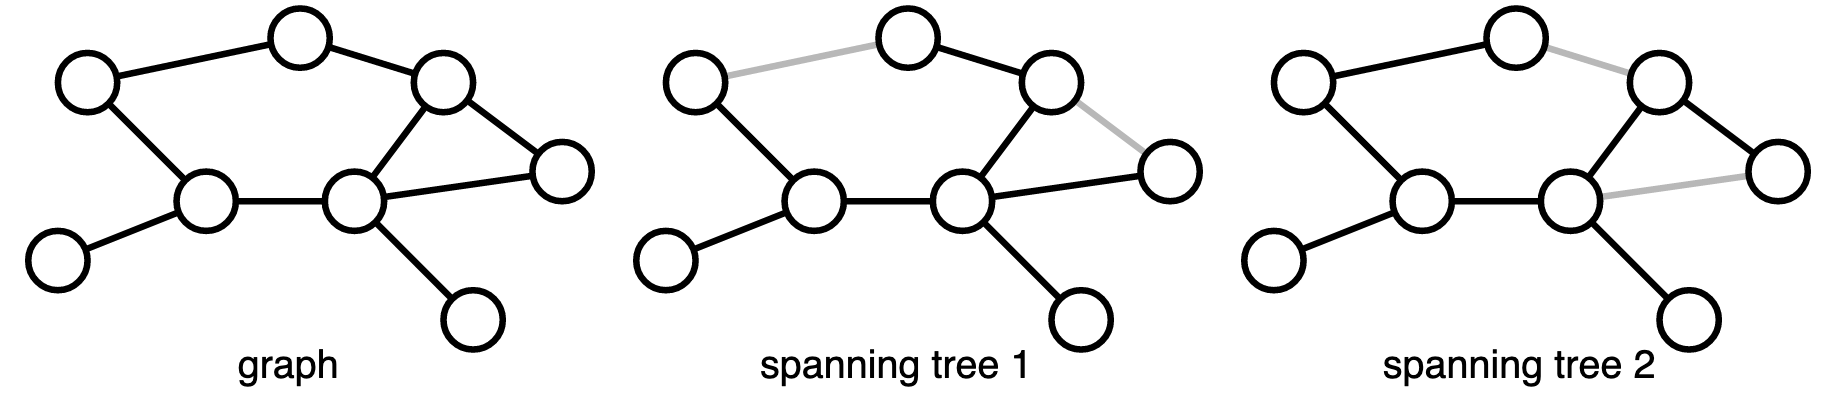
\includegraphics[width=10cm]{img/img16.png}
    \end{figure}  
    And, we now that the following updates steps:
    \begin{equation*}
    \begin{aligned}
        P(\mathcal{X}) 
        &= \frac{1}{Z}\prod_{\operatorname{nodes}(i)} f^{(0)}_i(\boldsymbol x_i)\prod_{\operatorname{edges}(ij)} f^{(0)}_{ij}(\boldsymbol x_i, \boldsymbol x_j) \\
        &= \frac{1}{Z}\prod_{\operatorname{nodes}(i) \in T_1} f^{(0)}_i(\boldsymbol x_i)\prod_{\operatorname{edges}(ij) \in T_1} f^{(0)}_{ij}(\boldsymbol x_i, \boldsymbol x_j)\bracka{\prod_{\operatorname{edges}(ij) \not\in T_1} f^{(0)}_{ij}(\boldsymbol x_i, \boldsymbol x_j)} \\
        &\text{(Update)} \\
        &= \frac{1}{Z}\prod_{\operatorname{nodes}(i) \in T_1} f^{(1)}_i(\boldsymbol x_i)\prod_{\operatorname{edges}(ij) \in T_1} f^{(1)}_{ij}(\boldsymbol x_i, \boldsymbol x_j)\bracka{\prod_{\operatorname{edges}(ij) \not\in T_1} f^{(1)}_{ij}(\boldsymbol x_i, \boldsymbol x_j)} \\
        &\text{(Next Tree)} \\
        &= \frac{1}{Z}\prod_{\operatorname{nodes}(i) \in T_2} f^{(1)}_i(\boldsymbol x_i)\prod_{\operatorname{edges}(ij) \in T_2} f^{(1)}_{ij}(\boldsymbol x_i, \boldsymbol x_j)\bracka{\prod_{\operatorname{edges}(ij) \not\in T_2} f^{(1)}_{ij}(\boldsymbol x_i, \boldsymbol x_j)} \\
        &\cdots
    \end{aligned}
    \end{equation*}
    where we have, when we got a new tree, 
    \begin{equation*}
        f^{(1)}_i(\boldsymbol x_i) = P^{T_1}(\boldsymbol x_i)\qquad f^{(1)}_{ij}(\boldsymbol x_i, \boldsymbol x_j) = \frac{P^{T_1}(\boldsymbol x_i, \boldsymbol x_j)}{P^{T_1}(\boldsymbol x_i)P^{T_2}(\boldsymbol x_j)} 
    \end{equation*}
    If the process converges, suppose it converge to:
    \begin{equation*}
        P(\mathcal{X}) = \frac{1}{Z}\prod_{\operatorname{nodes}(i)} f_i^{(\infty)}(\boldsymbol x_i)\prod_{\operatorname{edges}(ij)} f_{ij}^{(\infty)}(\boldsymbol x_i, \boldsymbol x_j)
    \end{equation*}
    where for any tree $T$ in the graph, we have:
    \begin{equation*}
        f_i^{(\infty)} = P^T(\boldsymbol x_i)\qquad f_{ij}^{(\infty)} = \frac{P^T(\boldsymbol x_i, \boldsymbol x_j)}{P^T(\boldsymbol x_i)P^T(\boldsymbol x_j)}
    \end{equation*}
    This means that the local marginal of all subtree are consistent with each other, and the pseudo-marginal is valid belief of any of the subtree, as this is stronger constriant. 
\end{remark}

\subsection{Bathe Free Energy}

\begin{remark}{\textbf{(Introduction to Bathe Free Energy)}}
    In reparameterization view, BP solves for marginal belief $b_{ij}(\boldsymbol x_i, \boldsymbol x_j)$ and $b_i(\boldsymbol x_i) = \sum_{\boldsymbol x_j}b_{ij}(\boldsymbol x_i, \boldsymbol x_j)$  such that:
    \begin{equation*}
        P(\mathcal{X}) \propto \prod_if_i(\boldsymbol x_i)\prod_{ij}f_{ij}(\boldsymbol x_i, \boldsymbol x_j) \propto \prod_ib_i(\boldsymbol x_i)\prod_{ij}\frac{b_{ij}(\boldsymbol x_i, \boldsymbol x_j)}{b_i(\boldsymbol x_i)b_j(\boldsymbol x_j)}
    \end{equation*}
    Loopy BP is a set of fixed point equation for finding stationary of an objective function called Bathe free energy, which is defined in terms of locally consistent belief (pseudo-marginal) $b_i\ge0$ and $b_{ij}\ge0$ such that:
    \begin{equation*}
        \sum_{\boldsymbol x_i} b_i(\boldsymbol x_i) = 1 \qquad \sum_{\boldsymbol x_j}b_{ij}(\boldsymbol x_i, \boldsymbol x_j) = b_i(\boldsymbol x_i)
    \end{equation*}
\end{remark}

\begin{definition}{\textbf{(Bathe Free Energy)}}
    We define it in the form of:
    \begin{equation*}
        \mathcal{F}_\text{bathe}(b) = \mathcal{E}_\text{bathe}(b) + \mathcal{H}_\text{bathe}(b) 
    \end{equation*}
    Both terms are approximated so that it corresponds to variational likelihood terms:
    \begin{itemize}
        \item Bathe average energy is the expected log-joint evaluate as though the pseudomarginal were correct:
        \begin{equation*}
            \mathcal{E}_\text{bathe}(b) = \sum_i\sum_{\boldsymbol x_i} b_i(\boldsymbol x_i)\log f_i(\boldsymbol x_i) + \sum_{ij}\sum_{\boldsymbol x_i\boldsymbol x_j} b_{ij}(\boldsymbol x_i, \boldsymbol x_j)\log f_{ij}(\boldsymbol x_i, \boldsymbol x_j)
        \end{equation*}
        \item Bathe entropy is the sum of pseudomarginal entropies corrected for pairwise (pseudo-)interaction, but neglecting higher-order dependence:
        \begin{equation*}
        \begin{aligned}
            \mathcal{H}_\text{bathe}(b) &= \sum_i H[b_i] - \sum_{ij}\operatorname{KL}[b_{ij} | b_ib_j] \\
            &= -\sum_i\sum_{\boldsymbol x_i} b_i(\boldsymbol x_i)\log b_i(\boldsymbol x_i) - \sum_{ij}\sum_{\boldsymbol x_i\boldsymbol x_j}b_{ij}(\boldsymbol x_i, \boldsymbol x_j)\log \frac{b_{ij}(\boldsymbol x_i, \boldsymbol x_j)}{b_i(\boldsymbol x_i)b_j(\boldsymbol x_j)}
        \end{aligned}
        \end{equation*}
    \end{itemize}
    On tree, both belief and the bathe entropy expression are correct i.e $\mathcal{F}_\text{bathe} = \mathcal{F}$. The update rule can be recoved from finding the fixed point. 
\end{definition}

\begin{proposition}{\textbf{(Fixed Point for Bathe Free Energy)}}
    The fixed point for Bathe free energy is:
    \begin{equation*}
    \begin{aligned}
        &b_i(\boldsymbol x_i) \propto f_i(\boldsymbol x_i)\prod_{j\in\operatorname{ne}(i)}\exp(-\xi_{ij}(\boldsymbol x_i)) \\
        &b_{ij}(\boldsymbol x_i, \boldsymbol x_j) \propto f_{ij}(\boldsymbol x_i, \boldsymbol x_j)b_i(\boldsymbol x_i)b_j(\boldsymbol x_j)\exp(\xi_{ij}(\boldsymbol x_i) + \xi_{ij}(\boldsymbol x_j)) \\
        &\exp(-\xi_{ij}(\boldsymbol x_i)) \propto \sum_{\boldsymbol x_j}f_{ij}(\boldsymbol x_i, \boldsymbol x_j)f_j(\boldsymbol x_j)\prod_{l\in\operatorname{ne}(j)\backslash i}\exp(-\xi_{ij}(\boldsymbol x_j)) \\
    \end{aligned}
    \end{equation*}
\end{proposition}
\begin{proof}
    We find the Lagragian with local consistency and normalization, which is given as:
    \begin{equation*}
    \begin{aligned}
        \mathcal{L} = \sum_{i}&\sum_{\boldsymbol x_i}b_i(\boldsymbol x_i)\log f_i(\boldsymbol x_i) + \sum_{ij}\sum_{\boldsymbol x_i\boldsymbol x_j}b_{ij}(\boldsymbol x_i, \boldsymbol x_j)\log f_{ij}(\boldsymbol x_i,\boldsymbol x_j) \\
        &- \sum_i\sum_{\boldsymbol x_i}b_i(\boldsymbol x_i)\log b_i(\boldsymbol x_i)-\sum_{ij}\sum_{\boldsymbol x_i\boldsymbol x_j}b_{ij}(\boldsymbol x_i, \boldsymbol x_j)\log\frac{b_{ij}(\boldsymbol x_i, \boldsymbol x_j)}{b_i(\boldsymbol x_i)b_j(\boldsymbol x_j)} \\
        &+ \sum_i\xi_i\bracka{\sum_{\boldsymbol x_i}b_i(\boldsymbol x_i)-1} \\
        &+ \sum_{ij}\brackb{ \sum_{\boldsymbol x_i}\xi_{ij}(\boldsymbol x_{i})\bracka{\sum_{\boldsymbol x_j}b_{ij}(\boldsymbol x_i, \boldsymbol x_j) - b_i(\boldsymbol x_i)} + \sum_{\boldsymbol x_j}\xi_{ij}(\boldsymbol x_j)\bracka{ \sum_{\boldsymbol x_i}b_{ij}(\boldsymbol x_i, \boldsymbol x_j) - b_j(\boldsymbol x_j) } }
    \end{aligned}
    \end{equation*}
    Setting the derivate to zero, which gives us the solution:
    \allowdisplaybreaks
    \begin{align*}
        &\begin{aligned}[t]
            \frac{\partial}{\partial b_i(\boldsymbol x_i)} &= \log f_i(\boldsymbol x_i) - \log b_i(\boldsymbol x_i) + \sum_{j\in\operatorname{ne}(j)}\sum_{\boldsymbol x_j}\frac{b_{ij}(\boldsymbol x_i, \boldsymbol x_j)}{b_i(\boldsymbol x_i)} + \xi_i - \sum_{j\in\operatorname{ne}(i)}\xi_{ij}(\boldsymbol x_i) + \const = 0 \\
            &\implies b_i(\boldsymbol x_i) \propto f_i(\boldsymbol x_i)\prod_{j\in\operatorname{ne}(i)} \exp(-\xi_{ij}(\boldsymbol x_i))
        \end{aligned} \\
        &\begin{aligned}[t]
            \frac{\partial f}{\partial b_{ij}(\boldsymbol x_i, \boldsymbol x_j)} &= \log f_{ij}(\boldsymbol x_i, \boldsymbol x_j) - \log b_{ij}(\boldsymbol x_i, \boldsymbol x_j) + \log b_i(\boldsymbol x_i)b_j(\boldsymbol x_j) + \xi_{ij}(\boldsymbol x_i) + \xi_{ji}(\boldsymbol x_j) + \const = 0 \\
            &\implies b_{ij}(\boldsymbol x_i, \boldsymbol x_j) \propto f_{ij}(\boldsymbol x_i, \boldsymbol x_j) b_i(\boldsymbol x_i)b_j(\boldsymbol x_j) \exp(\xi_{ij}(\boldsymbol x_i) + \xi_{ji}(\boldsymbol x_j))
        \end{aligned}
    \end{align*}
    To solve for $\xi_{ij}(\boldsymbol x_i)$ by enforcing the constant $\sum_{\boldsymbol x_j}b_{ij}(\boldsymbol x_i, \boldsymbol x_j) = b_i(\boldsymbol x_i)$ where we have:
    \begin{equation*}
    \begin{aligned}
        &\sum_{\boldsymbol x_j} b_{ij}(\boldsymbol x_i, \boldsymbol x_j) \propto \sum_{\boldsymbol x_j}f_{ij}(\boldsymbol x_i, \boldsymbol x_j)b_i(\boldsymbol x_i)b_j(\boldsymbol x_j)\exp(\xi_{ij}(\boldsymbol x_i) + \xi_{ji}(\boldsymbol x_j)) \\
        \implies& b_i(\boldsymbol x_i) \propto b_i(\boldsymbol x_i)\exp(\xi_{ij}(\boldsymbol x_i))\sum_{\boldsymbol x_j}f_{ij}(\boldsymbol x_i, \boldsymbol x_j)b_j(\boldsymbol x_j)\exp(\xi_{ji}(\boldsymbol x_j)) \\
        \implies& \begin{aligned}[t]
            \exp(-\xi_{ij}(\boldsymbol x_i)) &\propto \sum_{\boldsymbol x_j}f_{ij}(\boldsymbol x_i, \boldsymbol x_j)b_j(\boldsymbol x_j)\exp(\xi_{ji}(\boldsymbol x_j)) \\
            &= \sum_{\boldsymbol x_j}f_{ij}(\boldsymbol x_i, \boldsymbol x_j)f_j(\boldsymbol x_j)\prod_{l\in\operatorname{ne}(j)\backslash i}\exp(-\xi_{ji}(\boldsymbol x_j))
        \end{aligned}
    \end{aligned}
    \end{equation*}
\end{proof}

\begin{remark}{\textbf{(Interpretation of Results)}}
    Comparing with BP, we have the message to be of the form of $M_{j\rightarrow i}(\boldsymbol x_i) = \exp(-\xi_{ij}(\boldsymbol x_i))$. The fixed point for bathe free energy recovers the message passing rule:
    \begin{itemize}
        \item Stable Fixed point of loopy BP are stationary point of Bathe and local minimum of Bathe free energy. 
        \item For binary attractive netwrok: the Bathe free energy at fixed point of loopy BP provides an upperbound on the log partition function $\log P(\boldsymbol Z)$. 
        \item It is useful for learning undirected graphical model as it leads to lower bound on the log-likelihood. 
        \item Belief $b_i$ and $b_{ij}$ in loopy BP are only locally consistent pseudomarginal, not necessary consistent with marginal or the implied joint distribution. 
        \item Bathe free enerfy accounts for interaction between difference states, while variational free energy that assume independence. 
        \item The log series Plefka expansion of the log-partition $Z$: the variational energy form the first order while Bathe free energy contains higher term. 
        \item Loopy BP tends to significantly more accurate whenever it converges. 
    \end{itemize}
\end{remark}

\begin{remark}{\textbf{(Extensions and Variations)}}
    \begin{itemize}
        \item Generalized BP is a group variable together to threat their interaction exacely. 
        \item The algorithm can be derived so that the Bathe free energy at every step and thus guarantee the convergence. Similarly, convex alternative and we will converge to unique global maximum. 
        \item The treatment of loopy Viterbi or max-product algorithm is difference. 
    \end{itemize}
\end{remark}

\section{Online Learning 2: Bandits}

\begin{definition}{\textbf{(Partial Feedback Protocal)}}
    We cosnider the following setting:
    \begin{algorithm}[H]
        \caption{Partial Feedback Control}
        \begin{algorithmic}[1]
            \For {$i=1,2,\cdots, T$}
                \State Predict $\hat{y}_t \in [n]$
                \State Observe loss of prediction $l_{t, \hat{y}_t}\in[0, 1]$
            \EndFor
        \end{algorithmic} 
    \end{algorithm}
    We have the following goal:
    \begin{equation*}
        \sum^m_{t=1}l_{t, \hat{y_t}} - \min_{i\in[n]}\sum^m_{t=1}l_{t, i} \le o(m)
    \end{equation*}
    This is the same as the regret. Please note that we didn't get to see all loss function that is induced by the prediction.
\end{definition}

\begin{definition}{\textbf{(Unbiased Estimation)}}
    An estimator $\hat{\theta}$  estimate a parameter $\theta$ of a distribution from a sample is unbiased if we can show that $\mathbb{E}[\hat{\theta}] = \theta$.
\end{definition}

\begin{example}
    Suppose $X_1,\dots,X_n$ are iid random variable for a distribution with mean $\mu$, then:
    \begin{equation*}
        \hat{\theta} = \frac{1}{n}(X_1+\dots+X_n)
    \end{equation*}
    is an unbiased estimate of $\mu$
\end{example}

\begin{example}
    Suppose $X$ is a random variable with the discrete unifrom distribution over $\brackc{1,\dots,n}$. Suppose $n$ is unknown and we wish to estimate it. 
    \begin{itemize}
        \item The estimate $\hat{\theta}_1 = X$ is the maximum likelihood estimator, since $\mathcal{L}(\theta, X = x) = 1/\theta$ is maximized when $\theta = x$. Then we have:
        \begin{equation*}
            \mathbb{E}[\hat{\theta}_1 ; \theta = n] = \sum^n_{x=1}\frac{x}{n} = \frac{n+1}{2}
        \end{equation*}
        \item And so, $\hat{\theta}_2 = 2x - 1$ is unbiased estimator, which is:
        \begin{equation*}
            \mathbb{E}[\hat{\theta}_2 ; \theta = n] = \sum^n_{x=1}\frac{1}{n}(2x - 1) = 2\sum^n_{x=1} \frac{1}{n} (2x - 1) = 2\sum^n_{x=1}\frac{1}{n}x -\sum^n_{x=1}\frac{1}{n} = n
        \end{equation*}
    \end{itemize}
\end{example}

\begin{remark}{\textbf{(Assumption and Estimation)}}
    Suppose, we have a distribution $D_i$ over $[0, 1]$ for each $i\in[n]$ arms. For each arm $i$, we use iid sample $l_{t, i}$ for $D_i$. Suppose, we play $i$ on trials $S_{t, i}\subseteq[t]$, then:
    \begin{equation*}
        \hat{\mu}_{t, i} = \sum_{t\in S_i} \frac{l_{t, i}}{|S_i|}
    \end{equation*}
    This is unbiased estimator of $\mu_i$. Now, we can consider the usage as we have:
    \begin{itemize}
        \item We can use a concentration inequality that allows us to quantitatively estimate the likelihood to estimate differently for the parameter. 
        \item Using the observation, the algorithm UCB balances exploration and exploitation to obtain good regret bounds for this method. 
        \item Suppose tha tthe underlying $D_i$ is changing over time (being $D_{t, i}$):
        \begin{equation*}
            \mu_{t, i} = \frac{\sum^t_{j=1} \mathbb{E}[l_{j,t}]}{t}
        \end{equation*}
        where $S_i = [t]$. However, if we only have $S_{t, i} = [t]$, then we have no information about the other arms. 
        \item We need to have simultaneous unbiased estimate for all arms $S$
    \end{itemize}
\end{remark}

\begin{definition}{\textbf{(Importance Weighting)}}
    We have the following series of observation:
    \begin{itemize}
        \item Suppose $X$ is a random variable over $\mathbb{R}$ with a mean $\mu$. By definition, $\mathbb{E}[X] = \mu$ and $\hat{\theta}_1 = X$ is an unbiased estimator of the mean. 
        \item Consider the biased coin $Z_p$ with outcome $1$ with probability $p$. Suppse, we have the estimator $\hat{\theta}_0$ setting to equal to $X/p$ if $Z_p = 1$. 
        \item Its expectation is equal to:
        \begin{equation*}
            \mathbb{E}[\hat{\theta}_0] = \mathbb{P}(Z_p = 1)(X/p) + 0 \mathbb{P}(Z_p = 0) = (p)(X/p) + (1-p)(0) = X
        \end{equation*}
        This is unbiased. 
    \end{itemize} 
\end{definition}

\begin{definition}{\textbf{(Hallucinated Loss Vector)}}
    We generalize this to obtain an unbiased estimator of $l_t$ in the bandit setting. Given $\boldsymbol v_t \in \Delta_n$  by the relation tha t$\hat{y}_t \sim \boldsymbol v_t$. The unbiased estimator $l^n_t$ or $\boldsymbol k_t$ with respected to $\boldsymbol v_t$ is given as:
    \begin{equation*}
        \bracka{l^h_{t, i} = \frac{l_{t, i}}{v_{t, i}} \mathbb{I}[i = \hat{y}_t] }_{i \in [n]}
    \end{equation*}
\end{definition}

\begin{remark}{\textbf{(Expectation of Hallucinated Loss Vector)}}
    Observed that $l^h_t$ is unbiased for all $i\in[n]$ since we have:
    \begin{equation*}
        \mathbb{E}_{\hat{y}_t, \boldsymbol v_t}[l^h_{t, i}] = \sum^n_{j=1}v_{t, j}\frac{l_{t, i}}{v_{t, i}} \mathbb{I}[i = j] = l_{t, i}
    \end{equation*}
    We have unbiased estimator for all arms by only observing the single arm. We can apply the hedge to $l^h_t$ requires bounded loss vector. We can use more careful analysis of the hedge. 
    % \begin{itemize}
    %     \item We will be given an expected regret bound and there will be some subtleties in the source of randomness. 
    %     \item This will be clarify the adversariable model that generates the loss $\boldsymbol l_1,\dots,\boldsymbol l_m$
    % \end{itemize}
\end{remark}

\begin{definition}{\textbf{(EXP3)}}    
    Exponential-Weight algorithm for Exploration and Exploitation is given by:
    \begin{algorithm}[H]
        \caption{EXP3}
        \begin{algorithmic}[1]
            \State \textbf{Initialize}: $\eta \in (0, \infty)$
            \State Set $\boldsymbol v_1 = (1/n, \dots, 1/n)$
            \For {$i=1,2,\cdots, T$}
                \State Sample $\hat{y}_t \sim \boldsymbol v_t$
                \State Observe Loss $l_{t, \hat{y}} \in [0, 1]$
                \State Construct Hallucinated Loss vector:
                \begin{equation*}
                    l^h_t = \bracka{l^h_{t, i} = \frac{l_{t, i}}{v_{t, i}} \mathbb{I}[i = \hat{y}_t] }_{i \in [n]}
                \end{equation*}
                \State Perform the update, for $i\in[n]$ and $Z_t = \sum^n_{i=1}v_{t,i}\exp(-\eta l^h_{t, i})$:
                \begin{equation*}
                    v_{t+1, i} = v_i\exp(-\eta l^h_{t, i})/Z_t
                \end{equation*}
            \EndFor
        \end{algorithmic} 
    \end{algorithm}
\end{definition}

\begin{lemma}  
    For any sequence of loss vector $\boldsymbol l_1,\dots,\boldsymbol l_m \in [0, 1]^n$, we have the following loss bound:
    \begin{equation*}
        \sum^m_{t=1}\boldsymbol v_t^T\boldsymbol l^h_t - \sum^m_{t=1}\boldsymbol u^T\boldsymbol l^h_t \le \frac{\ln n}{\eta} + \frac{\eta}{2}\sum^m_{t=1}\sum^n_{i=1}v_{t, i}(l^h_{t, i})^2
    \end{equation*}
    For all $\boldsymbol u \in \Delta_n$
\end{lemma}
\begin{proof}
    The lemma follows from the fact that EXP3 is just Hedge with $\boldsymbol l_t$ weighted to be $\boldsymbol l^h_t$ and the Hedge inequality is proven before. 
\end{proof}

\begin{remark}
    We can show the property of EXP3, where we consider that: we need to perform and so we may replace hallucination losses $\boldsymbol l^h_t$ with time loss $\boldsymbol l$:
    \begin{itemize}
        \item We can model some of the randomness as we use the adversarial loss $\boldsymbol l_1,\dots,\boldsymbol l_m$. 
        \item We have to bound the term $\sum^m_{t=1}\sum^n_{i=1}v_{t,i}(l^h_{t,i})^2$ and tune $\eta$
    \end{itemize}
\end{remark}

\begin{definition}{\textbf{(Deterministic Adversarial Model)}}
    We will to set $\boldsymbol l_1,\dots,\boldsymbol l_m$ before running the algorithm. The adversary is assumed to be complete given the prior knowledge, and:
    \begin{itemize}
        \item The limitation of near omniscient adversary is that it is non-adaptive. 
        \item It many simulate the stochastic model by repeatedly sample the $\mathcal{D}_1,\dots,\mathcal{D}_m$ in advance.
    \end{itemize} 
\end{definition}

\begin{theorem}
    For any sequence of loss vector $S = l_1,\dots,l_m \in [0, 1]^n$, the regret for EXP3 with $\eta = \sqrt{2\ln n/mn}$ is:
    \begin{equation*}
        \mathbb{E}[L_A(S)] - \min_i L_i \le \sqrt{2mn\ln n}
    \end{equation*}
    where $L_A(S) = \sum^m_{t=1}l_{t, \hat{y}_y}$ and $L_i = \sum^m_{t=1}l_{t, i}$
\end{theorem}
\begin{proof}
    Observe that the only source of randomness are the sample $\hat{y}_t \sim \boldsymbol v_t$. As previously argue, note that $\mathbb{E}[l^h_{t, i}] = l_{t, i}$, and we have:
    \begin{equation*}
        \mathbb{E}[\boldsymbol v_t^T\boldsymbol l^h_t] = \sum^n_{i=1}\mathbb{E}[v_{t, i}l^h_{t, i}] = \sum^n_{i=1}v_{t, i}\mathbb{E}[l^h_{t, i}] = \sum^n_{i=1}v_{t, i}l_{t, i} = \mathbb{E}[l_{t, \hat{y}_t}]
    \end{equation*}
    Similarly, we have:
    \begin{equation*}
        \mathbb{E}[(l^h_{t, i})^2] = \sum^n_{j=1}v_{t, j}\bracka{\frac{l_{t, i}}{v_{t, i}}}^2 \mathbb{I}[i = j]^2 = v_{t,i}\bracka{\frac{l_{t,i}}{v_{t, i}}}^2 = \frac{l^2_{t, i}}{v_{t, i}}
    \end{equation*}
    This implies that:
    \begin{equation*}
        \mathbb{E}\brackb{\sum^n_{i=1} v_{t, i}(l^h_{t, i})^2 } = \sum^n_{i=1}v_{t, i}\frac{l^2_{t, i}}{v_{t, i}} = \sum^n_{i=1}l^2_{t, i} \le n
    \end{equation*}
    Taking the expectation over the Hedge terms, and we have for $\boldsymbol u \in \Delta_n$:
    \begin{equation*}
        \mathbb{E}\brackb{\sum^m_{t=1}\boldsymbol v_t^T\boldsymbol l^h_t - \sum^m_{t=1}\boldsymbol u^T\boldsymbol l^h_t} \le \mathbb{E}\brackb{\frac{\ln n}{\eta} + \frac{\eta}{2}\sum^m_{t=1}\sum^n_{i=1}v_{t, i}(l^h_{t, i})^2}
    \end{equation*}
    And, so we have using the fact that: $\mathbb{E}[l^h_{t, i}] = l_{t, i}$, and the previous result with $\boldsymbol u$ being a coordinate vector, we have:
    \begin{equation*}
        \mathbb{E}\brackb{\sum^m_{t=1}\boldsymbol v_t^T\boldsymbol l^h_t} - \min_i\mathbb{E}\brackb{\sum^m_{t=1}\boldsymbol l^h_{t, i}} \le \frac{\ln n}{\eta} + \frac{\eta}{2}\mathbb{E}\brackb{\sum^m_{t=1}\sum^n_{i=1}v_{t, i}(l^h_{t, i})^2}
    \end{equation*}
    And, so we have:
    \begin{equation*}
        \mathbb{E}[L_A(S)] - \min_i L_i(S) \le \ln\frac{n}{\eta} + \frac{\eta}{2}mn
    \end{equation*}
    Substuite the $\eta = \sqrt{2\ln n/mn}$ to prove this theorem.
\end{proof}

\section{The Analysis of Categorical Data}

\subsection{Fisher's Exact Test}

\begin{remark}{\textbf{(Setting for the Tests)}}
    Let's consider the data that we are given as:
    \begin{table}[!h]
    \centering
    \begin{tabular}{lcccc}
        \toprule
        \textbf{}     & \textbf{Variation 1} & \textbf{Variation 2} & Total  \\
        \midrule
        \textbf{Category 1} & $N_{11}$ & $N_{12}$ & $n_{1.}$ \\
        \textbf{Category 2} & $N_{21}$ & $N_{22}$ & $n_{2.}$ \\
        Total & $n_{.1}$ & $n_{.2}$ & $n_{..}$ \\
        \bottomrule
    \end{tabular}
    \end{table}
    We want the see whether the count in each category is affected by the some variation of data or not (the null hypothesis is that thet are all randomly assigned). There are auxillary variables denoted (total). 
\end{remark}

\begin{remark}{\textbf{(Probability Under Null Hypothesis)}}
    Under the null hypothesis (randomly generated), and so the probability that $N_{11} = n_{11}$ is given as:
    \begin{equation*}
        p(n_{11}) = \cfrac{\begin{pmatrix}
            n_{1.} \\ n_{11}
        \end{pmatrix}\begin{pmatrix}
            n_{2.} \\ n_{21}
        \end{pmatrix}}{\begin{pmatrix}
            n_{..} \\ n_{.1}
        \end{pmatrix}}
    \end{equation*}
    We can use $N_{11}$ as the test statistics for testing the null hypothesis. We can generate the table to create $2$ sided rejects for extreme value of $N_{11}$
\end{remark}

\subsection{$\chi^2$-Test for Homogeneity}

\begin{remark}{\textbf{(Settings for $\boldsymbol \chi^2$-Test)}}
    We consider the larger setting compared to Fisher's exact test, where we comparing $J$ multinomial distribution each having $I$ categories. If the probability of $i$-th category of $j$-th multinomial is denoted as $\pi_{ij}$, the null hypothesis is:
    \begin{equation*}
        H_0 : \pi_{i1} = \pi_{i2} = \cdots = \pi_{iJ} \qquad i = 1,\dots,J
    \end{equation*}
    Under $H_0$ each of the $J$ multinomial has the same probability for the $i$-th category as $\pi_i$. 
\end{remark}

\begin{proposition}
    Under $H_0$, the MLE of the parameter $\pi_1,\pi_2,\dots,\pi_I$ are given as:
    \begin{equation*}
        \hat{\pi}_i = \frac{n_{i.}}{n_{..}} \qquad i = 1,\dots,I
    \end{equation*}
    where $n_{i.}$ is the total number of response in the $i$-th category and $n_{..}$ is the grand total number of response. 
\end{proposition}
\begin{proof}
    Since the multinomial distribution are independent:
    \begin{equation*}
    \begin{aligned}
        \operatorname{lik}(\pi_1,\pi_2,\dots,\pi_I) &= 
        \prod^J_{j=1}\begin{pmatrix}
            n_{.j} \\ n_{1j}n_{2j}\cdots n_{Ij}
        \end{pmatrix} 
        \pi^{n_{1j}}_1\pi^{n_{2j}}_2\cdots\pi^{n_{Ij}}_I \\
        &=  \pi^{n_{1j}}_1\pi^{n_{2j}}_2\cdots\pi^{n_{Ij}}_I
        \prod^J_{j=1}
        \begin{pmatrix}
            n_{.j} \\ n_{1j}n_{2j}\cdots n_{Ij}
        \end{pmatrix} 
    \end{aligned}
    \end{equation*}
    Consider maximizing the log-likelihood subject to constraint $\sum^I_{i=1}\pi_i = 1$. Introducing multiplier, we have to maximizing:
    \begin{equation*}
        \mathcal{L}(\pi, \lambda) = \sum^J_{j=1}\log  
        \begin{pmatrix}
            n_{.j} \\ n_{1j}n_{2j}\cdots n_{Ij}
        \end{pmatrix} + \sum^I_{i=1}n_{i.}\log\pi_i + \lambda\bracka{\sum^I_{i=1}\pi_i-1}
    \end{equation*}
    Now, we have:
    \begin{equation*}
    \begin{aligned}
        &\frac{\partial l}{\partial \pi_i} = \frac{n_{i.}}{\pi_i} + \lambda \qquad i =1,\dots,I \\
        \iff&\hat{\pi}_i = -\frac{n_i}{\lambda}
    \end{aligned}
    \end{equation*}
    Summing over both sides and applying the constraint, we find that $\lambda = -n_{..}$ and the theorem is proven.
\end{proof}

\begin{definition}{\textbf{(Peason's $\boldsymbol \chi^2$-Test)}}
    For $j$-th multinomial, the expected count in the $i$-th category is the etimated probability of the cell times the total number of observation for $j$-th multinomial:
    \begin{equation*}
        E_{ij} = \frac{n_{i.}}{n_{..}} n_{.j}
    \end{equation*}
    This gives us the Peason's $\chi^2$-statistics as we have:
    \begin{equation*}
        X^2 = \sum^I_{i=1}\sum^J_{j=1} \frac{(O_{ij} - E_{ij})^2}{E_{ij}} =  \sum^I_{i=1}\sum^J_{j=1} \frac{(n_{ij} - n_{i.}n_{.j}/n_{..})^2}{n_{i.}n_{.j}/n_{..}}
    \end{equation*}
    For large sample size, the approximate null distribution of this statistics is $\chi^2$. We have the degree of freedom are number of independent counts minus the number of independent parameter:
    \begin{itemize}
        \item Each multinomial has $I-1$ independent counts, since the total are fixed. 
        \item $I-1$ independent parameter have been estimated.
    \end{itemize}
    And so the degree of freedom are given as $J(I-1)-(I-1) = (I-1)(J-1)$. 
\end{definition}

\subsection{$\chi^2$-Test of Independent}

\begin{definition}{\textbf{(Contingency Table)}}
    We will discuss the statistical analysis of sample of size $n$ cross-classifed in table with $I$ rows and $J$ columns. This configuration is called contingency table.
\end{definition}

\begin{remark}{\textbf{(Settings for the Test)}}
    We are interested in the relationship between factors on the table. The joint distribution of the counts $n_{ij}$ where $i=1,\dots,I$ and $j=1,\dots,J$ is multinomial with cell probabilities denoted as:
    \begin{equation*}
        \pi_{i.} = \sum^J_{j=1}\pi_{ij} \qquad
        \pi_{.j} = \sum^I_{i=1}\pi_{ij} \qquad
    \end{equation*}
    Both are the marginal probability that the observation will fall in $i$-th row or $j$-columns. If both row and columns are independent of each other then: $\pi_{ij} = \pi_{i.}\pi_{.j}$. This leads to the following null hypothesis:
    \begin{equation*}
        H_0 : \pi_{ij} = \pi_{i.}\pi_{.j} \qquad i = 1,\dots,I \quad j = 1,\dots,J
    \end{equation*}
\end{remark}

\begin{remark}{\textbf{(Defining the $\chi^2$-Test)}}
    Let's consider the MLE estimate under each hypothesis 
    \begin{itemize}
        \item Under $H_0$ is the MLE of $\pi_{ij}$ is given as:
        \begin{equation*}
            \hat{\pi}_{ij} = \hat{\pi}_{i.}\hat{\pi}_{.j} = \frac{n_{i.}}{n}\frac{n_{.j}}{n}
        \end{equation*}
        \item Under alternative MLE of $\pi_{ij}$ is given as:
        \begin{equation*}
            \tilde{\pi}_{ij} = \frac{n_{ij}}{n}
        \end{equation*}
    \end{itemize}
    Now we consider $\chi^2$-test as we have:
    \begin{equation*}
        X^2 = \sum^I_{i=1}\sum^J_{j=1} \frac{(O_{ij} - E_{ij})^2}{E_{ij}} = \sum^I_{i=1}\sum^J_{j=1} \frac{(n_{ij} -  (n_{i.}n_{.j})/n)^2}{ (n_{i.}n_{.j})/n}
    \end{equation*}
    where $O_{ij}$ are the observation count as we have $n_{ij}$. The expected count is $E_{ij} = n\hat{\pi}_{ij} = (n_{i.}n_{.j})/n$. 
    \begin{itemize}
        \item Let's consider the degree of freedom as under $\Omega$, the cell probabilities sum to $1$ as it has the dimension to be $IJ-1$. 
        \item Under the null hypothesis, the marginal probabilities are estimated from the data are specified to $(I-1)+(J-1)$
    \end{itemize}
    We have the following degree of freedom: 
    \begin{equation*}
        \operatorname{df} = IJ - 1 - (I-1) - (J-1) = (I-1)(J-1)
    \end{equation*}
\end{remark}

\subsection{Matched-Pairs Designs}

\begin{remark}{\textbf{(Setting for the test)}}
    We consider the following table 
    \begin{table}[H]
    \centering
    \begin{tabular}{lcccc}
        \toprule
        \textbf{}     & \textbf{No Cure (Sibling)} & \textbf{Cure (Sibling)} & Total  \\
        \midrule
        \textbf{No Cure (Patient)} & $\pi_{11}$ & $\pi_{12}$ & $\pi_{1.}$ \\
        \textbf{Cure (Patient)} & $\pi_{21}$ & $\pi_{22}$ & $\pi_{2.}$ \\
        Total & $\pi_{.1}$ & $\pi_{.2}$ & $1$ \\
        \bottomrule
    \end{tabular}
    \end{table}
    The appropriate null hypothesis is $\pi_{i.} = \pi_{.i}$, where $i = 1,2$ (the probabilities of cure and no cure should be the same for patient and sibling), and so we have:
    \begin{equation*}
        \pi_{11} + \pi_{12} = \pi_{11} + \pi_{21} \qquad 
        \pi_{12} + \pi_{22} = \pi_{21} + \pi_{22} \qquad 
    \end{equation*}
    The equation is simplified to $\pi_{12} = \pi_{21}$, where the null hypothesis is thus:
    \begin{equation*}
        H_0 : \pi_{12} = \pi_{21}
    \end{equation*}
\end{remark}

\begin{proposition}{\textbf{(MLE of Cell Probabilities)}} 
    Under the $H_0$, the MLE of the cell probabilities are:
    \begin{equation*}
        \hat{\pi}_{11} = \frac{n_{11}}{n} \qquad  \hat{\pi}_{22} = \frac{n_{22}}{n} \qquad \hat{\pi}_{12} = \hat{\pi}_{21} = \frac{n_{12} + n_{21}}{2n}
    \end{equation*}
\end{proposition}

\begin{definition}{\textbf{(McNemar's Test)}}
    The contribution to the $\chi^2$ statistics from $n_{11}$ and $n_{22}$ cells are equal to zero. The remainder of statistics is:
    \begin{equation*}
        X^2 =\frac{[n_{12} - (n_{12} + n_{21})/2]^2}{(n_{12} + n_{21})/2} + \frac{[n_{21} - (n_{12} + n_{21})/2]^2}{(n_{12} + n_{21})/2} = \frac{(n_{12} - n_{21})^2}{n_{12} + n_{21}}
    \end{equation*}
    Let's consider the degree of freedom, as under $\Omega$ there are $3$ free parameters (since there are $4$ probability that are constrianted to one). On the null hypothesis, there are addiitonal constraint $\pi_{12} = \pi_{21}$ so there are $2$ free parameter. Thus we have $1$ degree of freedom.
\end{definition}

\subsection{Odd Ratios}

\begin{definition}{\textbf{(Odd)}}
    If an event $A$ has probability $P(A)$ of occuring, the odds of $A$ occuring are defined as (please note that this works with conditional probability):
    \begin{equation*}
        \operatorname{odds}(A) = \frac{P(A)}{1-P(A)} \implies P(A) = \frac{\operatorname{odds}(A)}{1+\operatorname{odds}(A)}
    \end{equation*}
\end{definition}

\begin{definition}{\textbf{(Odds Ratio)}}
    We have the following:
    \begin{equation*}
        \Delta = \frac{\operatorname{odds}(D | X)}{\operatorname{odds}(D|\bar{X})}
    \end{equation*}
    where $\bar{X}$ is the complementary element. This measures the influenced of some event $X$ to the event $D$.
\end{definition}

\begin{remark}{\textbf{(Setting for Test)}}
    We consider how the odds and odds ratio could be estimated by sampling from a population with joint and marignal probability defined as:
    \begin{table}[H]
    \centering
    \begin{tabular}{lcccc}
        \toprule
        \textbf{}     & $\bar{D}$ & $D$ & Total  \\
        \midrule
        $\bar{X}$ & $\pi_{00}$ & $\pi_{01}$ & $\pi_{0.}$ \\
        $X$ & $\pi_{10}$ & $\pi_{11}$ & $\pi_{1.}$ \\
        Total & $\pi_{.0}$ & $\pi_{.1}$ & $1$ \\
        \bottomrule
    \end{tabular}
    \end{table}
    With this notation, as we have:
    \begin{equation*}
        P(D | X) =\frac{\pi_{11}}{\pi_{10} + \pi_{11}} \qquad P(D|\bar{X}) = \frac{\pi_{01}}{\pi_{00} + \pi_{01}}
    \end{equation*}
    And, so we have:
    \begin{equation*}
        \operatorname{odds}(D | X) = \frac{\pi_{11}}{\pi_{10}}
        \qquad \operatorname{odds}(D | \bar{X}) = \frac{\pi_{01}}{\pi_{00}} \qquad \Delta = \frac{\pi_{11}\pi_{00}}{\pi_{01}\pi_{10}}
    \end{equation*}
    The product of diagonal probabilities in the preceding table divided by the product of the off-diagonal probabilities.
\end{remark}

\begin{remark}{\textbf{(Ways to Sample the Data)}}
    \begin{itemize}
        \item \emph{Naive Sample}: We can consider drawing a random sample from the entire population. But if the event $D$ is rare, the total sample size would have to be quite large to guarantee that substantial number of $D$ is included. 
        \item \emph{Prospective Study}: Fixed number of even $X$ and $\bar{X}$ are sample, then incidence of $D$ are compared. This allow use to compare $P(D|X)$ and $P(D|\bar{X})$ and the odd ratio. However $\pi_{ij}$ can not be estiamte from the data. 
        \item \emph{Retrospective Study}: We fixed number of $D$ and $\bar{D}$ and we compared the number of $X$ and $\bar{X}$. We can estimate $P(X|D)$ and $P(X|\bar{D})$ by the proportion. But, we can't estimate $P(D|X)$ and $P(D|\bar{X})$ or the joint probability.
    \end{itemize}
\end{remark}

\begin{proposition}
    The odds ratio on the contingency table $\Delta$ can be expressed as:
    \begin{equation*}
        \Delta = \frac{\operatorname{odds}(X | D)}{\operatorname{odds}(X|\bar{D})}
    \end{equation*}
\end{proposition}
\begin{proof}
    This follows from the calculation of $P(X|D)$ and $1-P(X|D)$ where we have:
    \begin{equation*}
        P(X | D) = \frac{\pi_{11}}{\pi_{01} + \pi_{11}} \qquad 1 - P(X|D) = \frac{\pi_{01}}{\pi_{01} + \pi_{11}} \qquad \operatorname{odds}(X |D) = \frac{\pi_{11}}{\pi_{01}} \qquad \operatorname{odds}(X | \bar{D}) = \frac{\pi_{10}}{\pi_{00}}
    \end{equation*}
    We can see that the odds ratio $\Delta$ can be expressed as above, thus complete the proof.
\end{proof}

\begin{remark}{\textbf{(Retrospective Study - Odds Ratio)}}
    We can't find the odds ratio of given the restrospective study but we can approximate it. Using the above result. where we replace $\pi_{ij}$ with $n_{ij}$ where $n$ is the count of the observation. 
\end{remark}

\begin{remark}{\textbf{(Statistical Testing)}}
    Since the value $\hat{\Delta}$ is non-linear function of the counts, we will have to use the boostrap to construct the approximation of the distribution $\hat{\Delta}$
\end{remark}



% \begin{algorithm}[H]
%     \caption{$PSRO_{RN}$}
% 	\begin{algorithmic}[1]
% 	    \State \textbf{Input}: Initial Population $\mathcal{B}_1$
% 		\For {$i=1,2,\cdots, T$}
% 		    \State $p \leftarrow \text{Nash}(A_{\mathcal{B}_i})$
% 		    \For {agent $v_i$ with positive mass in $p_t$}
%                 \State $v_{i+1} \leftarrow \text{oracle}(v_i, \sum_{w \in \mathcal{B}_i} p[i](\phi_{v_i}(\cdot))_+)$
%             \EndFor
%             \State $\mathcal{B}_{i+1} = \mathcal{B} \cup \{v_{i+1} : \text{as updated above}\}$
% 		\EndFor
% 	\end{algorithmic} 
% \end{algorithm}

% \begin{table}[!h]
%   \centering
%   \begin{tabular}{lc}
%     \toprule
%     \textbf{Methods/Metrics}     & \textbf{Accuracy}  \\
%     \midrule
%     Logistic Regression          & $48.26 \pm 0.0f0$ \\
%     Support Vector Machine       & $48.91 \pm 0.00$  \\
%     Random Forest Classifier     & $44.38 \pm 1.57$  \\
%     \midrule
%     Multi-Dimensional ELO        & $34.51 \pm 3.12$  \\
%     TrueSkill\texttrademark      & $44.99 \pm 0.00$  \\
%     \bottomrule
%   \end{tabular}
  
%   \caption{}
  
%   \label{table}
% \end{table}

% \begin{AutoMultiColItemize}
%   \item Item 1
%   \item Item 2
%   \item Item 3
%   \item Item 4
%   \item Item 5
%   \item Item 6
% \end{AutoMultiColItemize}


% \bibliographystyle{plain}
% \bibliography{references}
\end{document}
